\documentclass[aspectratio=169, xcolor={dvipsnames,table}]{beamer}
\usepackage[utf8]{inputenc}
\usepackage[T1]{fontenc}
\usepackage{lmodern} 
\usepackage{tikz}
\usepackage{booktabs}
\usepackage{colortbl}
\usetikzlibrary{calc, shapes.multipart, arrows.meta, shadows}

% -------------------------
% Original Modern Color Palette
% -------------------------
\definecolor{Navy}{HTML}{0F172A}      % Deep Slate Blue
\definecolor{Emerald}{HTML}{10B981}   % Vibrant Green
\definecolor{LightGray}{HTML}{F8FAFC} % Very Light Gray Background
\definecolor{DarkGray}{HTML}{334155}  % Muted text
\definecolor{Coral}{HTML}{F43F5E}     % Alert/Accent

% -------------------------
% Beamer Theme Settings
% -------------------------
\setbeamertemplate{navigation symbols}{}
\setbeamercolor{background canvas}{bg=LightGray}
\setbeamercolor{normal text}{fg=Navy}
\setbeamercolor{frametitle}{bg=Navy, fg=white}
\setbeamercolor{itemize item}{fg=Emerald}

% Custom Frame Title (Sleek Geometric Header)
\setbeamertemplate{frametitle}{
    \begin{tikzpicture}[remember picture, overlay]
        \fill[Navy] (current page.north west) rectangle ($(current page.north east) - (0, 1.2)$);
        \fill[Emerald] (current page.north west) rectangle ($(current page.north west) + (0.15, -1.2)$);
        \node[anchor=west, white, font=\Large\bfseries] at ($(current page.north west) + (0.4, -0.6)$) {\insertframetitle};
    \end{tikzpicture}
    \vspace{0.6cm}
}

% Command for Vertical Model Metric Tables
\newcommand{\slidemetrics}[5]{
    \renewcommand{\arraystretch}{1.3}
    \begin{tabular}{|p{3.5cm}|p{2cm}|}
        \hline
        \rowcolor{Navy!10} \textbf{\color{Navy}Metric} & \textbf{\color{Navy}Value} \\
        \hline
        \textbf{Model} & #1 \\
        \hline
        \textbf{MAE} & #2 \\
        \hline
        \textbf{RMSE} & #3 \\
        \hline
        \textbf{MAPE} & #4\% \\
        \hline
        \textbf{R$^2$ Score} & #5 \\
        \hline
    \end{tabular}
}

\begin{document}

% ==========================================
% SLIDE 1: HERO TITLE SLIDE
% ==========================================
\begin{frame}[plain]
\begin{tikzpicture}[remember picture, overlay]
    % Clean Background
    \fill[Navy] (current page.north west) rectangle (current page.south east);
    
    % Sharp Geometric Accents
    \fill[Emerald] (current page.south west) -- (current page.north west) -- ($(current page.north west) + (5,0)$) -- ($(current page.south west) + (8,0)$) -- cycle;
    \fill[Navy!90!black] (current page.south west) -- (current page.north west) -- ($(current page.north west) + (4.8,0)$) -- ($(current page.south west) + (7.8,0)$) -- cycle;
    
    % Text Content
    \node[anchor=west, white, font=\Huge\bfseries] at ($(current page.west) + (0.5, 1.5)$) {Applied Forecasting};
    \node[anchor=west, Emerald, font=\LARGE\bfseries] at ($(current page.west) + (0.5, 0.4)$) {Human Stress Prediction Pipeline};
    
    \node[anchor=west, white, font=\small] at ($(current page.west) + (0.5, -0.8)$) {\textbf{Dataset:} WESAD (Wearable Chest-Worn Sensors)};
    \node[anchor=west, white, font=\small] at ($(current page.west) + (0.5, -1.3)$) {\textbf{Target:} High-Resolution Continuous Stress Intensity};
    \node[anchor=west, white, font=\small] at ($(current page.west) + (0.5, -1.8)$) {\textbf{Models:} 13 Architectures (Statistical, ML, DL)};
    
    % Group Info Block
    \node[anchor=south east, align=right, white] at ($(current page.south east) + (-0.8, 0.8)$) {
        \textbf{Group Members}\\[0.1cm]
        Nilesh Mori (202301473)\\
        Harsh Maheriya (202301470)\\
        Dhanush Pillai (202301483)\\
        Megh Jagtap (202303040)\\[0.3cm]
        \textcolor{Emerald}{May 10, 2026}
    };
\end{tikzpicture}
\end{frame}

% ==========================================
% SLIDE 2: INTRODUCTION
% ==========================================
\begin{frame}{Problem Statement}
\begin{columns}[T]
    \begin{column}{0.48\textwidth}
        \textbf{The Reactive Baseline}\\[0.2cm]
        Most mental-health wearables notify users \textit{after} an anxiety or stress event has occurred. This is a classification problem (Stressed vs. Not Stressed).
        \vspace{0.4cm}
        
        \textbf{The Proactive Forecasting Challenge}\\[0.2cm]
        Can we use a user's recent physiological history (EDA, HR, TEMP) to \textbf{accurately predict future stress intensity} before it happens?
    \end{column}
    \begin{column}{0.48\textwidth}
        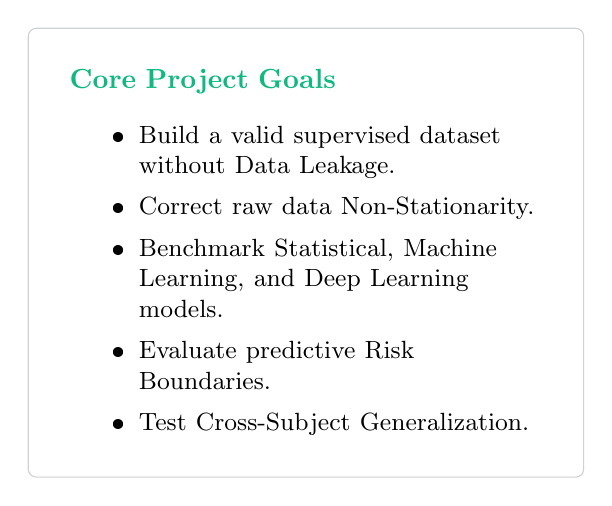
\begin{tikzpicture}
            \node[fill=white, draw=Navy!20, rounded corners=3pt, inner sep=15pt, text width=6cm] {
                \textbf{\color{Emerald}Core Project Goals}\\[0.3cm]
                \small
                \begin{itemize}
                    \item Build a valid supervised dataset without Data Leakage.
                    \item Correct raw data Non-Stationarity.
                    \item Benchmark Statistical, Machine Learning, and Deep Learning models.
                    \item Evaluate predictive Risk Boundaries.
                    \item Test Cross-Subject Generalization.
                \end{itemize}
            };
        \end{tikzpicture}
    \end{column}
\end{columns}
\end{frame}

% ==========================================
% SLIDE 3: DATASET OVERVIEW
% ==========================================
\begin{frame}{Dataset Description: WESAD}
\textbf{Wearable Stress and Affect Detection (WESAD)} provides high-frequency recordings. We extracted the chest-worn signals due to their superior clinical fidelity.
\vspace{0.4cm}

\begin{columns}
    \begin{column}{0.35\textwidth}
        \textbf{Monitored Signals:}
        \begin{itemize}
            \item \textbf{EDA:} Electrodermal Activity
            \item \textbf{TEMP:} Skin Temperature
            \item \textbf{HR:} Heart Rate
        \end{itemize}
        \vspace{0.2cm}
        \textbf{Transformation:}\\
        Raw 700Hz data was downsampled to 1Hz using mean aggregation to reduce jitter and computational load.
    \end{column}
    \begin{column}{0.6\textwidth}
        \textbf{Processed Continuous Data (First 5 Rows):}
        \begin{table}
            \small
            \begin{tabular}{ccccc}
                \toprule
                \rowcolor{Navy!10} \textbf{Second} & \textbf{HR} & \textbf{EDA} & \textbf{TEMP} & \textbf{Stress Score} \\
                \midrule
                0 & 77.77 & 5.24 & 30.12 & 0.6945 \\
                1 & 77.81 & 5.47 & 30.10 & 0.7137 \\
                2 & 80.96 & 6.27 & 30.09 & 0.7961 \\
                3 & 71.52 & 6.41 & 30.09 & 0.7654 \\
                4 & 66.85 & 6.20 & 30.09 & 0.7264 \\
                \bottomrule
            \end{tabular}
        \end{table}
    \end{column}
\end{columns}
\end{frame}

% ==========================================
% SLIDE 4: DISTRIBUTIONS
% ==========================================
\begin{frame}{Feature Distribution \& Variance Analysis}
Understanding the underlying density of physiological signals is critical before applying machine learning regressors.
\vspace{0.2cm}
\begin{center}
    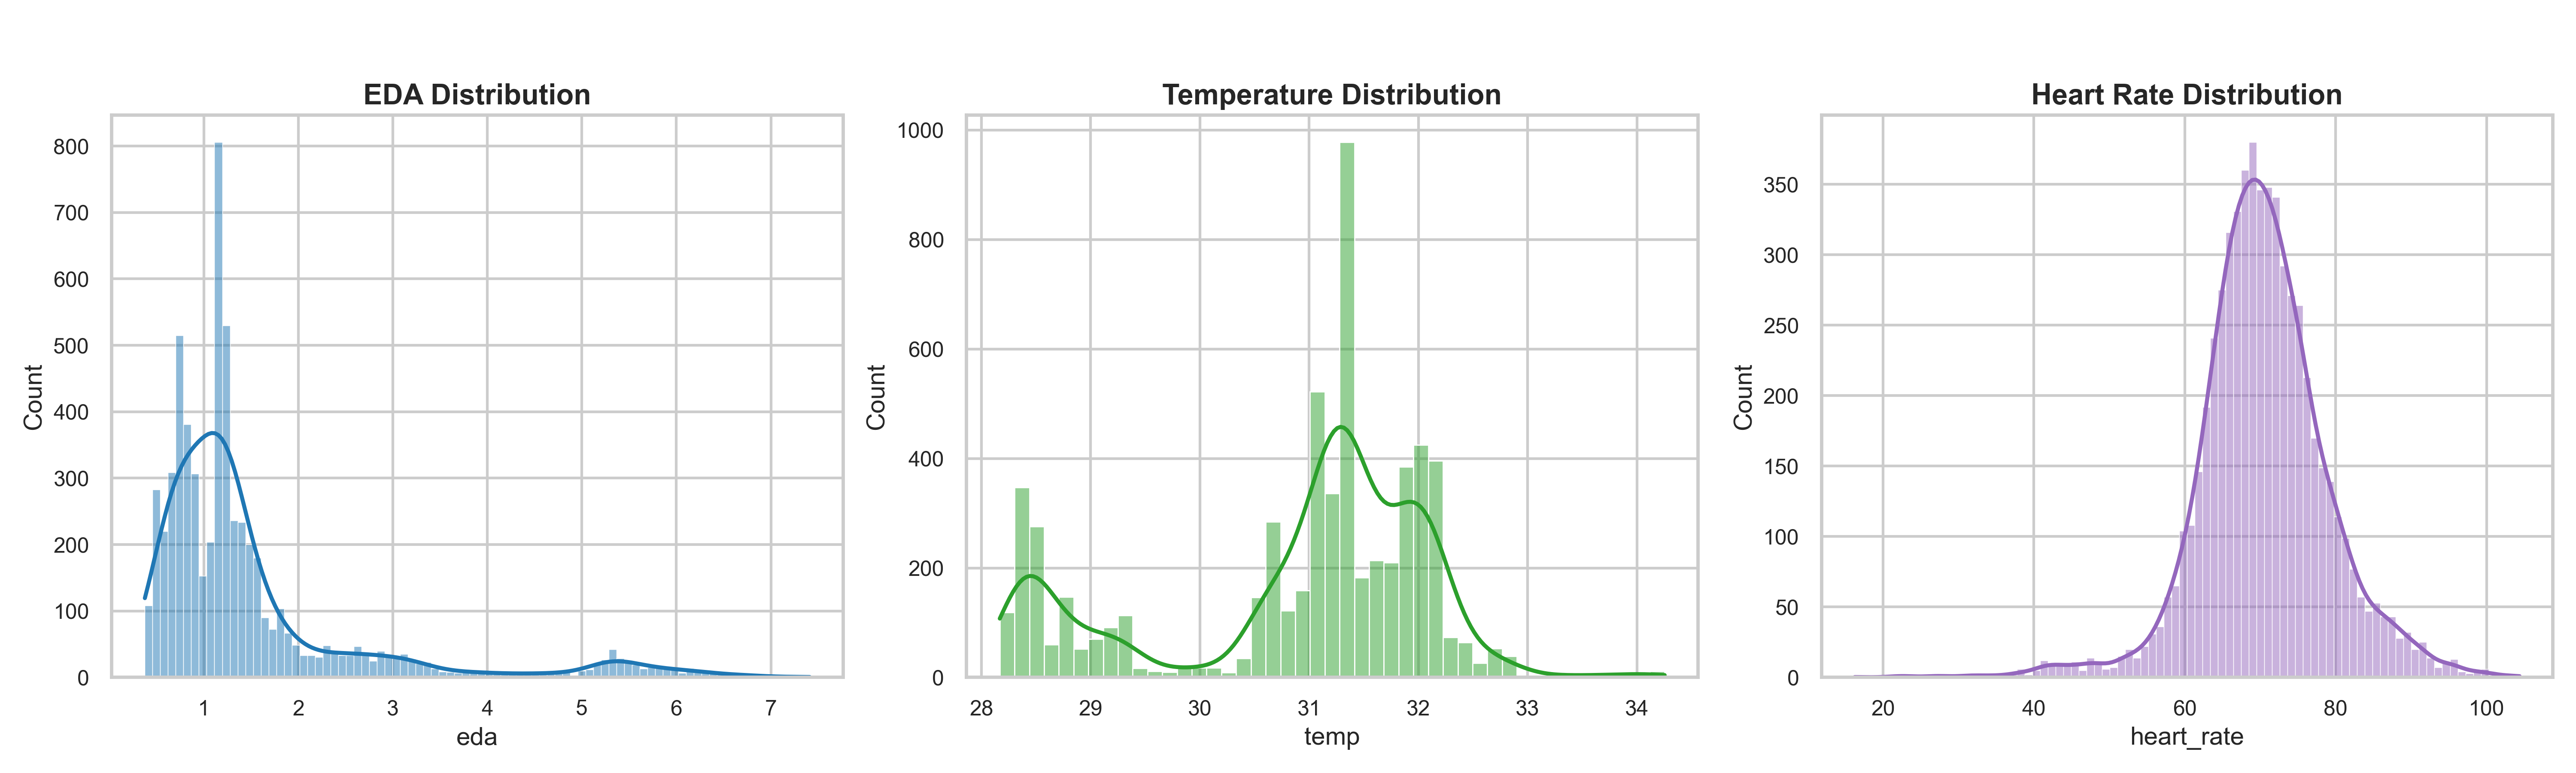
\includegraphics[width=0.95\textwidth]{EDA_Graphs/02_Feature_Density_Analysis.png}
\end{center}
\end{frame}

% ==========================================
% SLIDE 5: CORRELATIONS
% ==========================================
\begin{frame}{Inter-Signal Correlation}
The correlation matrix identifies which features have the strongest linear relationship with the target \textit{Stress Score}.
\vspace{0.2cm}
\begin{columns}
    \begin{column}{0.5\textwidth}
        \centering
        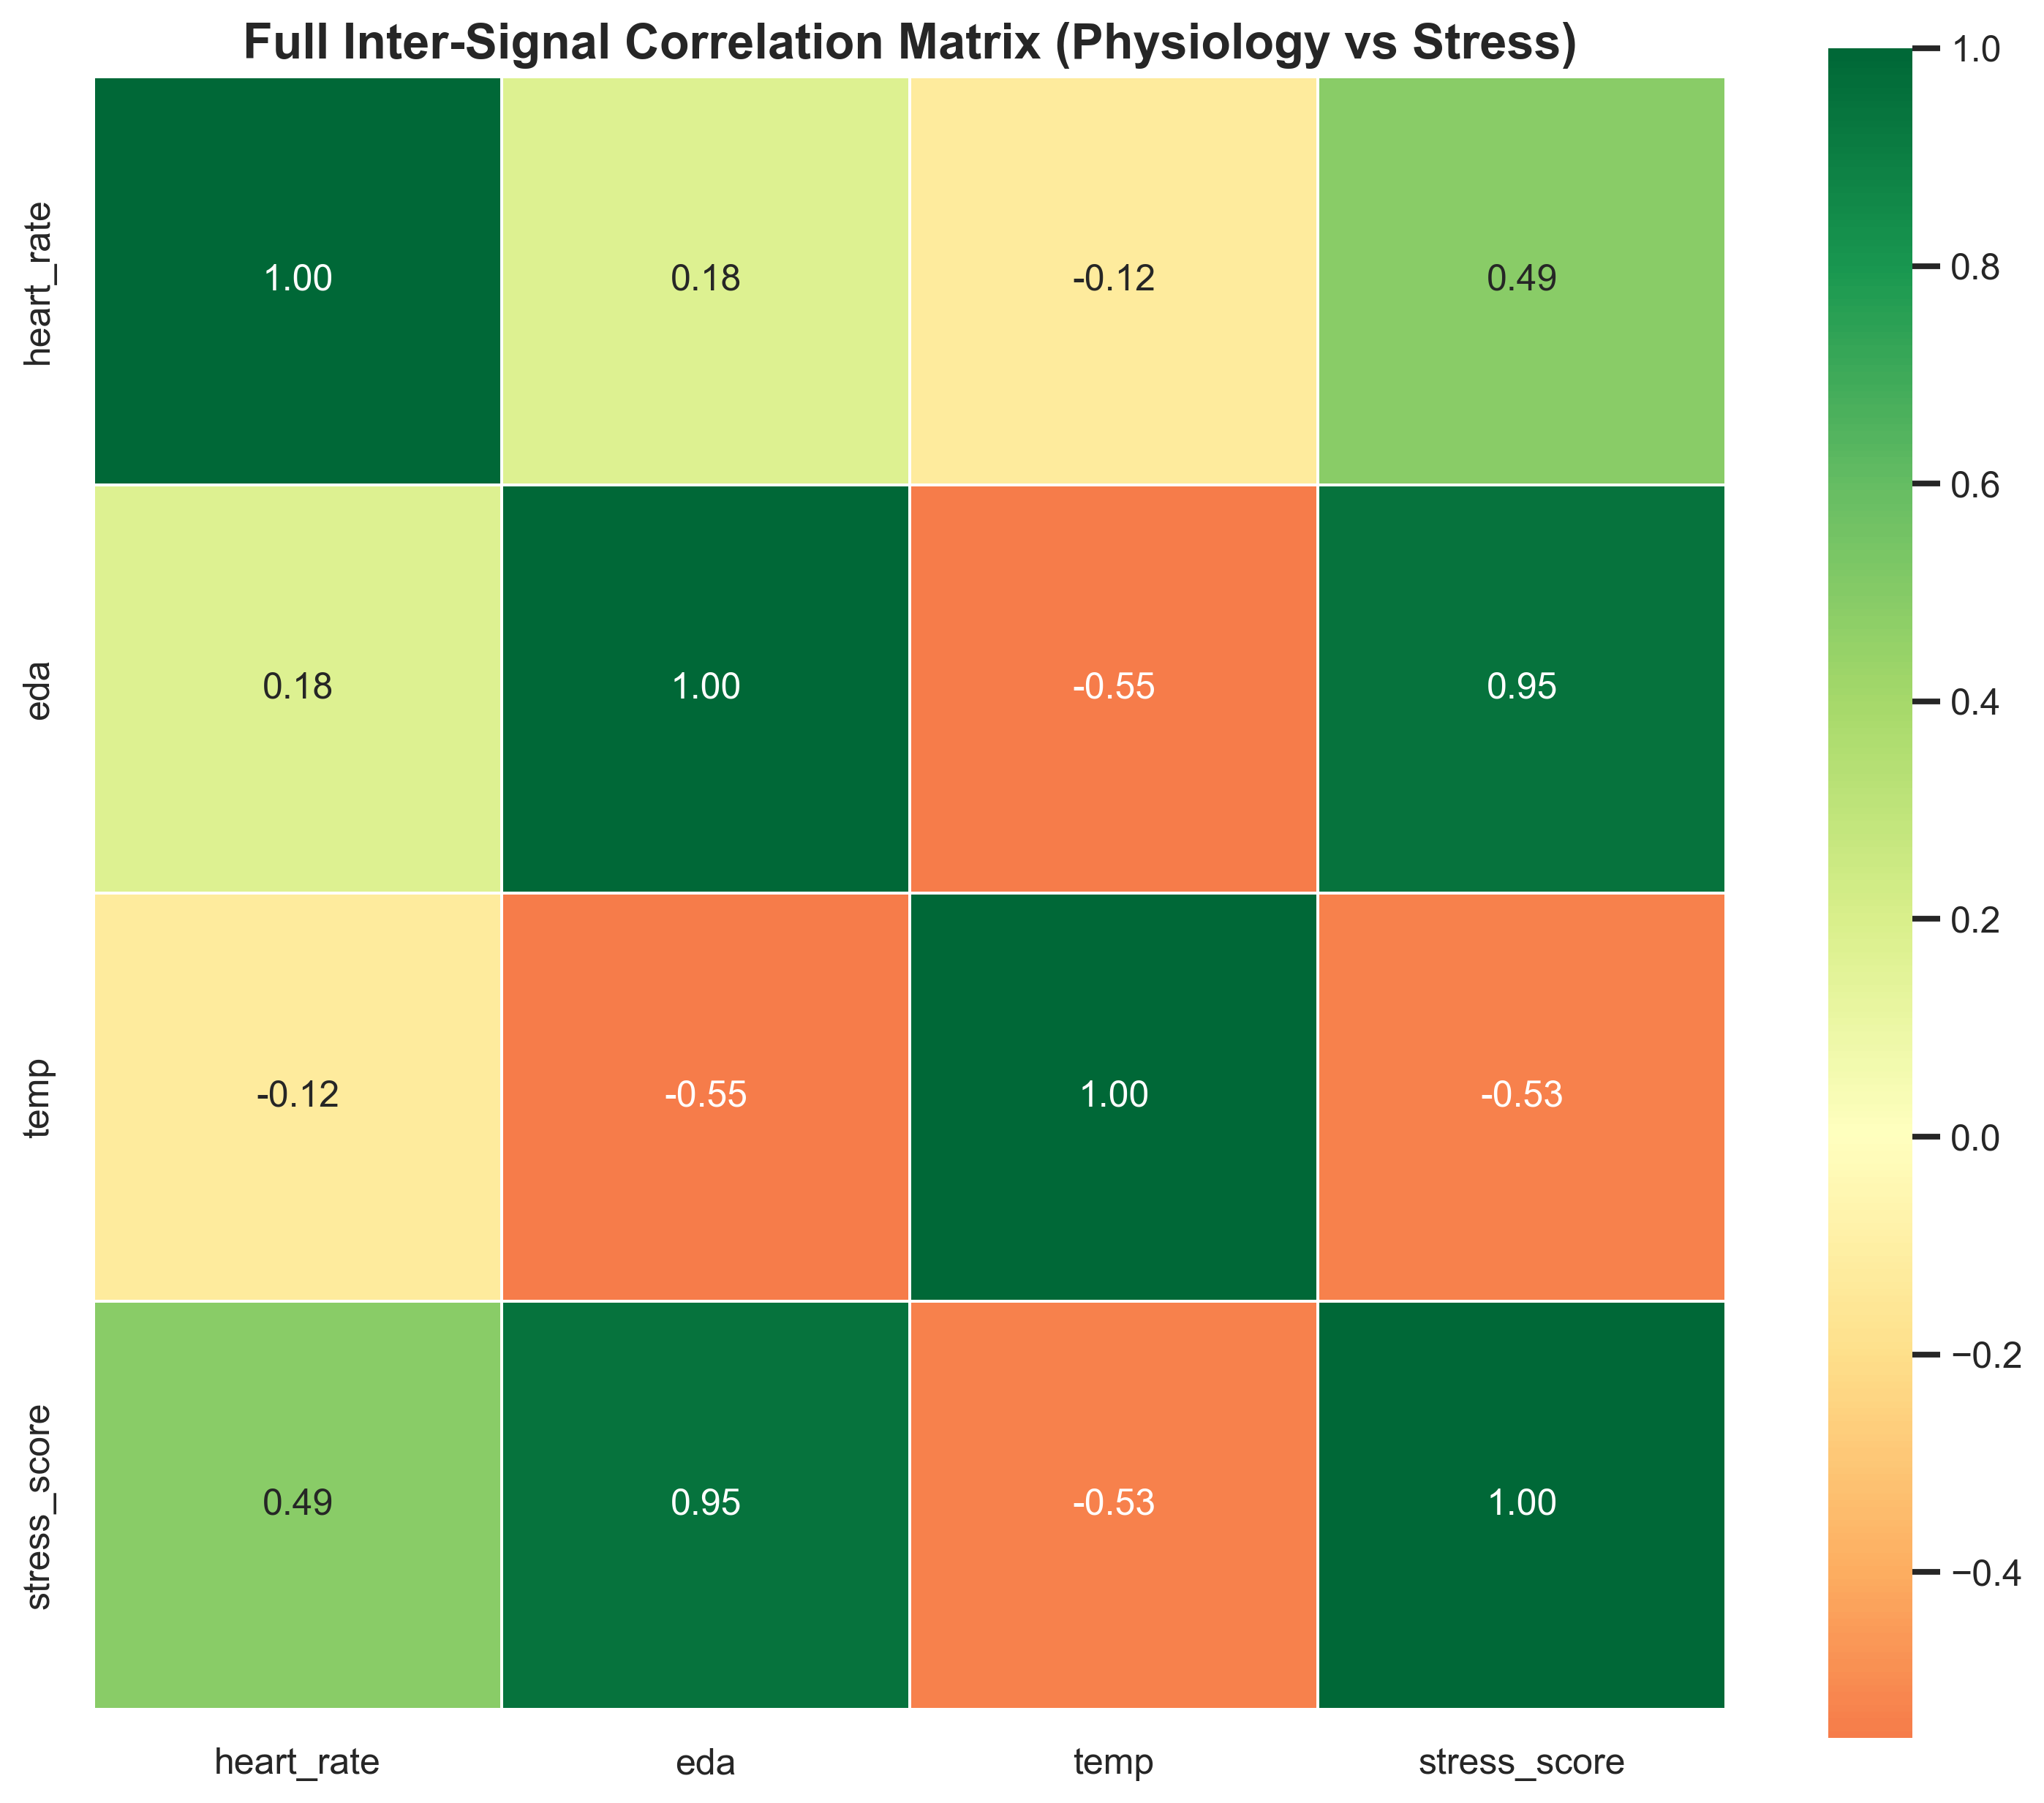
\includegraphics[width=1.0\textwidth]{EDA_Graphs/03_S2_Proper_Correlation.png}
    \end{column}
    \begin{column}{0.45\textwidth}
        \textbf{Observations:}\\[0.2cm]
        \begin{itemize}
            \item \textbf{EDA vs Stress:} Strong positive correlation (0.47). Increased skin conductance directly maps to stress arousal.
            \item \textbf{TEMP vs Stress:} Inverse correlation (-0.29). Peripheral skin temperature typically drops during acute stress.
        \end{itemize}
    \end{column}
\end{columns}
\end{frame}

% ==========================================
% SLIDE 6: SUBJECT DIVERSITY
% ==========================================
\begin{frame}{Dataset Audit: Participant Diversity}
To ensure our pipeline is robust, we audited the physiological profiles of multiple subjects. Stress signatures are highly individual.
\begin{columns}
    \begin{column}{0.48\textwidth}
        \centering
        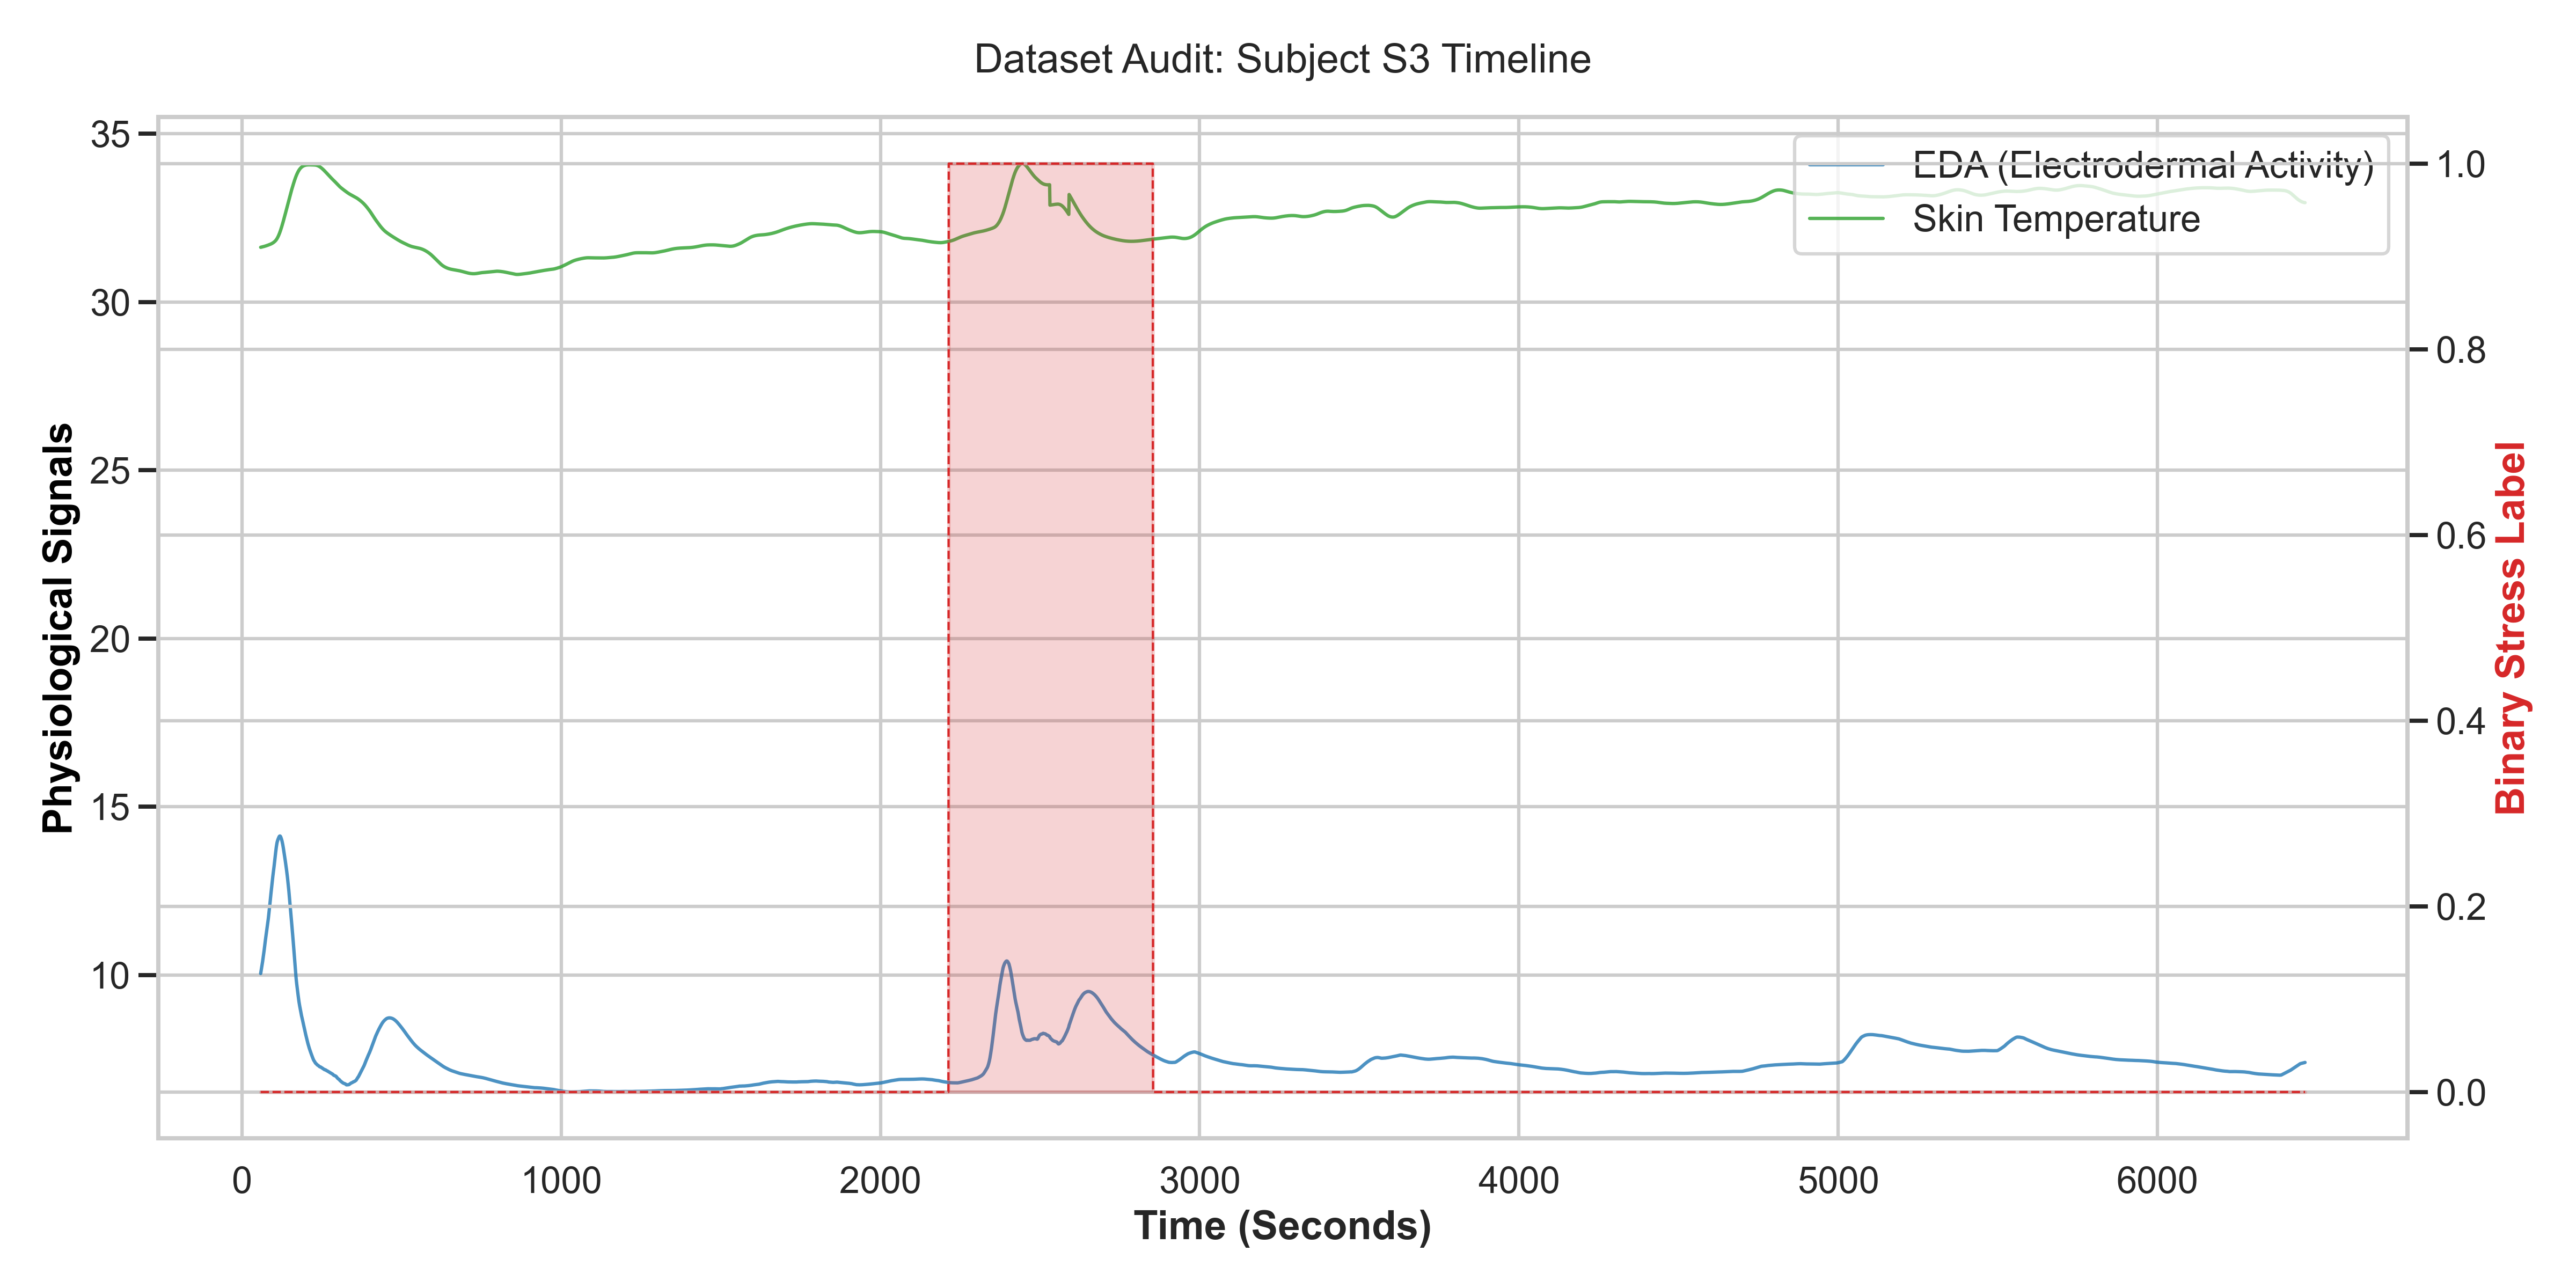
\includegraphics[width=1.0\textwidth]{EDA_Graphs/01_Subject_S3_Timeline.png}
        \small \textit{Subject S3 Profile}
    \end{column}
    \begin{column}{0.48\textwidth}
        \centering
        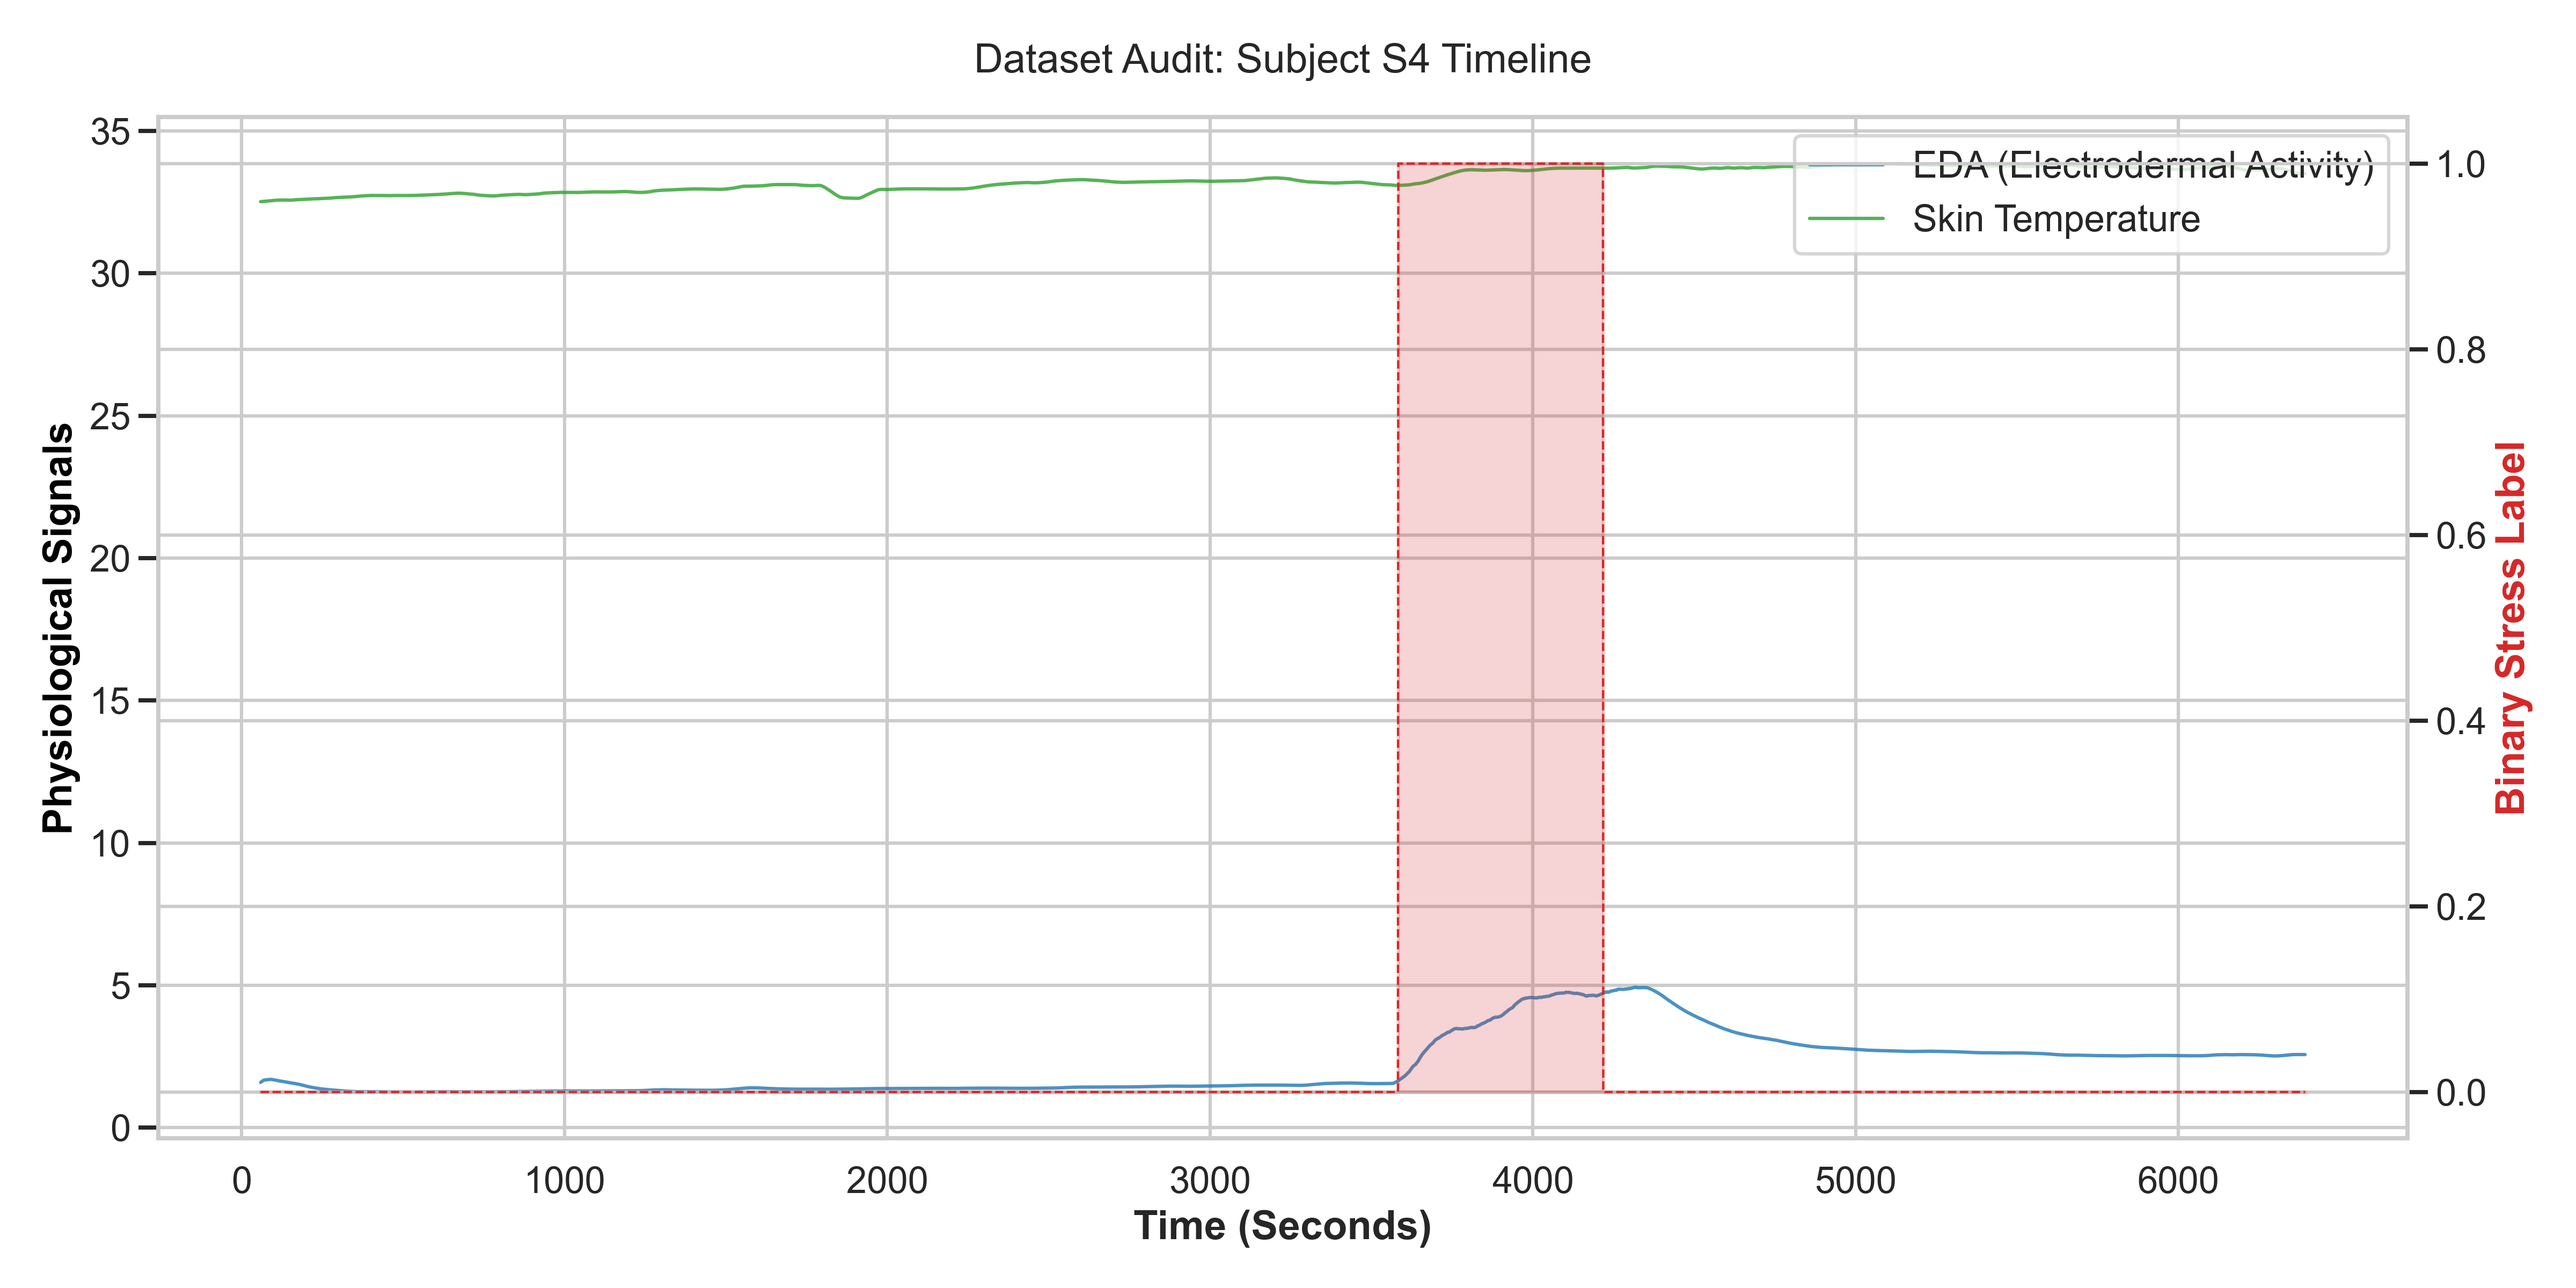
\includegraphics[width=1.0\textwidth]{EDA_Graphs/01_Subject_S4_Timeline.png}
        \small \textit{Subject S4 Profile}
    \end{column}
\end{columns}
\end{frame}

% ==========================================
% SLIDE 7: DEBUGGING BINARY BOX
% ==========================================
\begin{frame}{Debugging Mistake 1: The "Binary Box" Problem}
\begin{columns}
    \begin{column}{0.55\textwidth}
        \textbf{The Error:}\\
        Raw WESAD labels are discrete (Baseline=0, Stress=1). Plotting these creates "rectangular" blocks. 
        \vspace{0.2cm}
        
        \textbf{Why it failed:}
        \begin{itemize}
            \item Zero gradient within blocks.
            \item Statistical models (ARMA/ARIMA) fail to converge on constant signals.
        \end{itemize}
        
        \vspace{0.2cm}
        \textbf{\color{Emerald}The Fix:}\\
        We engineered a \textbf{Continuous Proxy} using rolling density to represent true biological stress intensity (0.0 to 1.0).
    \end{column}
    \begin{column}{0.4\textwidth}
        \centering
        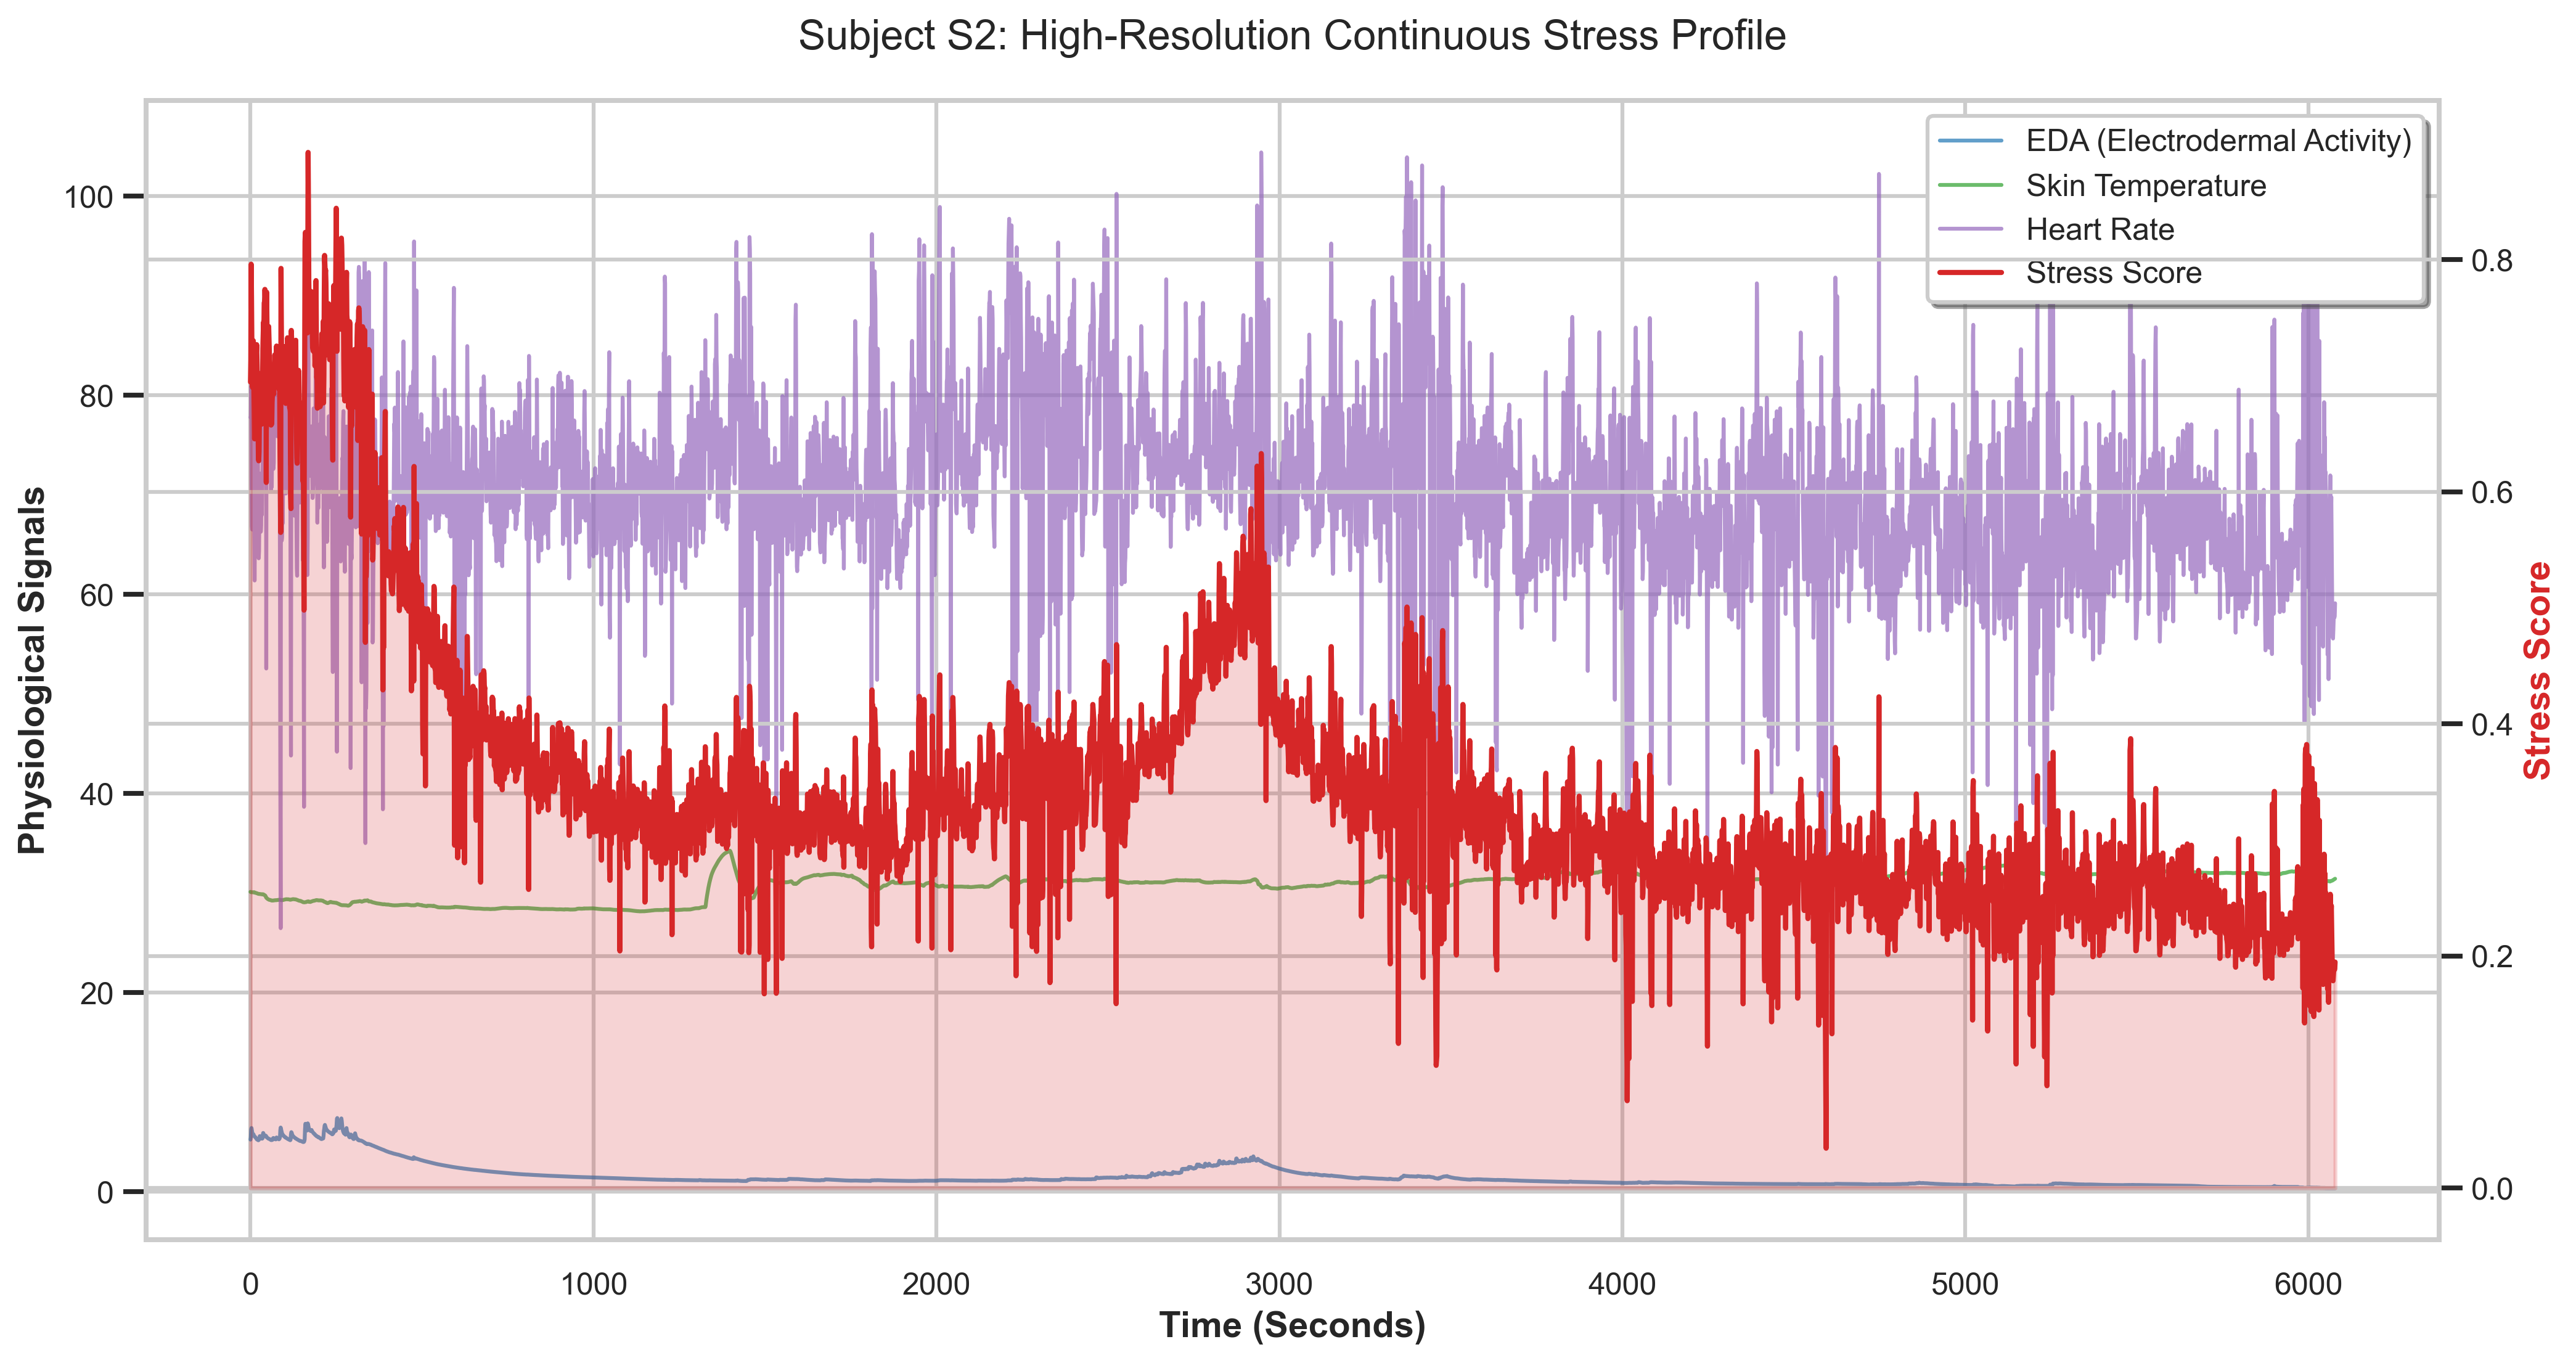
\includegraphics[width=1.0\textwidth]{EDA_Graphs/01_S2_Proper_Timeline.png}
        \small \textit{Fixed Target: Continuous Stress Score}
    \end{column}
\end{columns}
\end{frame}

% ==========================================
% SLIDE 8: DEBUGGING LEAKAGE
% ==========================================
\begin{frame}{Debugging Mistake 2: Systemic Data Leakage}
\begin{columns}
    \begin{column}{0.5\textwidth}
        \textbf{The Illusion of High Accuracy:}\\
        Early iterations used Heart Rate at time $t$ to predict Stress at time $t$. Because HR and Stress occur simultaneously, the model was "cheating" rather than forecasting.
        
        \vspace{0.4cm}
        \textbf{\color{Emerald}The Strict $t-1$ Lag Policy:}\\
        All exogenous signals (HR, EDA, TEMP) were explicitly shifted backwards. 
    \end{column}
    \begin{column}{0.45\textwidth}
        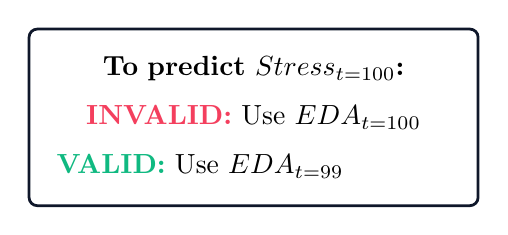
\begin{tikzpicture}
            \node[fill=white, draw=Navy, line width=1pt, rounded corners=3pt, inner sep=10pt, text width=5cm] {
                \centering
                \textbf{To predict $Stress_{t=100}$:}\\
                \vspace{0.2cm}
                \textcolor{Coral}{\textbf{INVALID:}} Use $EDA_{t=100}$\\
                \vspace{0.2cm}
                \textcolor{Emerald}{\textbf{VALID:}} Use $EDA_{t=99}$
            };
        \end{tikzpicture}
        \vspace{0.3cm}\\
        \textit{This forces the model to predict the future based strictly on historical evidence.}
    \end{column}
\end{columns}
\end{frame}

% ==========================================
% SLIDE 9: STATIONARITY
% ==========================================
\begin{frame}{Debugging Mistake 3: Non-Stationarity ($d=1$)}
Time-series models require a stable mean and variance. ADF tests on the raw stress score yielded $p=0.066$ (Non-Stationary). 
\vspace{0.2cm}
\begin{columns}
    \begin{column}{0.55\textwidth}
        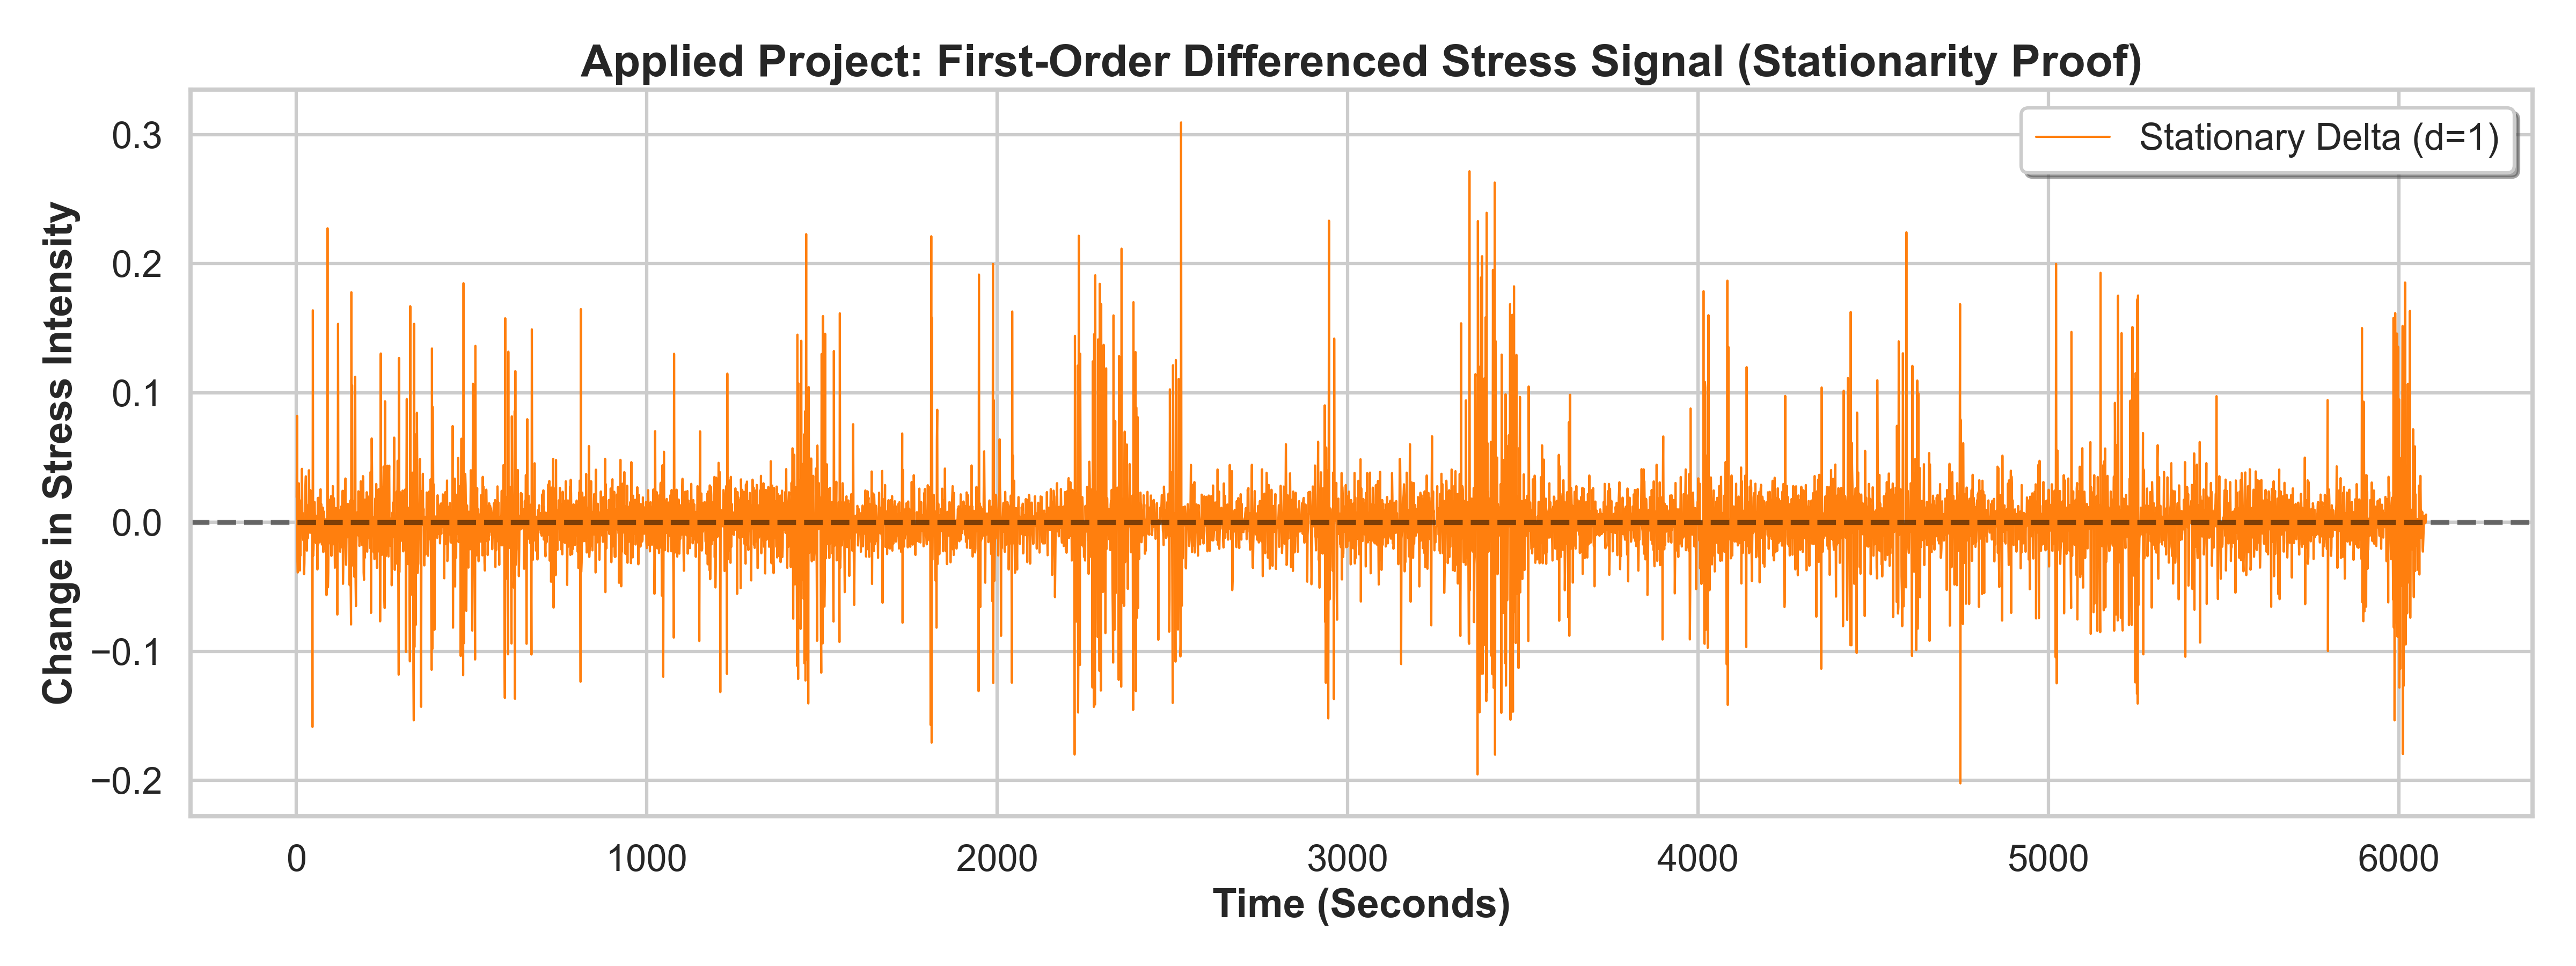
\includegraphics[width=1.0\textwidth]{EDA_Graphs/05_Differenced_Signal_Timeline.png}
    \end{column}
    \begin{column}{0.4\textwidth}
        \textbf{\color{Emerald}First-Order Differencing}\\
        We transformed the target into $\Delta y_t = y_t - y_{t-1}$.
        \vspace{0.2cm}
        \begin{itemize}
            \item \textbf{New $p$-value:} $0.000$
            \item \textbf{Result:} Perfect Stationarity.
            \item Required for ARMA, ARIMA, and SARIMA models.
        \end{itemize}
    \end{column}
\end{columns}
\end{frame}

% ==========================================
% SLIDE 10: MEMORY DIAGNOSTICS
% ==========================================
\begin{frame}{Statistical Memory Diagnostics (ACF \& PACF)}
To identify the theoretical bounds for our AR and MA models, we analyzed the Autocorrelation patterns of the stationary signal.
\begin{center}
    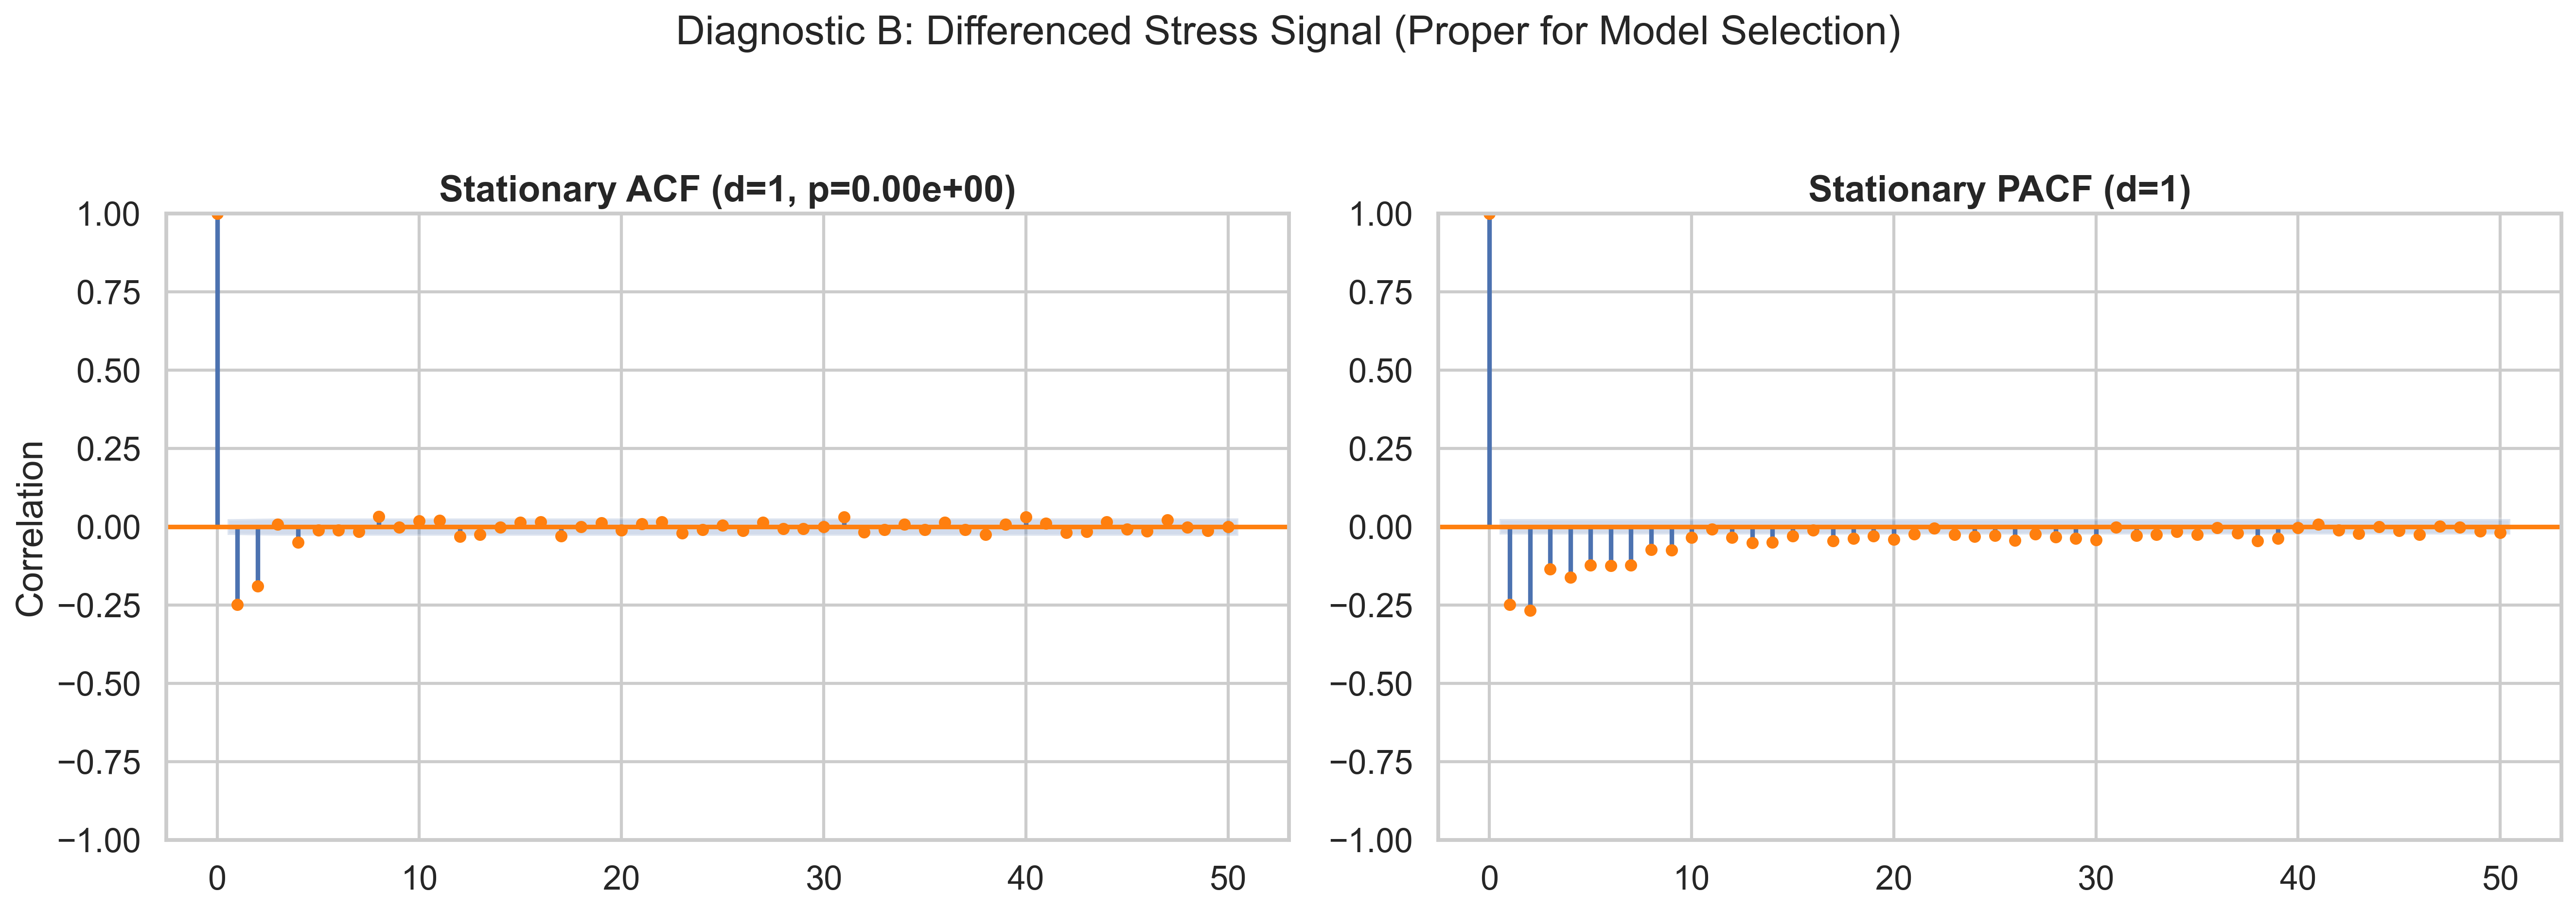
\includegraphics[width=0.9\textwidth]{EDA_Graphs/06_Stationary_Lag_Diagnostics.png}
\end{center}
\textbf{Findings:} The sharp PACF cut-off dictated an AR parameter of $p=2$, while ACF suggested an MA component of $q=3$.
\end{frame}

% ==========================================
% SLIDE 11: ROLL FORWARD STRATEGY
% ==========================================
\begin{frame}{Evaluation Protocol: Walk-Forward Validation}
\textbf{Why an 80/20 static split fails for High-Frequency Series:}\\
A model trained on the first 80\% of data loses its "memory" when predicting the very end of the test set, leading to massive decay.
\vspace{0.4cm}

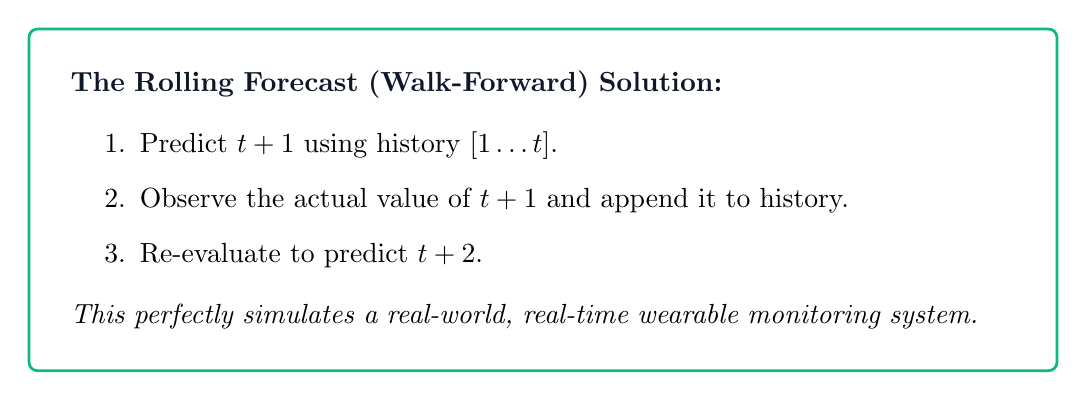
\begin{tikzpicture}
    \node[fill=white, draw=Emerald, line width=1pt, rounded corners=3pt, inner sep=15pt, text width=12cm] {
        \textbf{\color{Navy}The Rolling Forecast (Walk-Forward) Solution:}\\[0.2cm]
        \begin{enumerate}
            \item Predict $t+1$ using history $[1 \dots t]$.
            \item Observe the actual value of $t+1$ and append it to history.
            \item Re-evaluate to predict $t+2$.
        \end{enumerate}
        \textit{This perfectly simulates a real-world, real-time wearable monitoring system.}
    };
\end{tikzpicture}
\end{frame}

% ==========================================
% MODEL SLIDES
% ==========================================
\begin{frame}{Model 1: Naive Persistence (The Baseline)}
\begin{columns}
    \begin{column}{0.65\textwidth}
        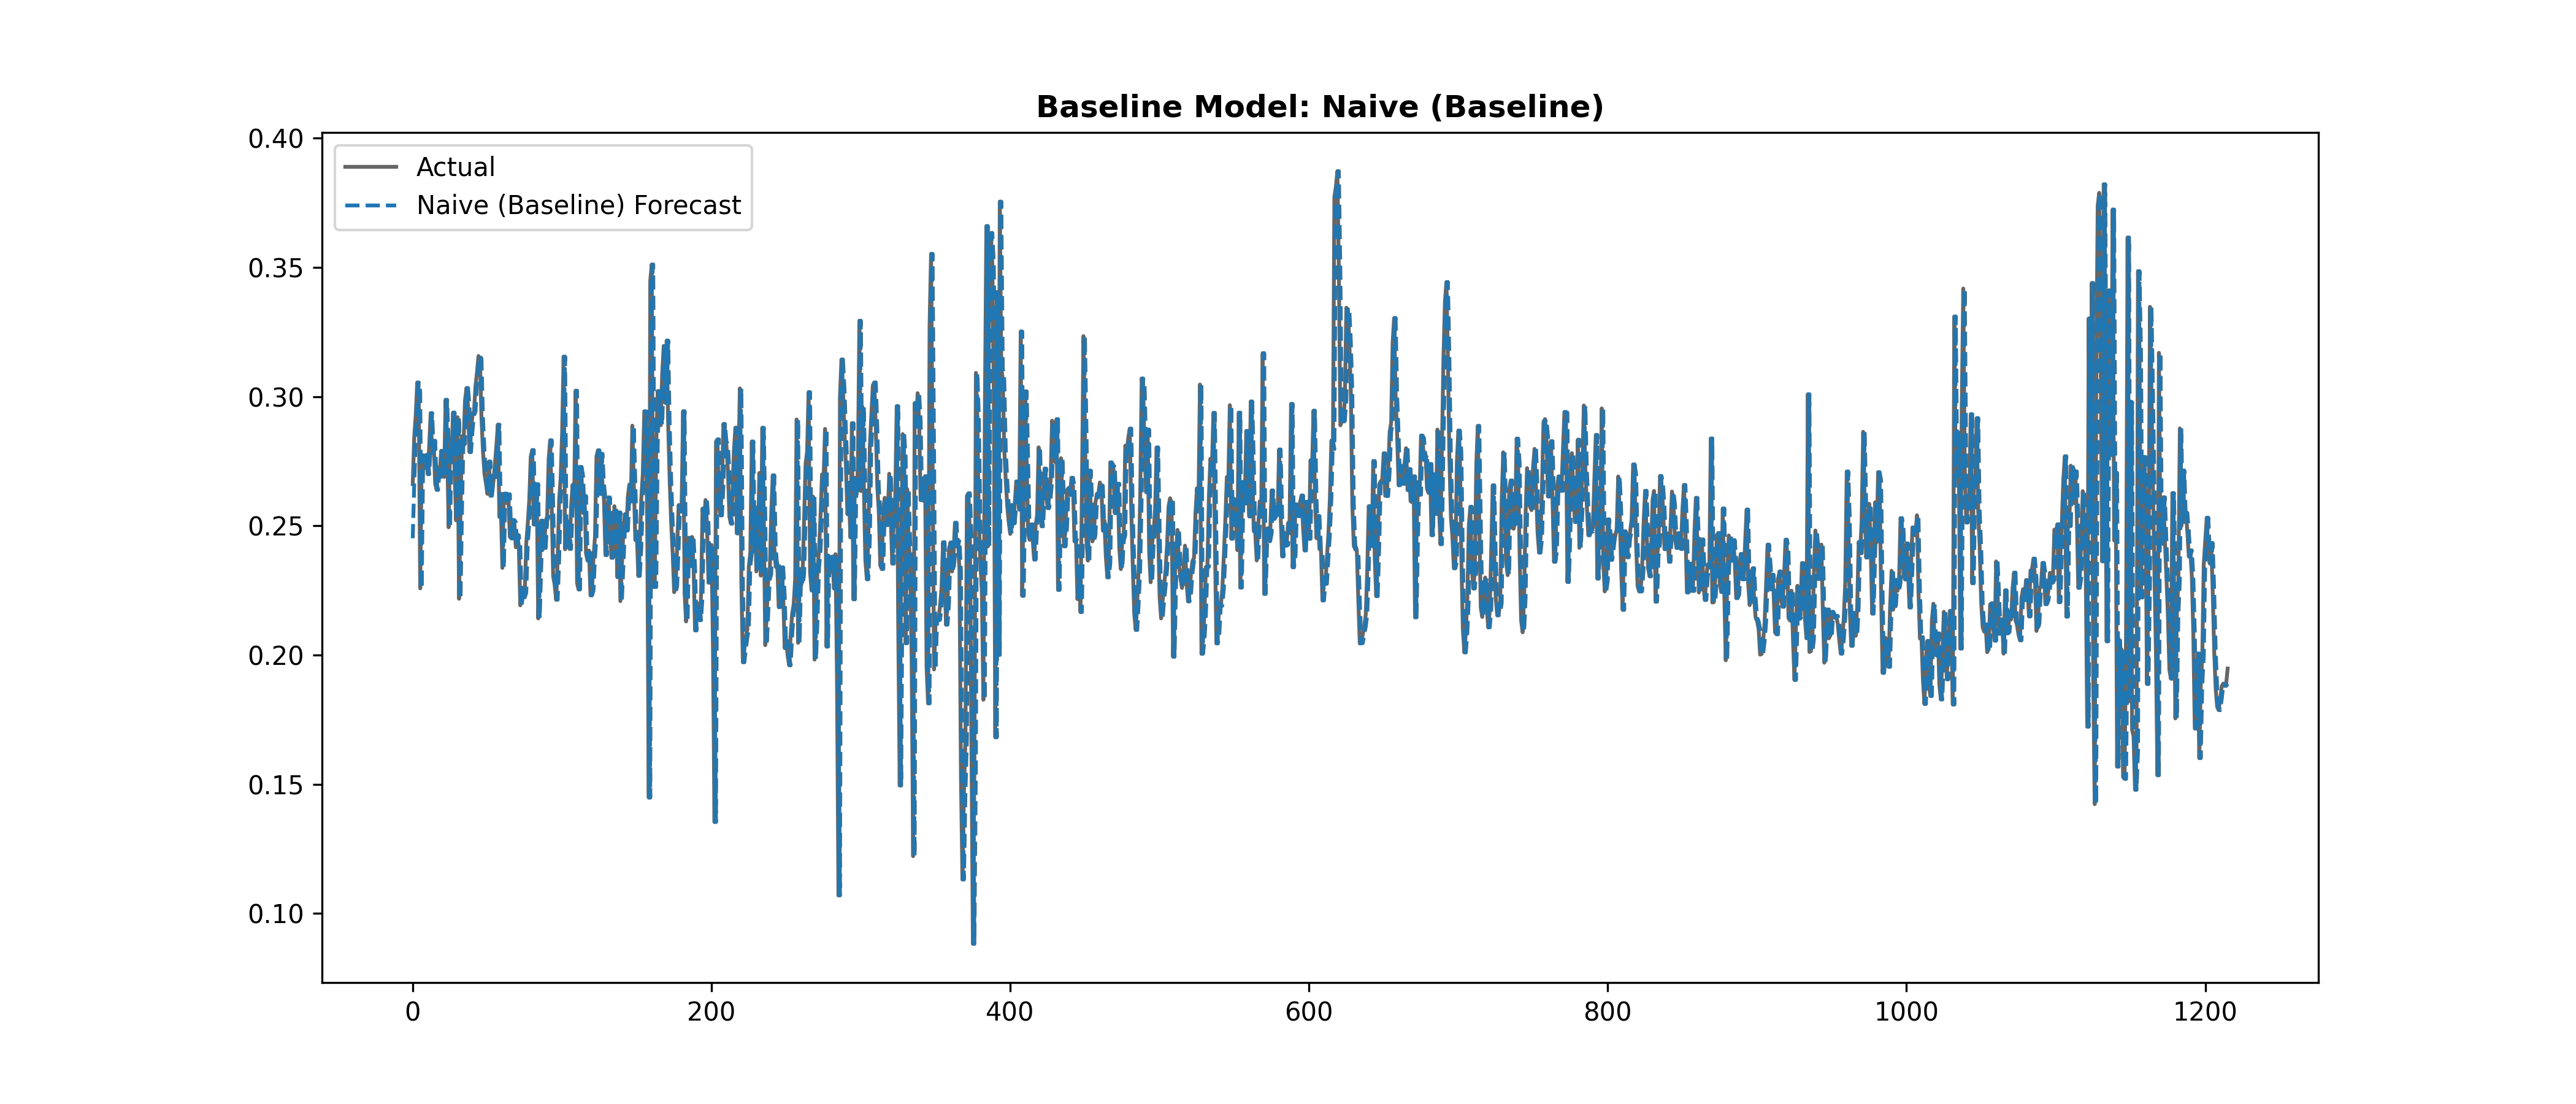
\includegraphics[width=1.0\textwidth]{Forecasting_Graphs/00_Naive_(Baseline).png}
    \end{column}
    \begin{column}{0.3\textwidth}
        \textbf{Theory:}\\
        Assumes current state dictates the future: $\hat{y}_{t+1} = y_t$\\[0.4cm]
        \slidemetrics{Naive}{0.0211}{0.0345}{8.68}{0.0673}
    \end{column}
\end{columns}
\end{frame}

\begin{frame}{Model 2: Simple Moving Average (SMA)}
\begin{columns}
    \begin{column}{0.65\textwidth}
        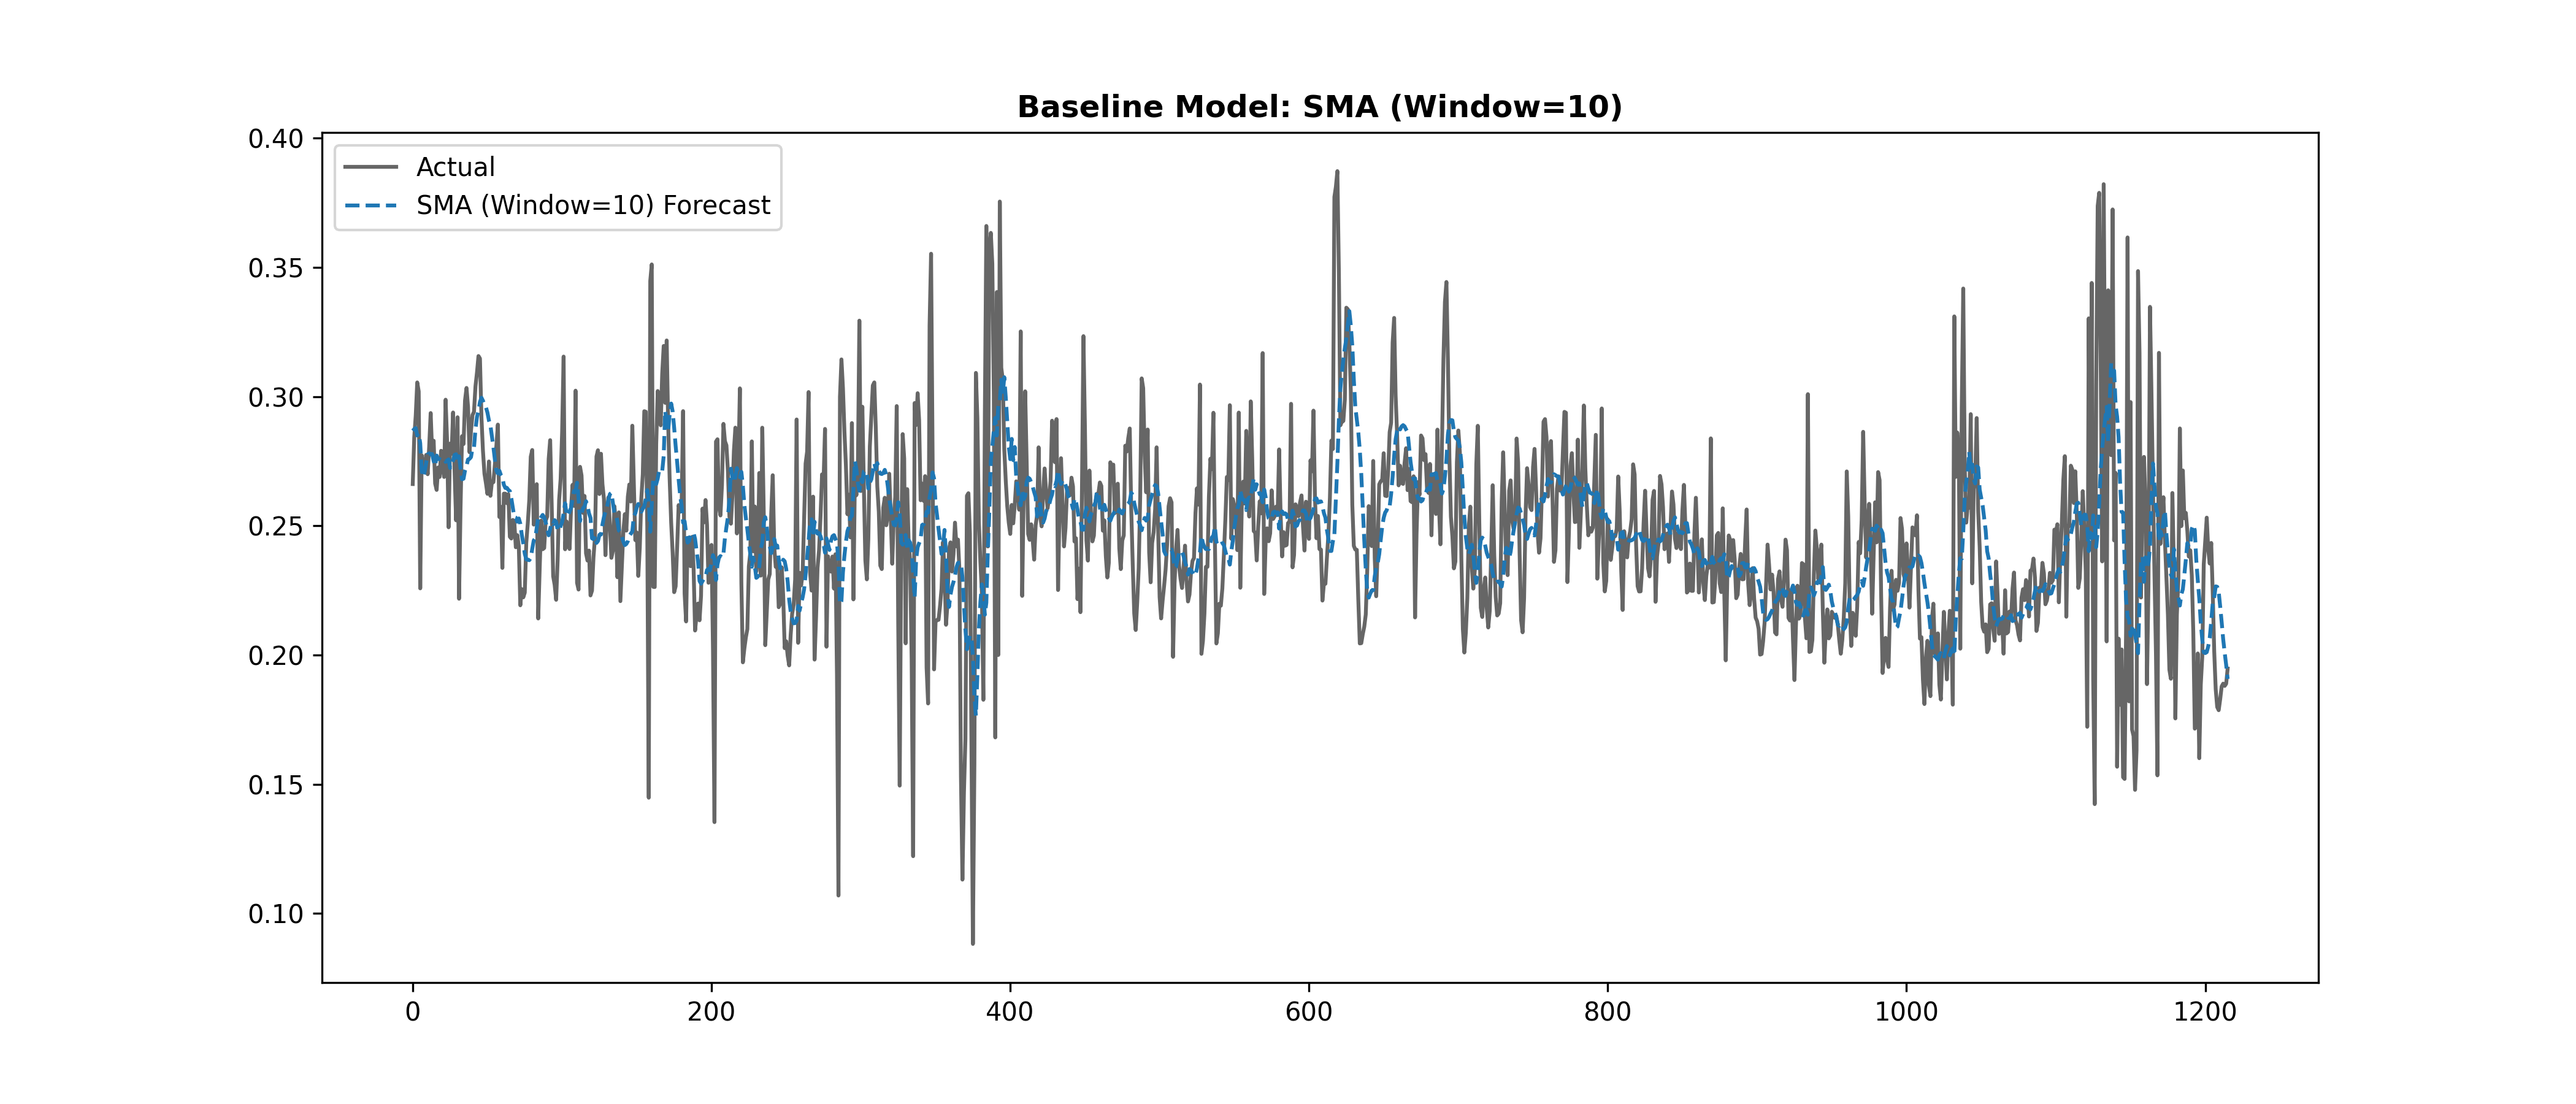
\includegraphics[width=1.0\textwidth]{Forecasting_Graphs/00_SMA_(Window=10).png}
    \end{column}
    \begin{column}{0.3\textwidth}
        \textbf{Theory:}\\
        Averages last 10s to smooth high-frequency sensor noise.\\[0.4cm]
        \slidemetrics{SMA-10}{0.0229}{0.0326}{9.62}{0.1716}
    \end{column}
\end{columns}
\end{frame}

\begin{frame}{Model 3: AutoRegressive (AR)}
\begin{columns}
    \begin{column}{0.65\textwidth}
        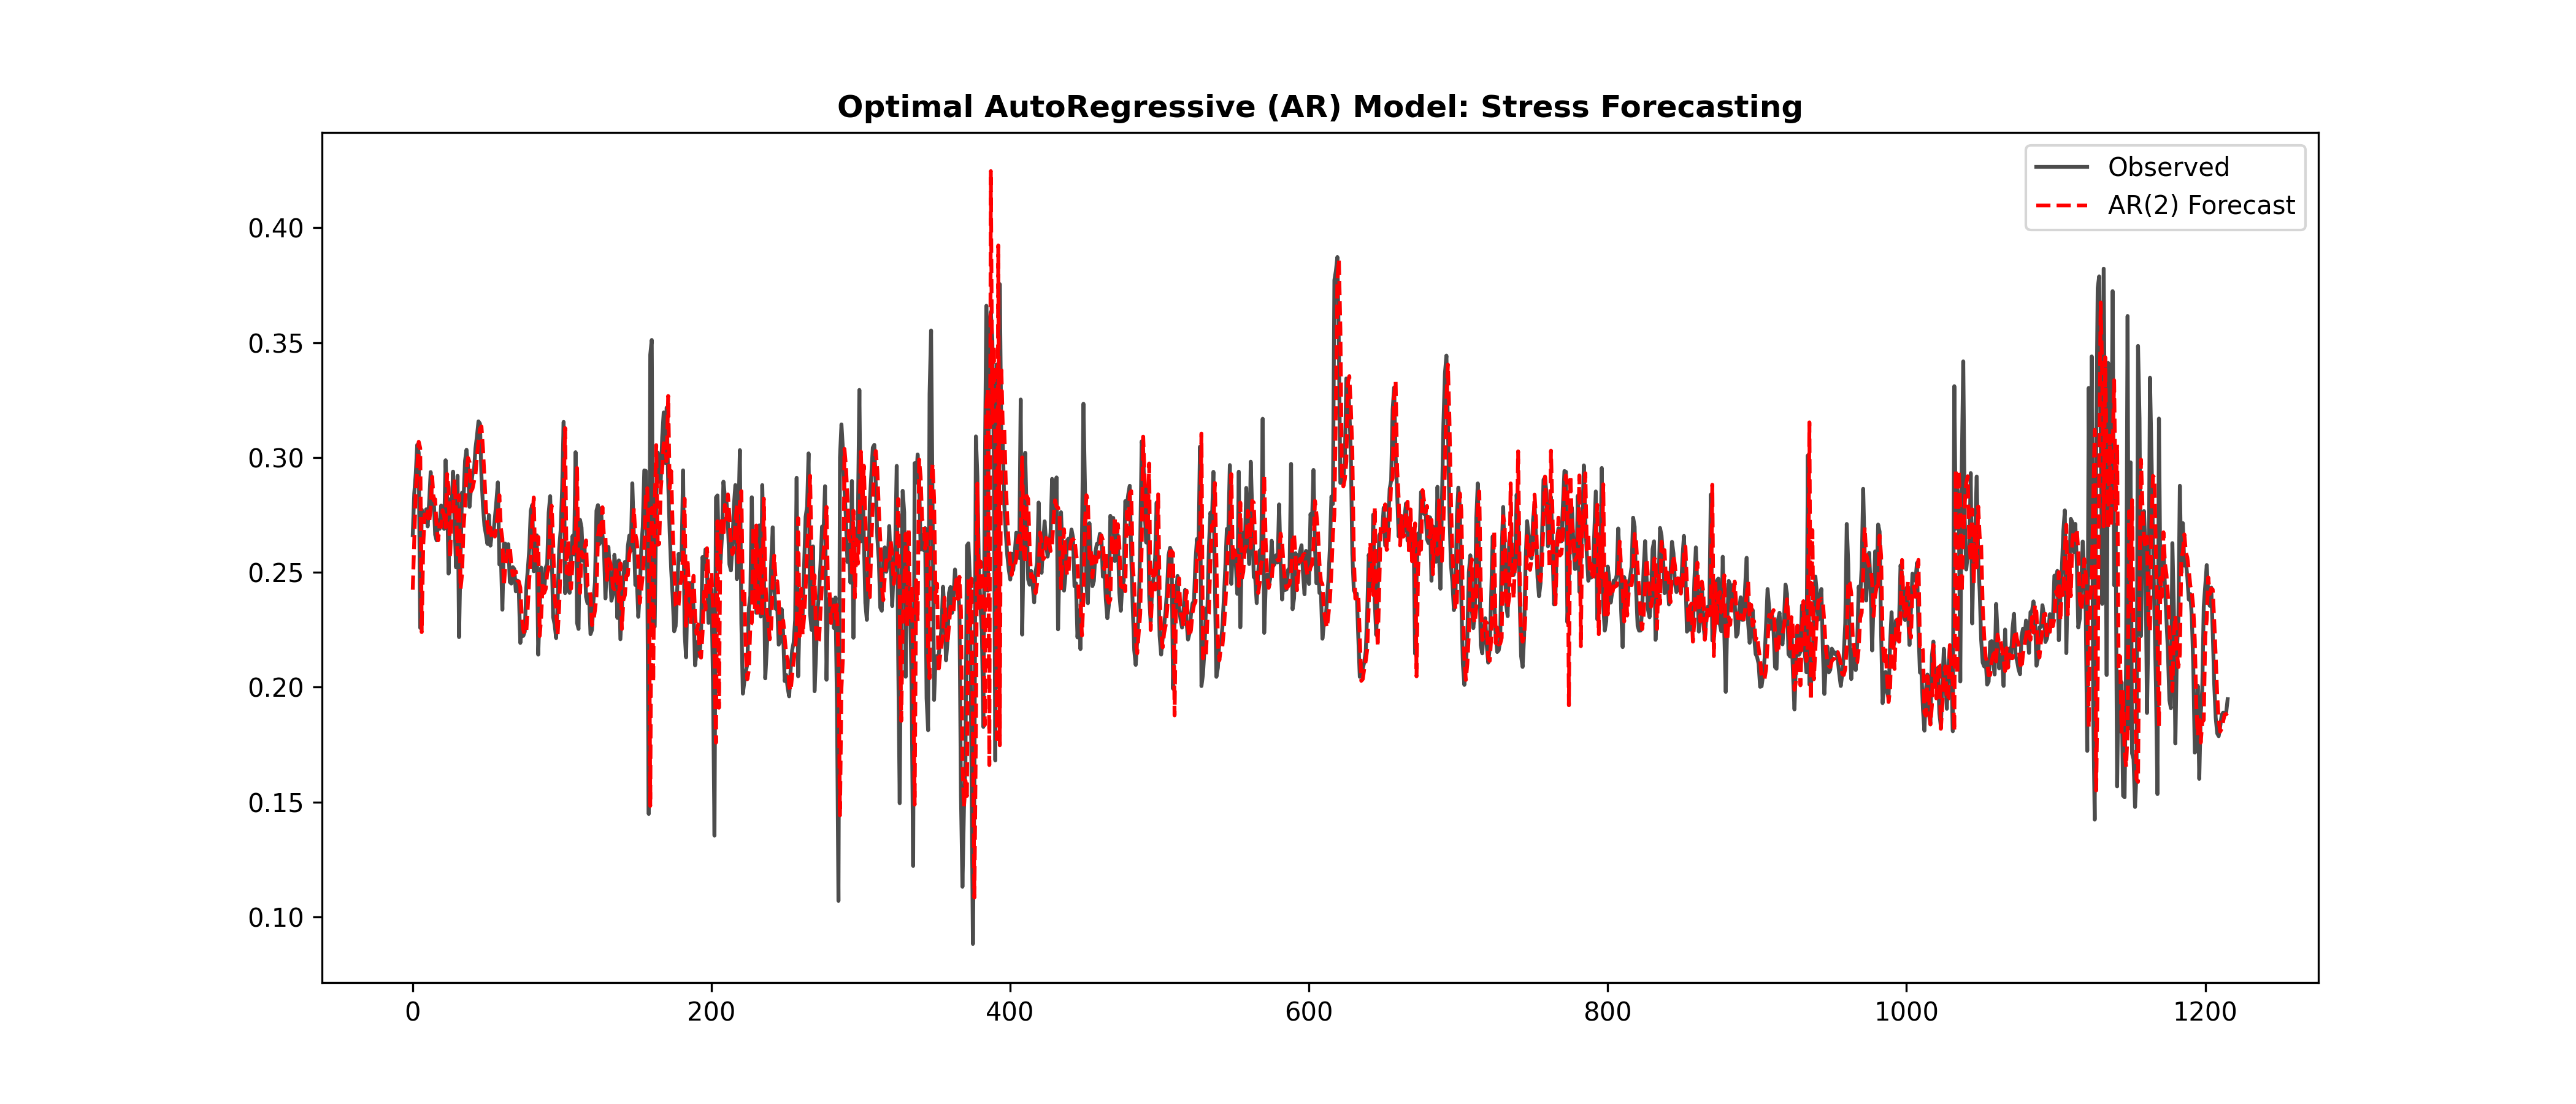
\includegraphics[width=1.0\textwidth]{Forecasting_Graphs/03_AR_Optimized.png}
    \end{column}
    \begin{column}{0.3\textwidth}
        \textbf{Theory:}\\
        Linear function of its own $p=2$ lags to capture momentum.\\[0.4cm]
        \slidemetrics{AR(2)}{0.0210}{0.0342}{8.66}{0.0840}
    \end{column}
\end{columns}
\end{frame}

\begin{frame}{Model 4: Moving Average (MA)}
\begin{columns}
    \begin{column}{0.65\textwidth}
        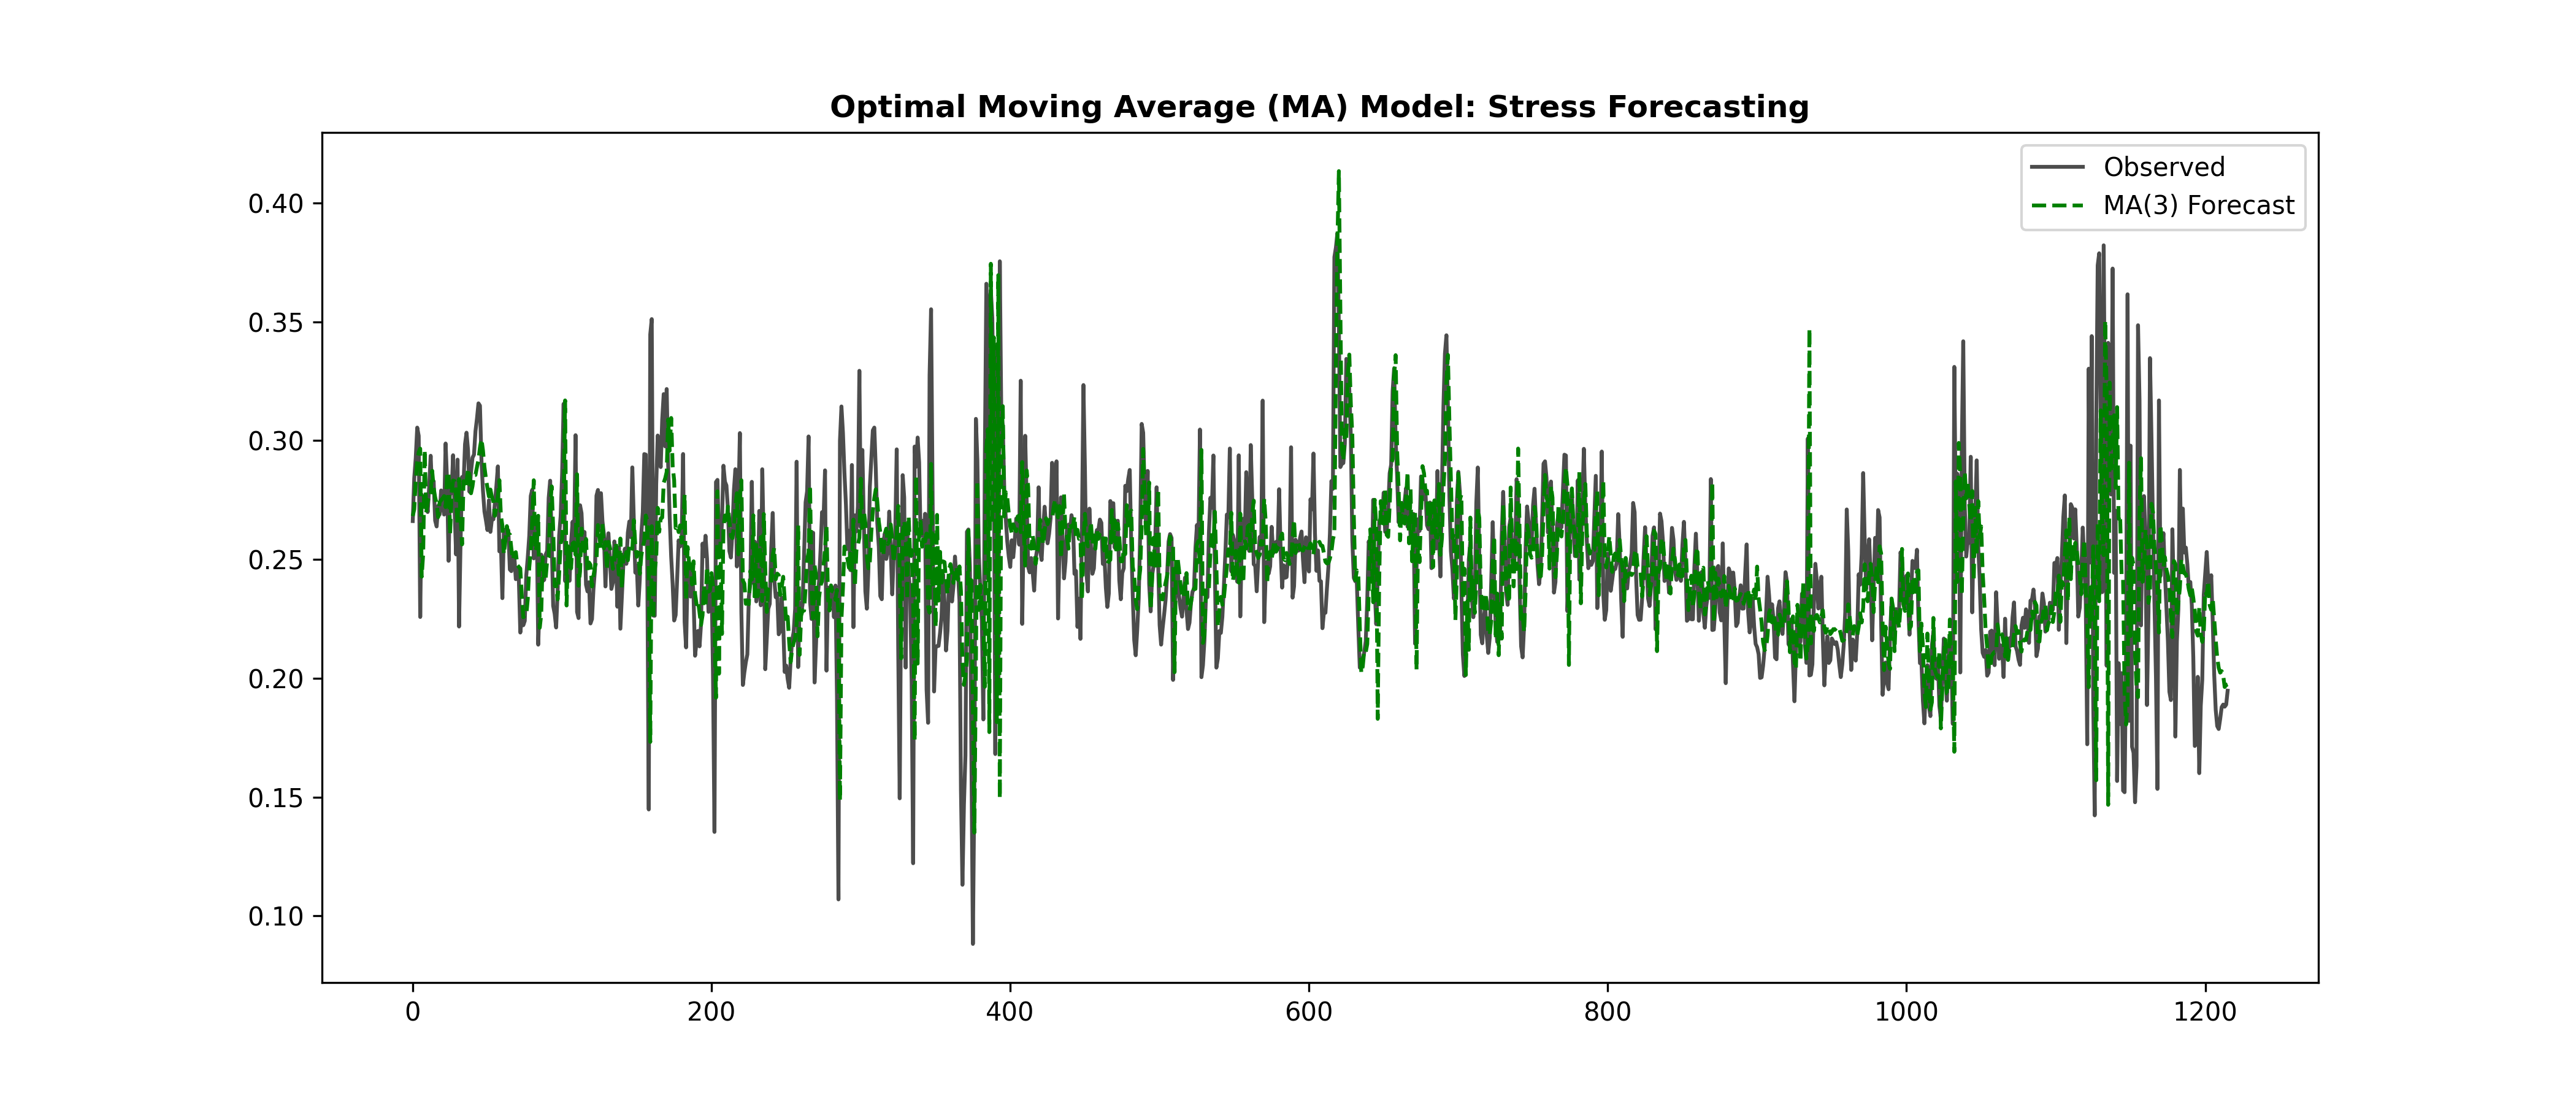
\includegraphics[width=1.0\textwidth]{Forecasting_Graphs/04_MA_Optimized.png}
    \end{column}
    \begin{column}{0.3\textwidth}
        \textbf{Theory:}\\
        Uses past forecast errors ($q=3$) to correct for sudden physiological "shocks".\\[0.4cm]
        \slidemetrics{MA(3)}{0.0209}{0.0335}{8.72}{0.1236}
    \end{column}
\end{columns}
\end{frame}

\begin{frame}{Model 5: ARMA(2,3)}
\begin{columns}
    \begin{column}{0.65\textwidth}
        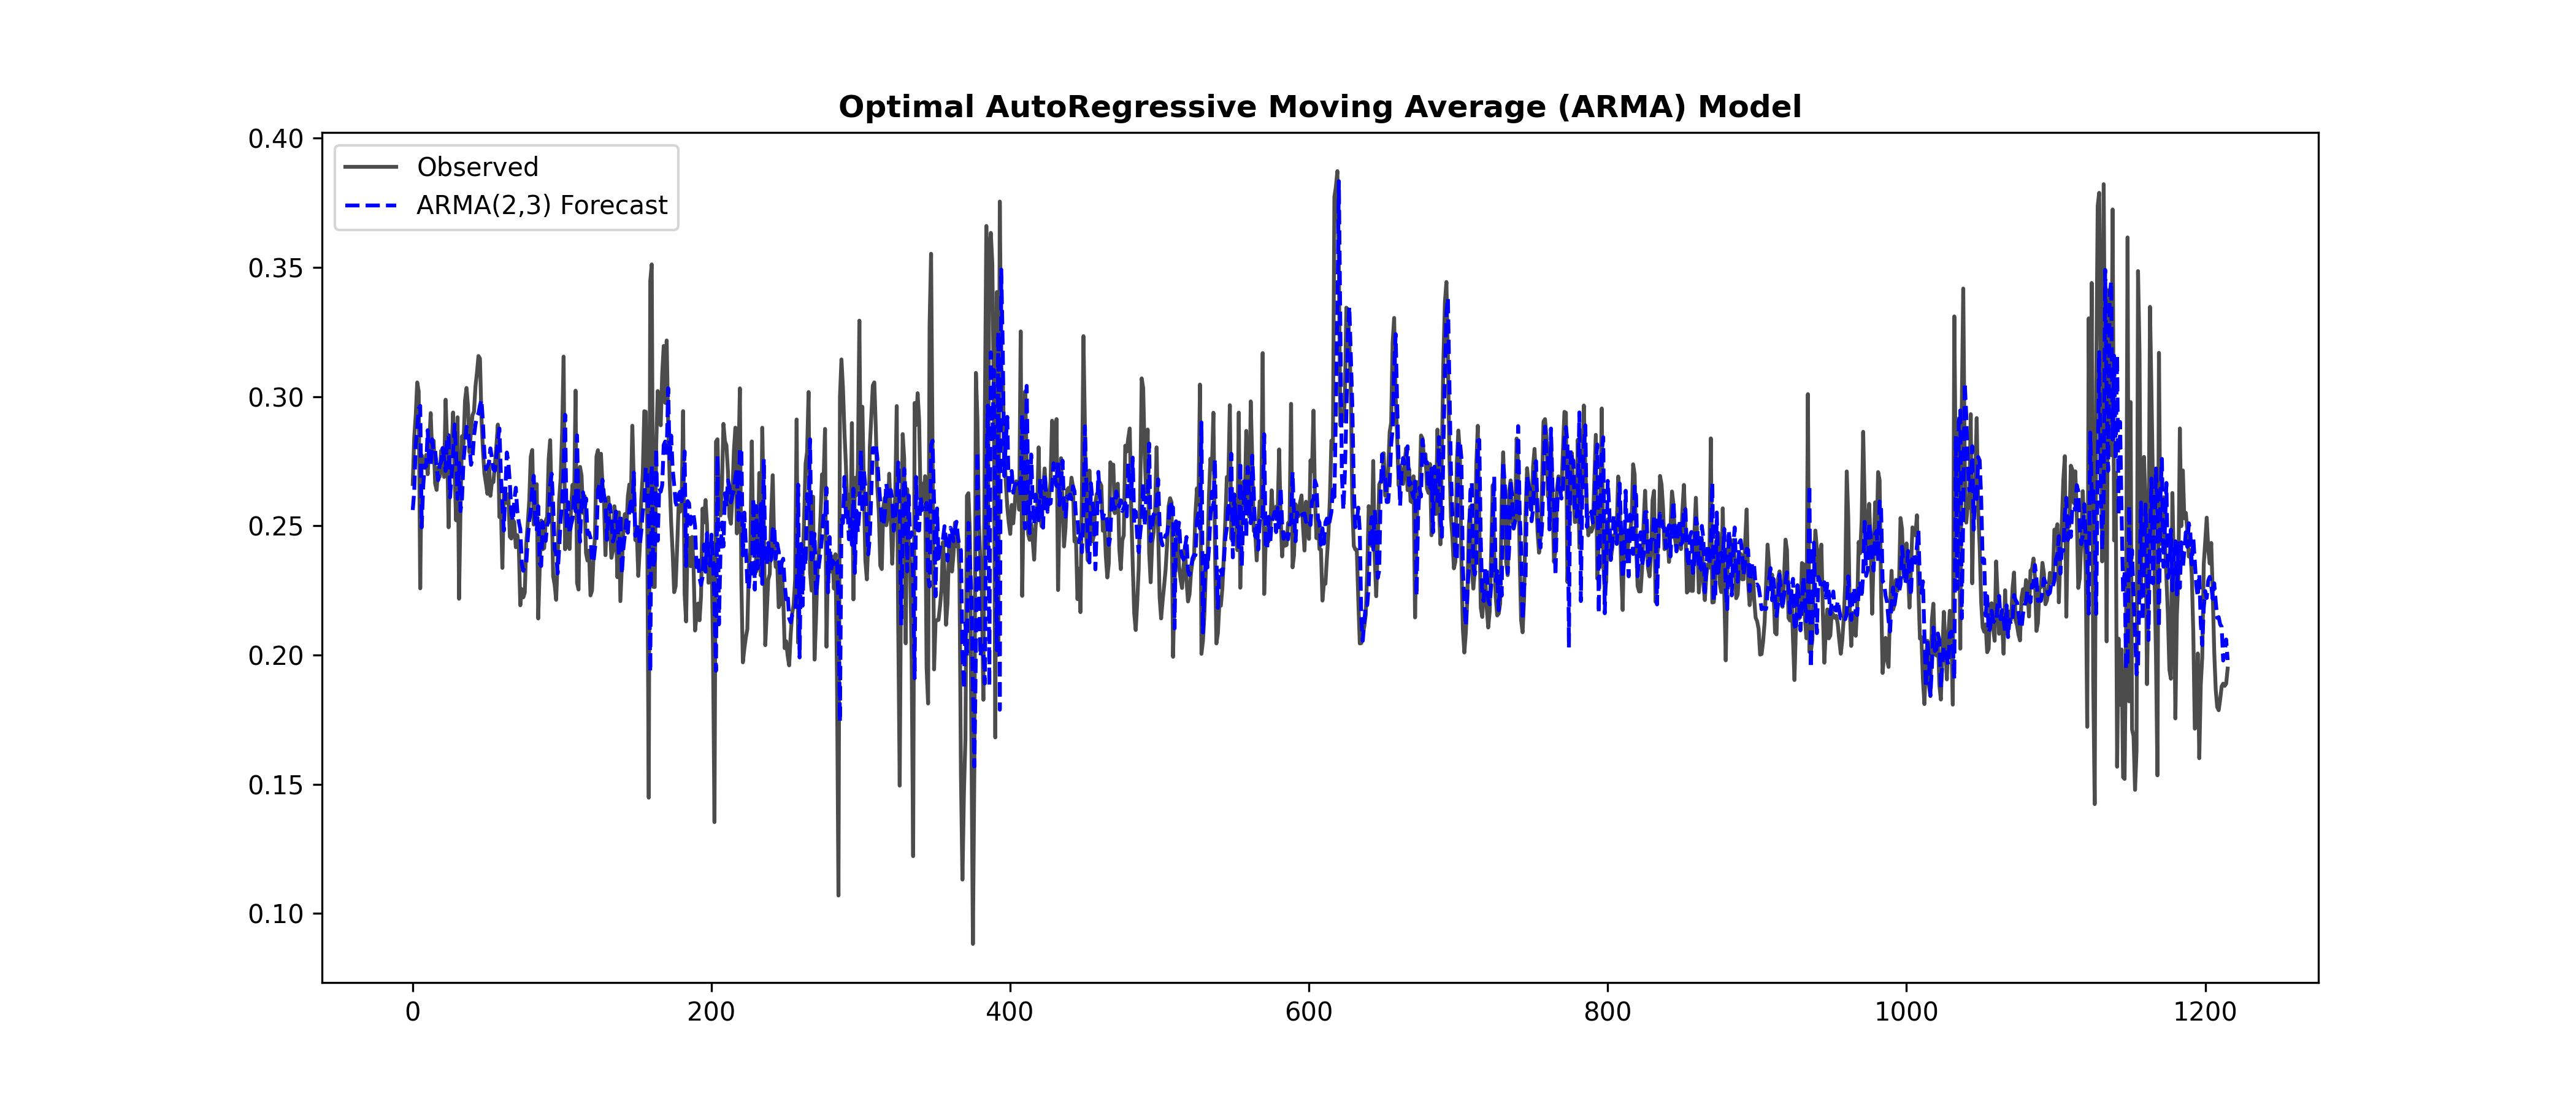
\includegraphics[width=1.0\textwidth]{Forecasting_Graphs/05_ARMA_Optimized.png}
    \end{column}
    \begin{column}{0.3\textwidth}
        \textbf{Theory:}\\
        Optimized hybrid of AR and MA. The theoretical limit of linear univariate models.\\[0.4cm]
        \slidemetrics{ARMA(2,3)}{0.0206}{0.0316}{8.60}{0.2204}
    \end{column}
\end{columns}
\end{frame}

\begin{frame}{Model 6: Seasonal ARIMA (SARIMA)}
\begin{columns}
    \begin{column}{0.65\textwidth}
        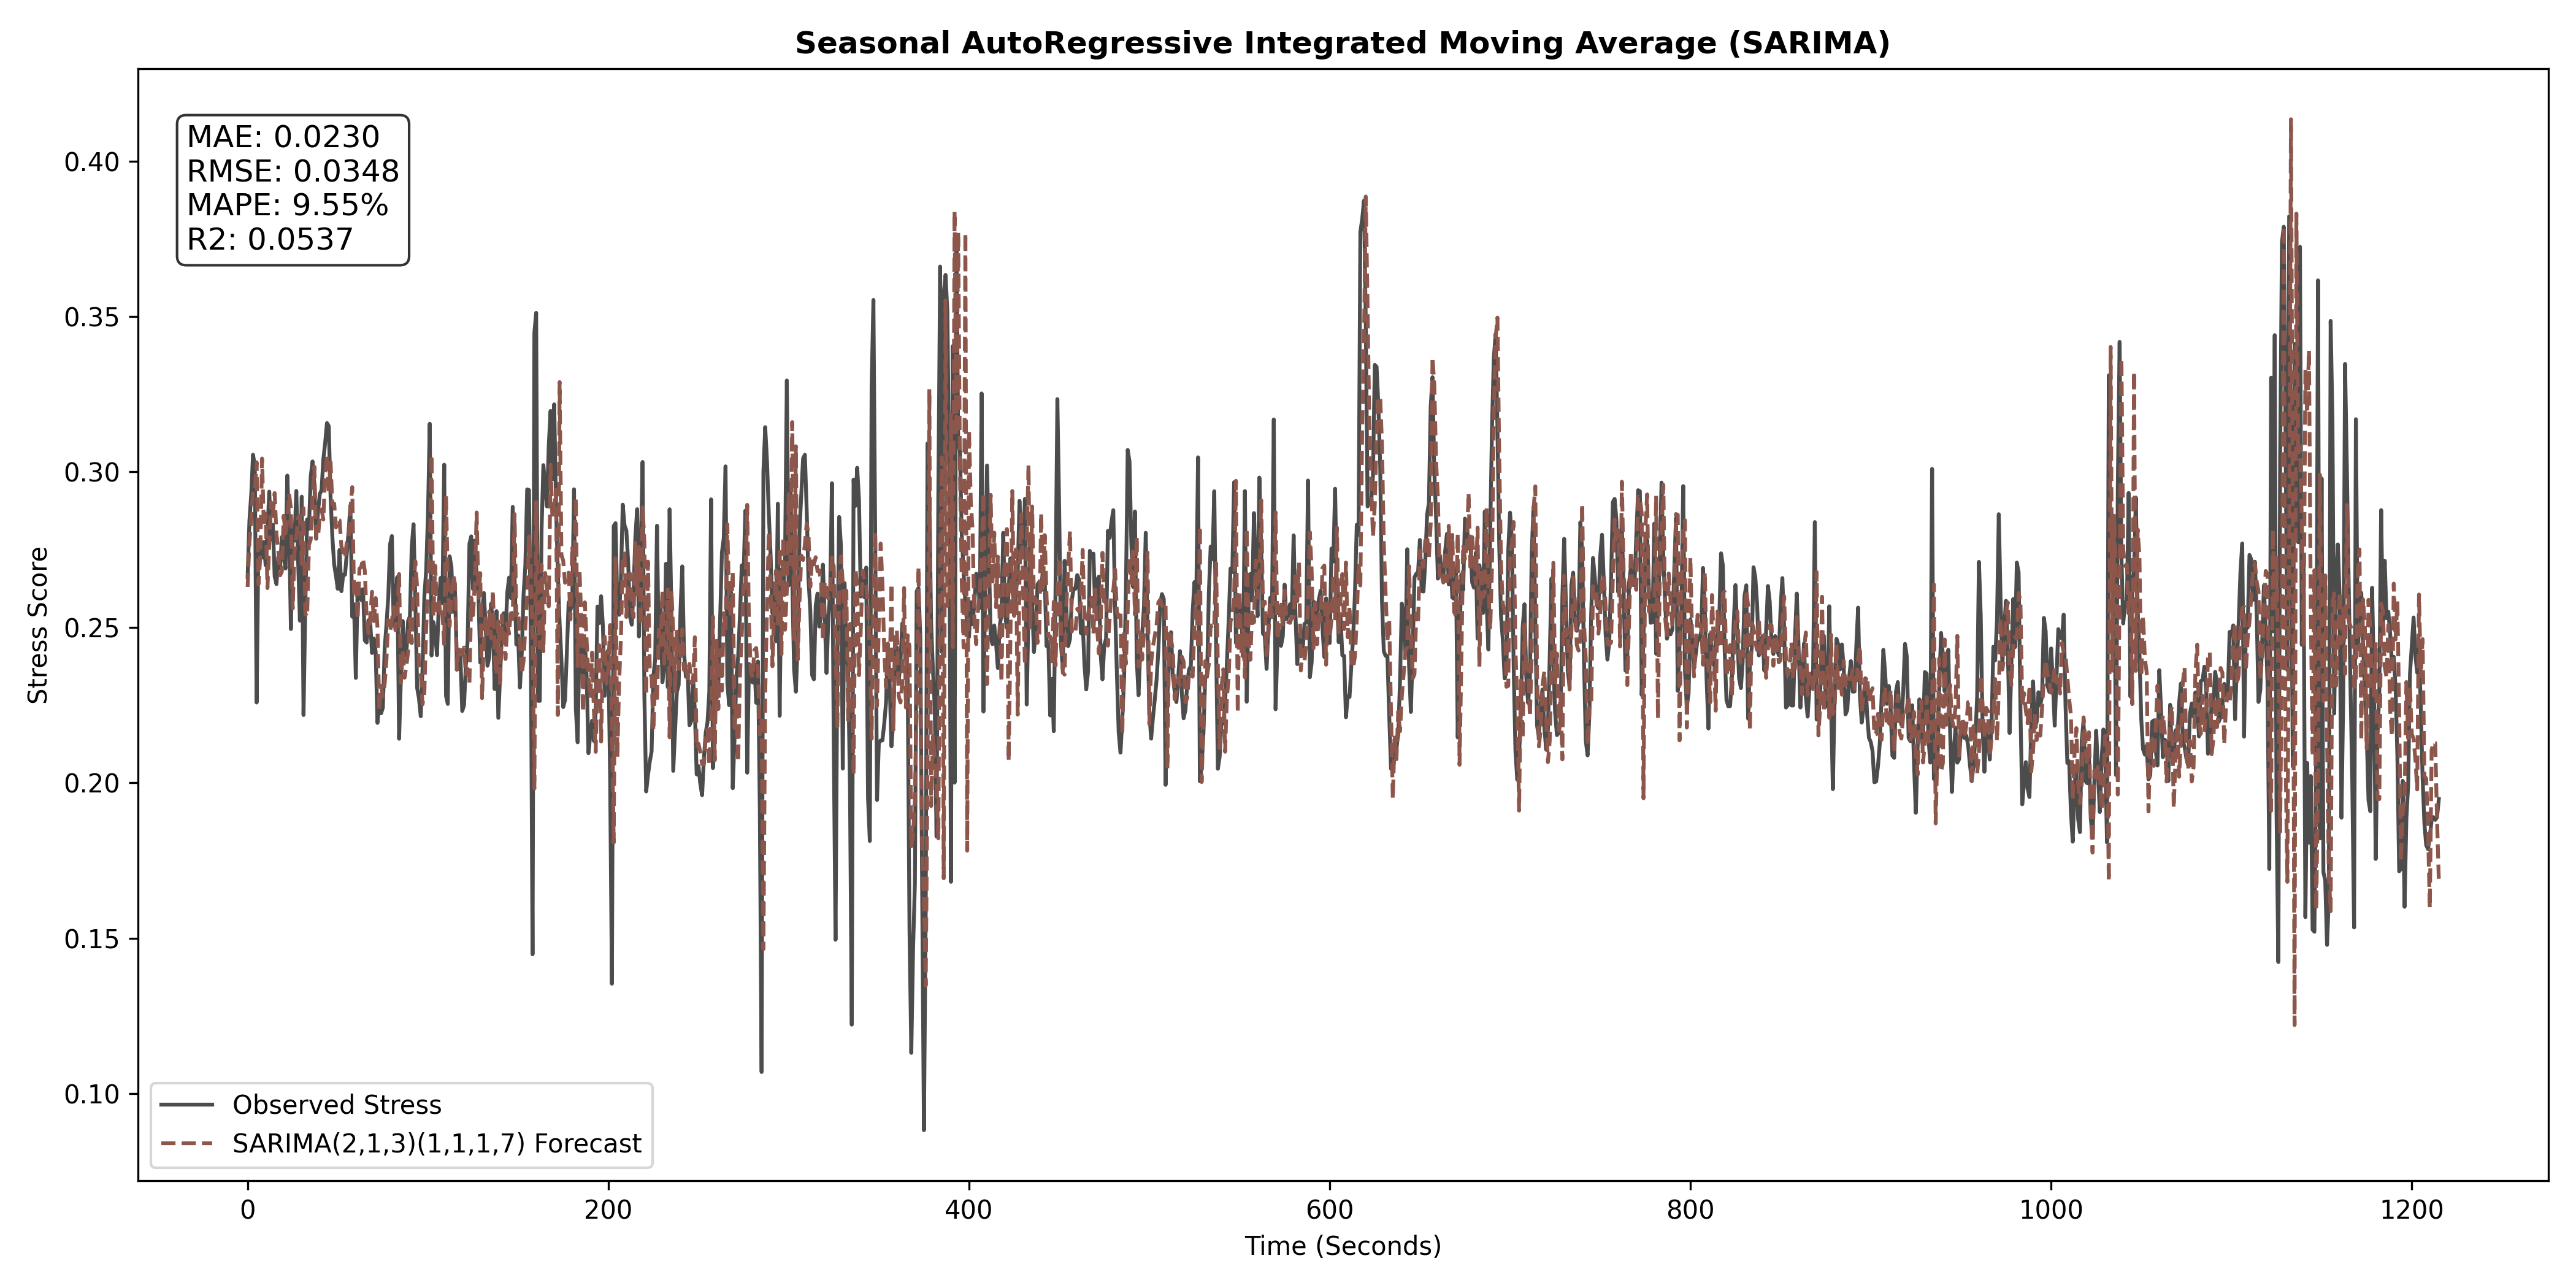
\includegraphics[width=1.0\textwidth]{Forecasting_Graphs/06_SARIMA_Optimized.png}
    \end{column}
    \begin{column}{0.3\textwidth}
        \textbf{Theory:}\\
        Adds $s=7$ to capture high-frequency repeating cycles (e.g., respiration alignment).\\[0.4cm]
        \slidemetrics{SARIMA}{0.0230}{0.0348}{9.55}{0.0537}
    \end{column}
\end{columns}
\end{frame}

\begin{frame}{Model 7: SARIMAX (Exogenous Variables)}
\begin{columns}
    \begin{column}{0.65\textwidth}
        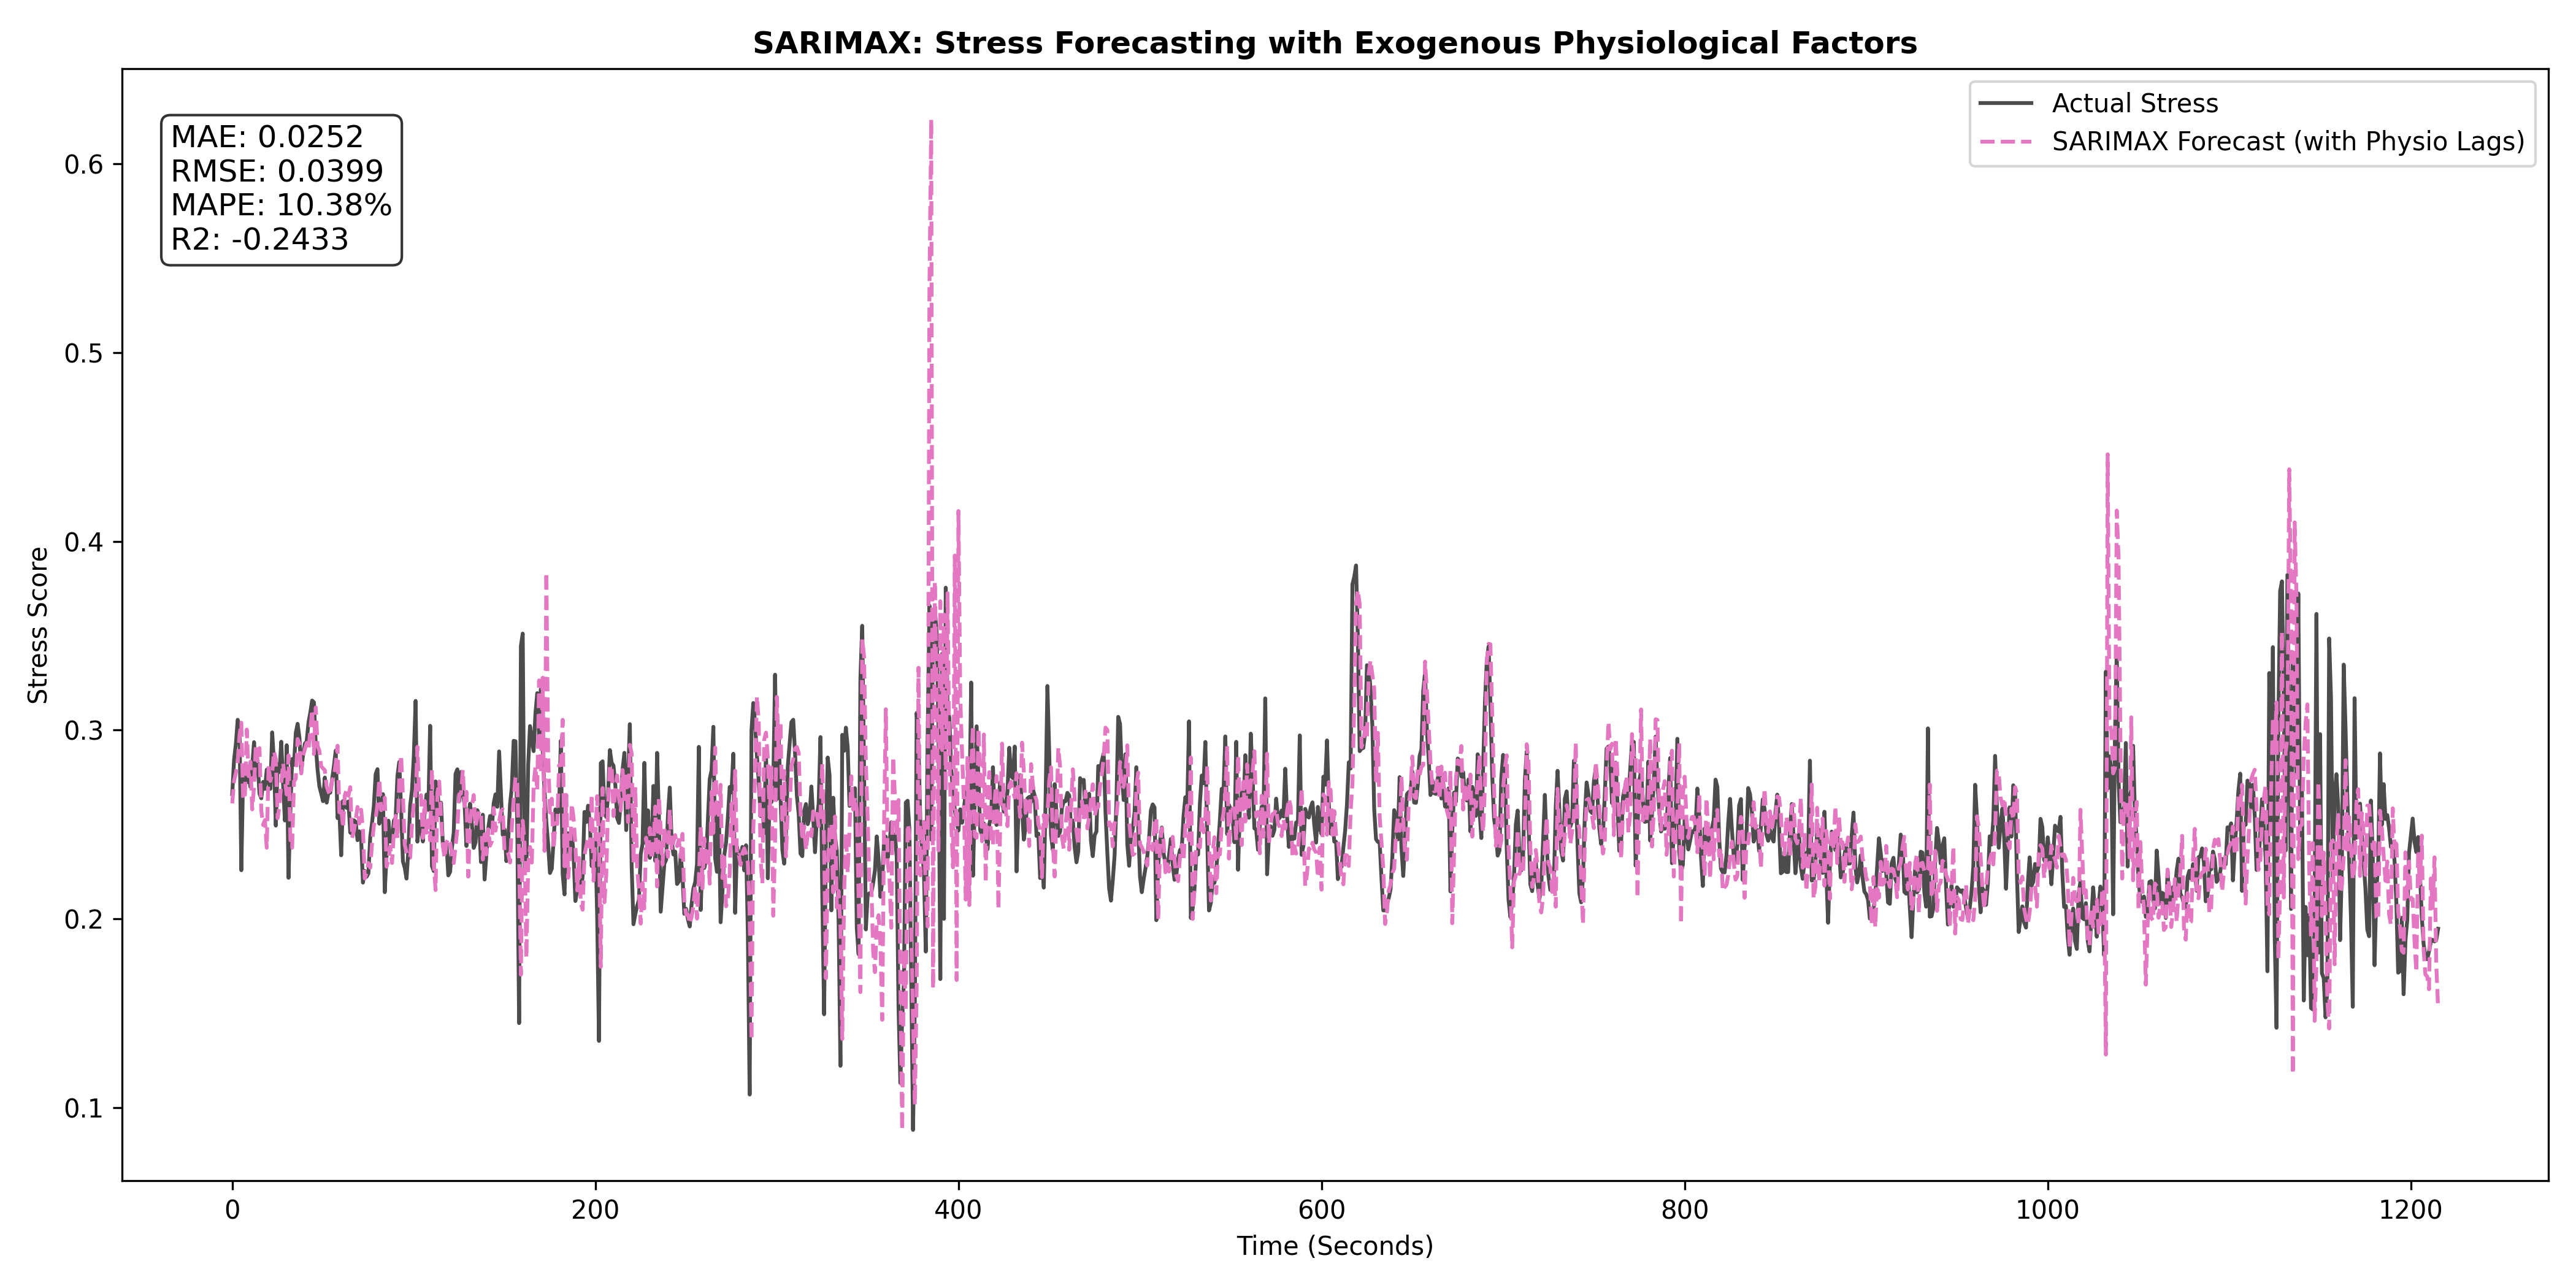
\includegraphics[width=1.0\textwidth]{Forecasting_Graphs/07_SARIMAX_Optimized.png}
    \end{column}
    \begin{column}{0.3\textwidth}
        \textbf{Theory:}\\
        Incorporates $t-1$ lagged EDA, HR, and TEMP directly into the statistical equation.\\[0.4cm]
        \slidemetrics{SARIMAX}{0.0252}{0.0399}{10.38}{-0.2433}
    \end{column}
\end{columns}
\end{frame}

\begin{frame}{Model 8: Random Forest Regressor}
\begin{columns}
    \begin{column}{0.65\textwidth}
        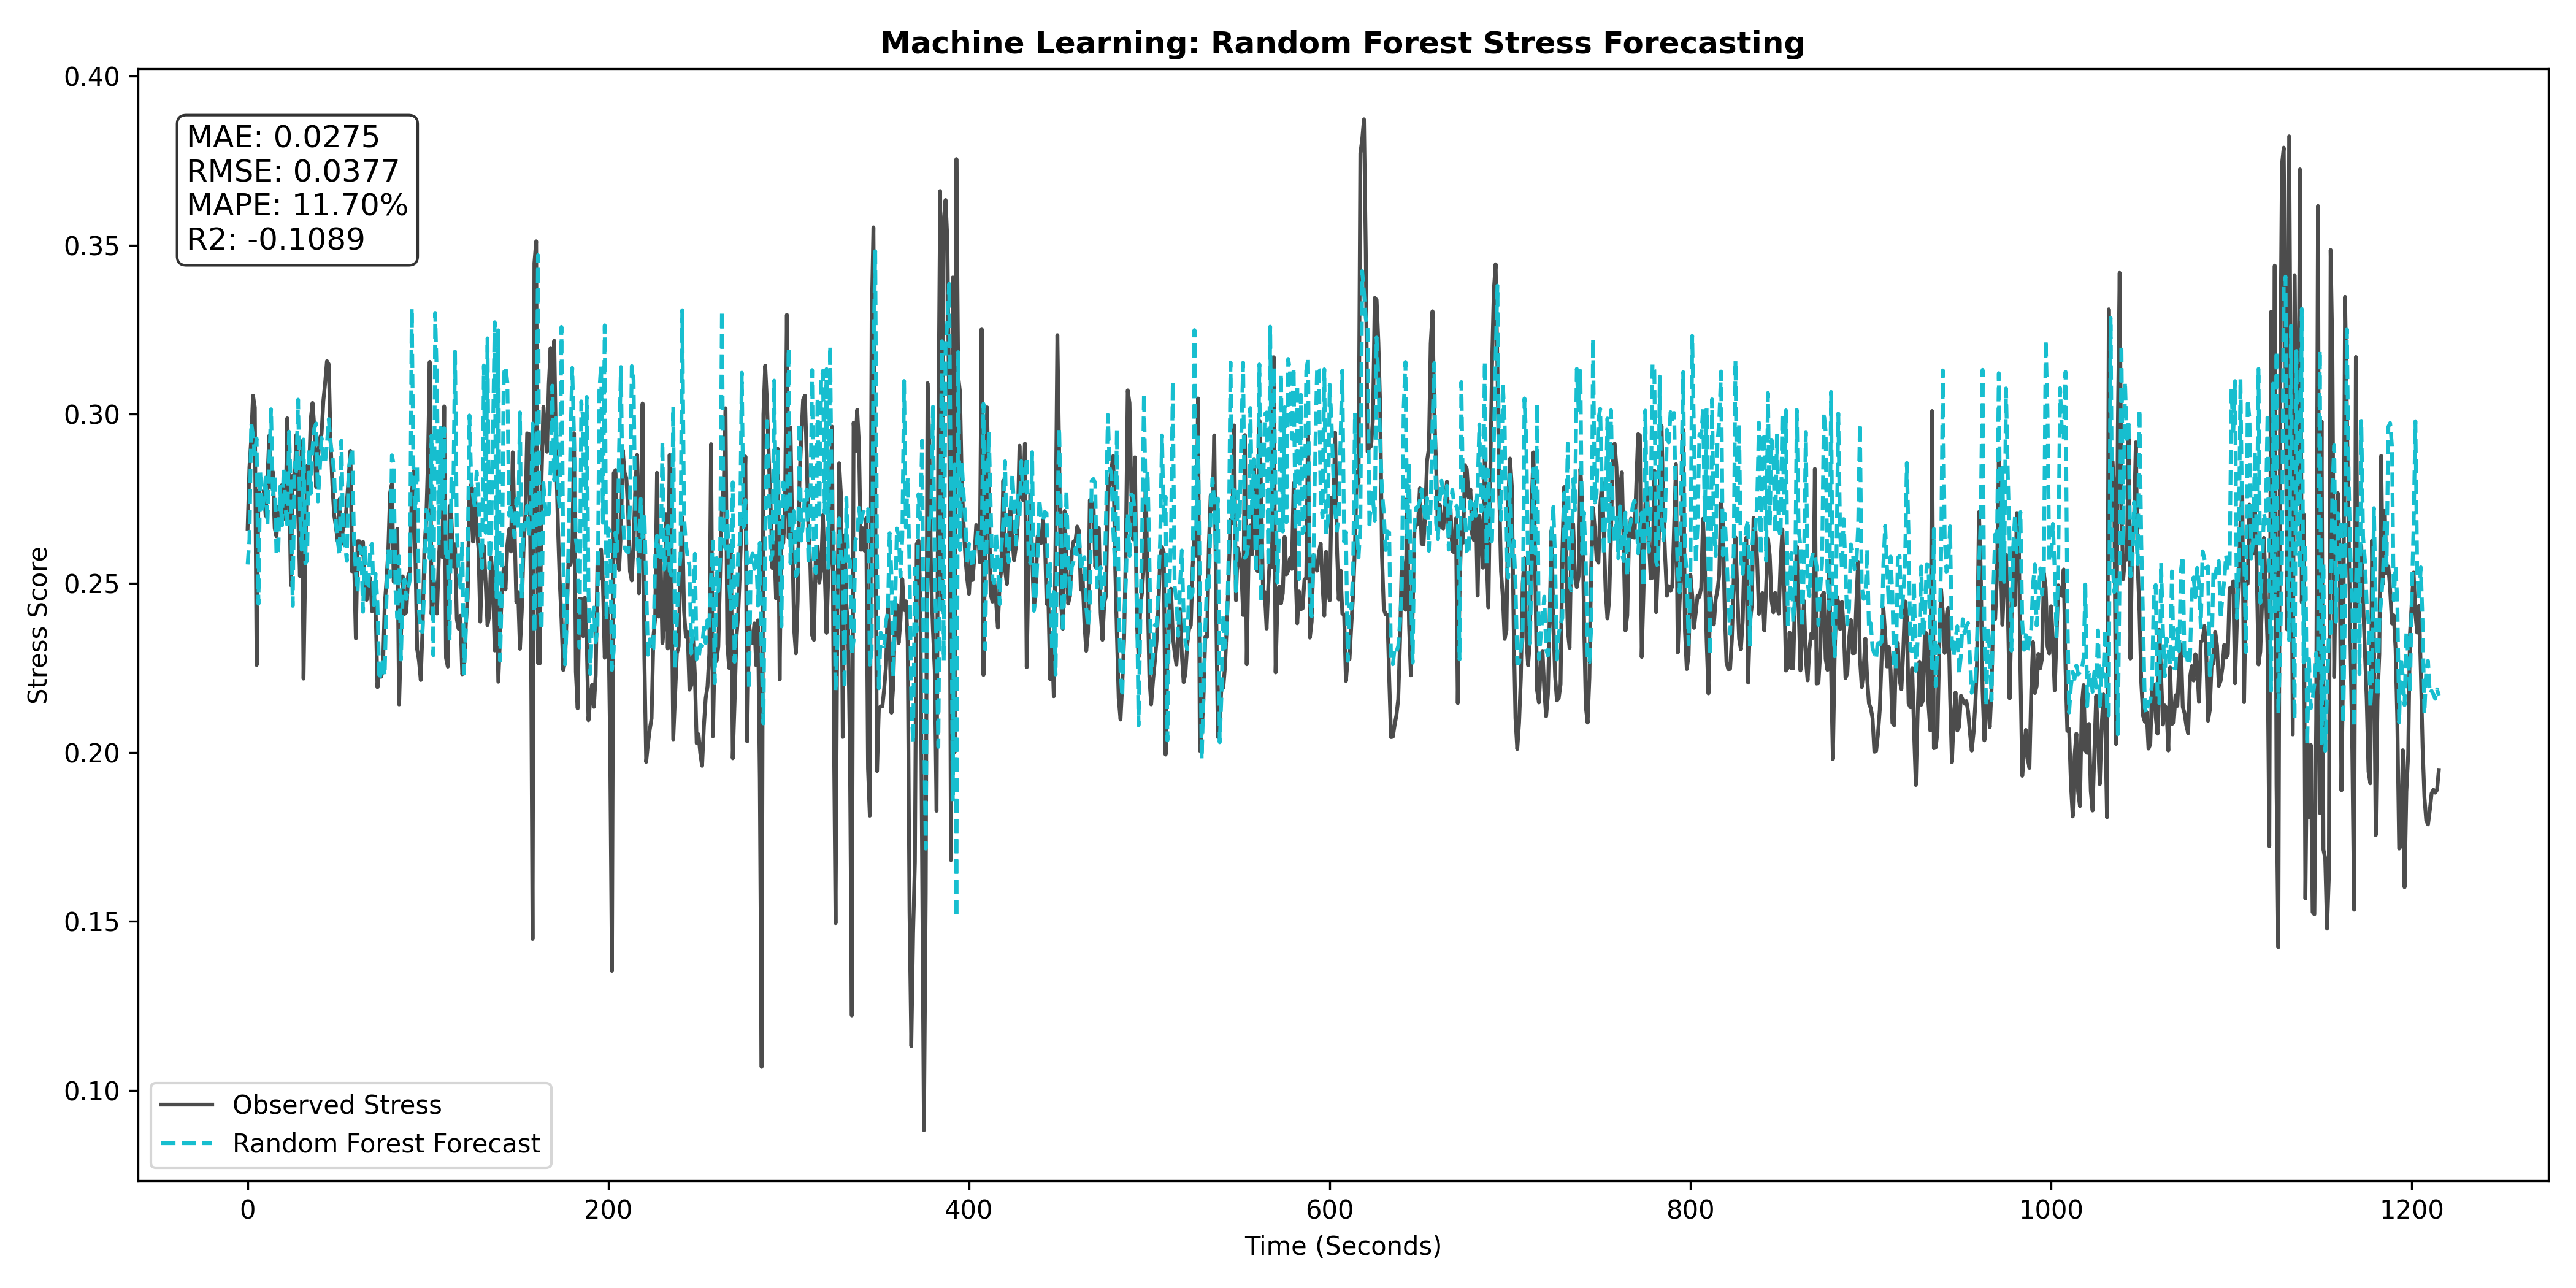
\includegraphics[width=1.0\textwidth]{Forecasting_Graphs/08_Random_Forest_Forecast.png}
    \end{column}
    \begin{column}{0.3\textwidth}
        \textbf{Theory:}\\
        Non-parametric ML. Averages multiple decision trees to handle raw sensor variance.\\[0.4cm]
        \slidemetrics{Random Forest}{0.0275}{0.0377}{11.70}{-0.1089}
    \end{column}
\end{columns}
\end{frame}

\begin{frame}{Model 9: XGBoost Regressor}
\begin{columns}
    \begin{column}{0.65\textwidth}
        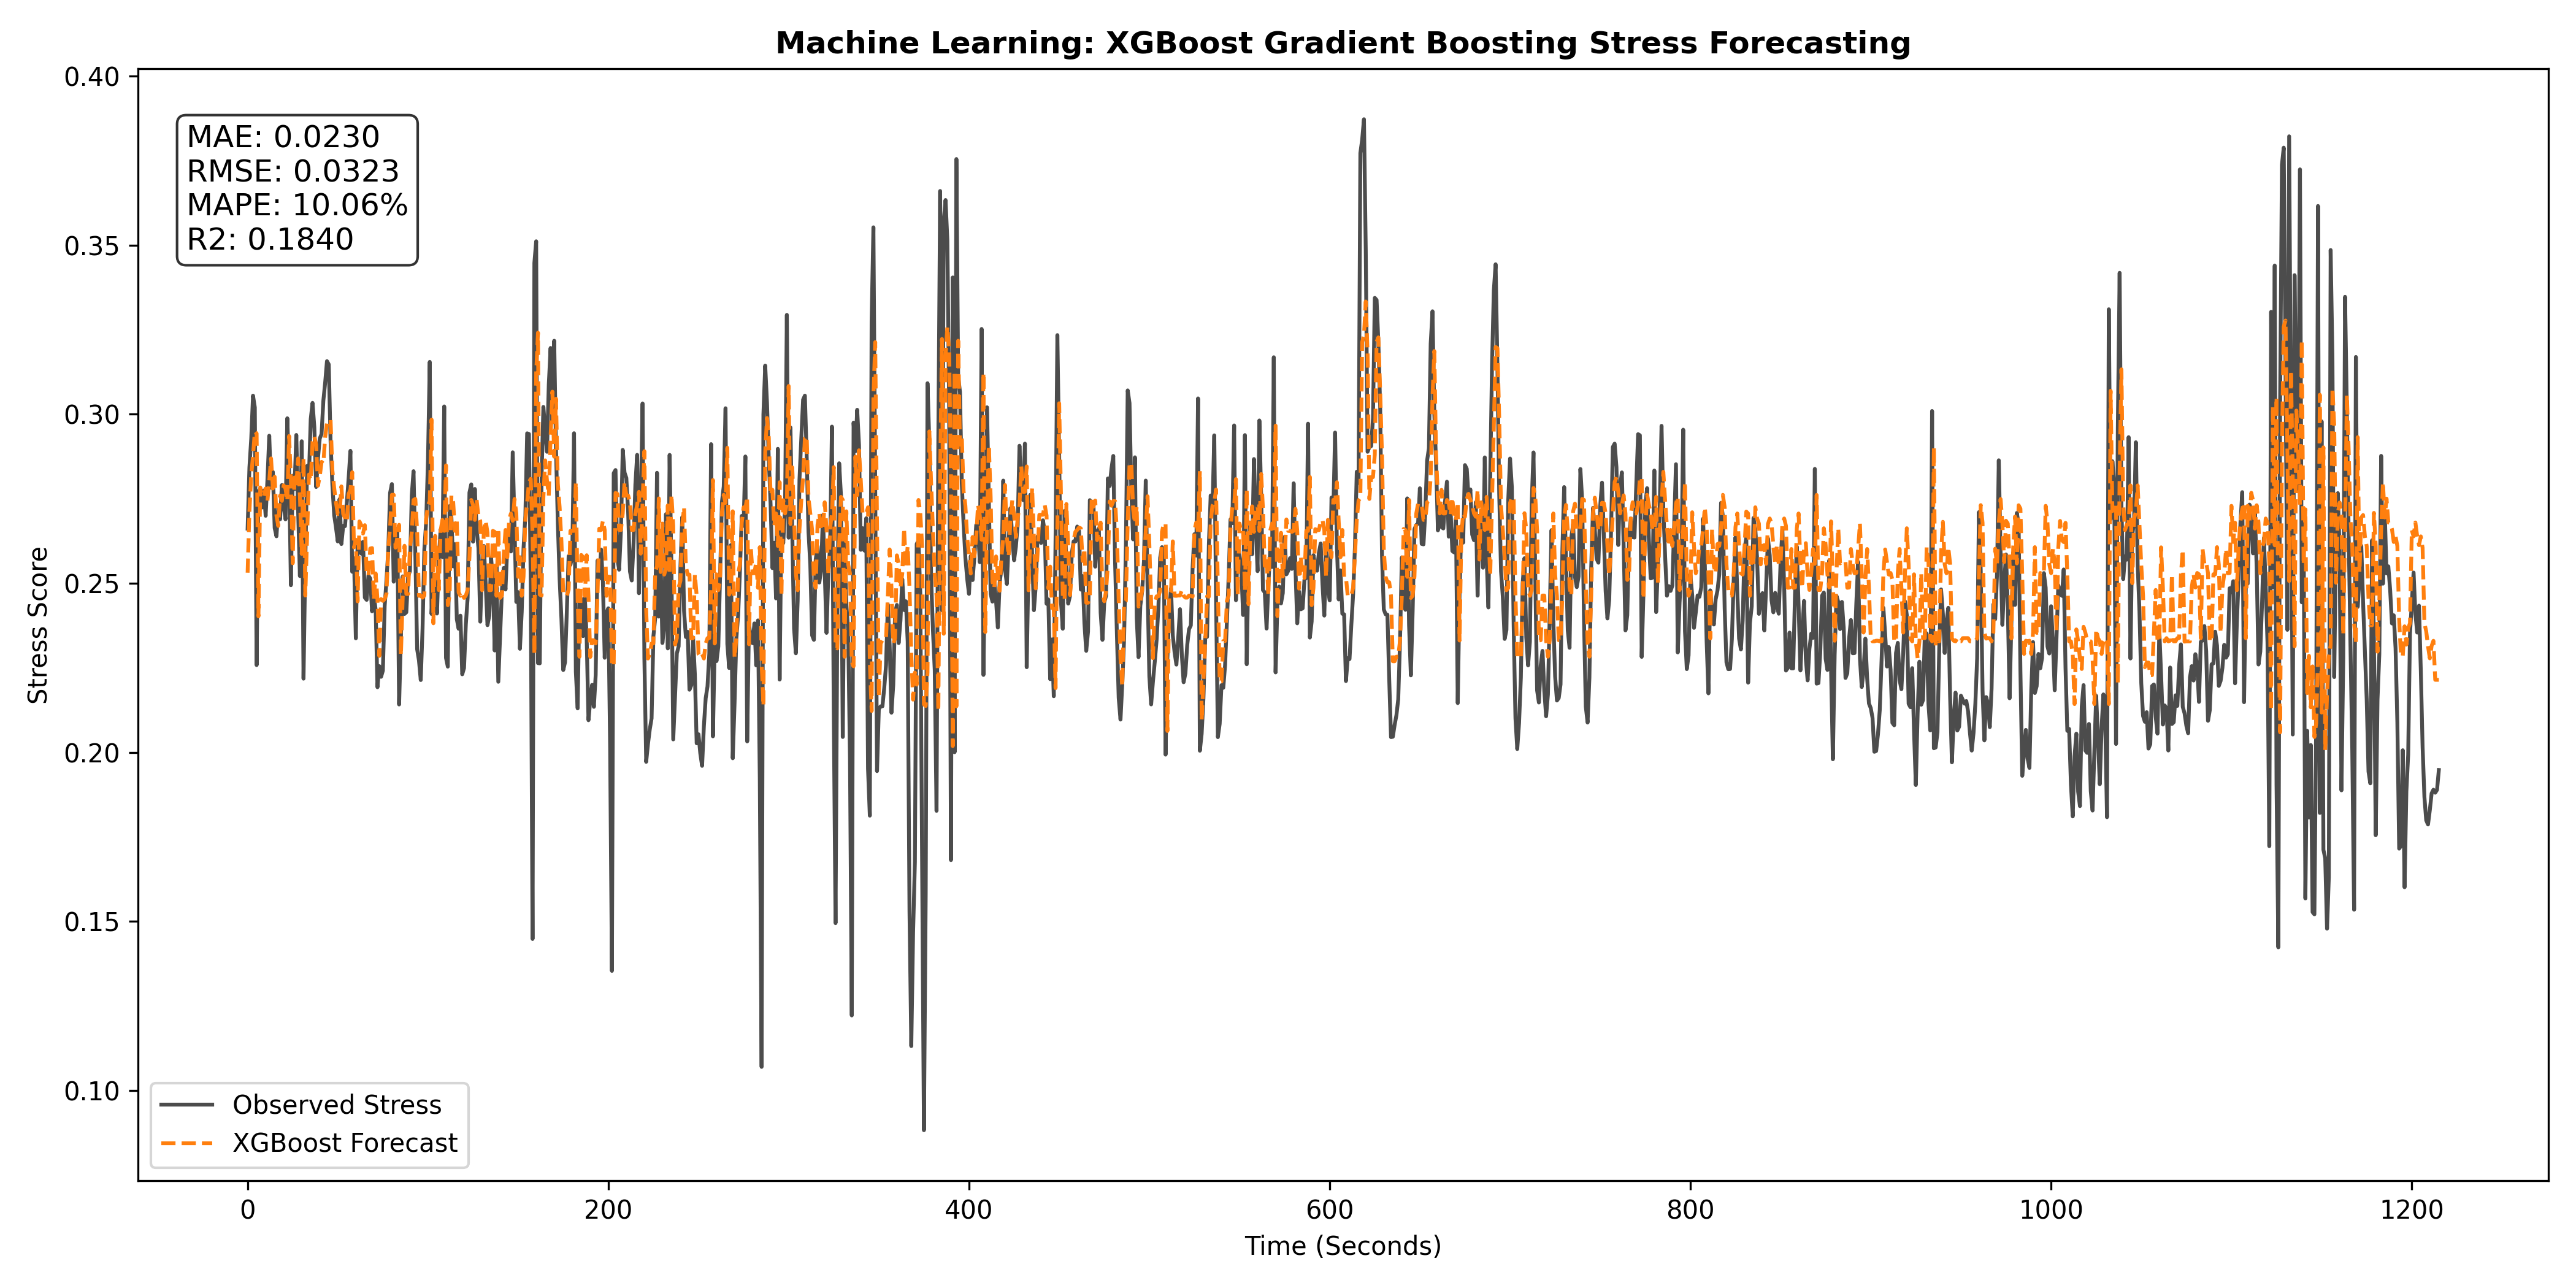
\includegraphics[width=1.0\textwidth]{Forecasting_Graphs/09_XGBoost_Forecast.png}
    \end{column}
    \begin{column}{0.3\textwidth}
        \textbf{Theory:}\\
        Iterative Gradient Boosting. Finds complex non-linear thresholds in physiological data.\\[0.4cm]
        \slidemetrics{XGBoost}{0.0230}{0.0323}{10.06}{0.1840}
    \end{column}
\end{columns}
\end{frame}

\begin{frame}{Model 10: LSTM (Deep Learning Leader)}
\begin{columns}
    \begin{column}{0.65\textwidth}
        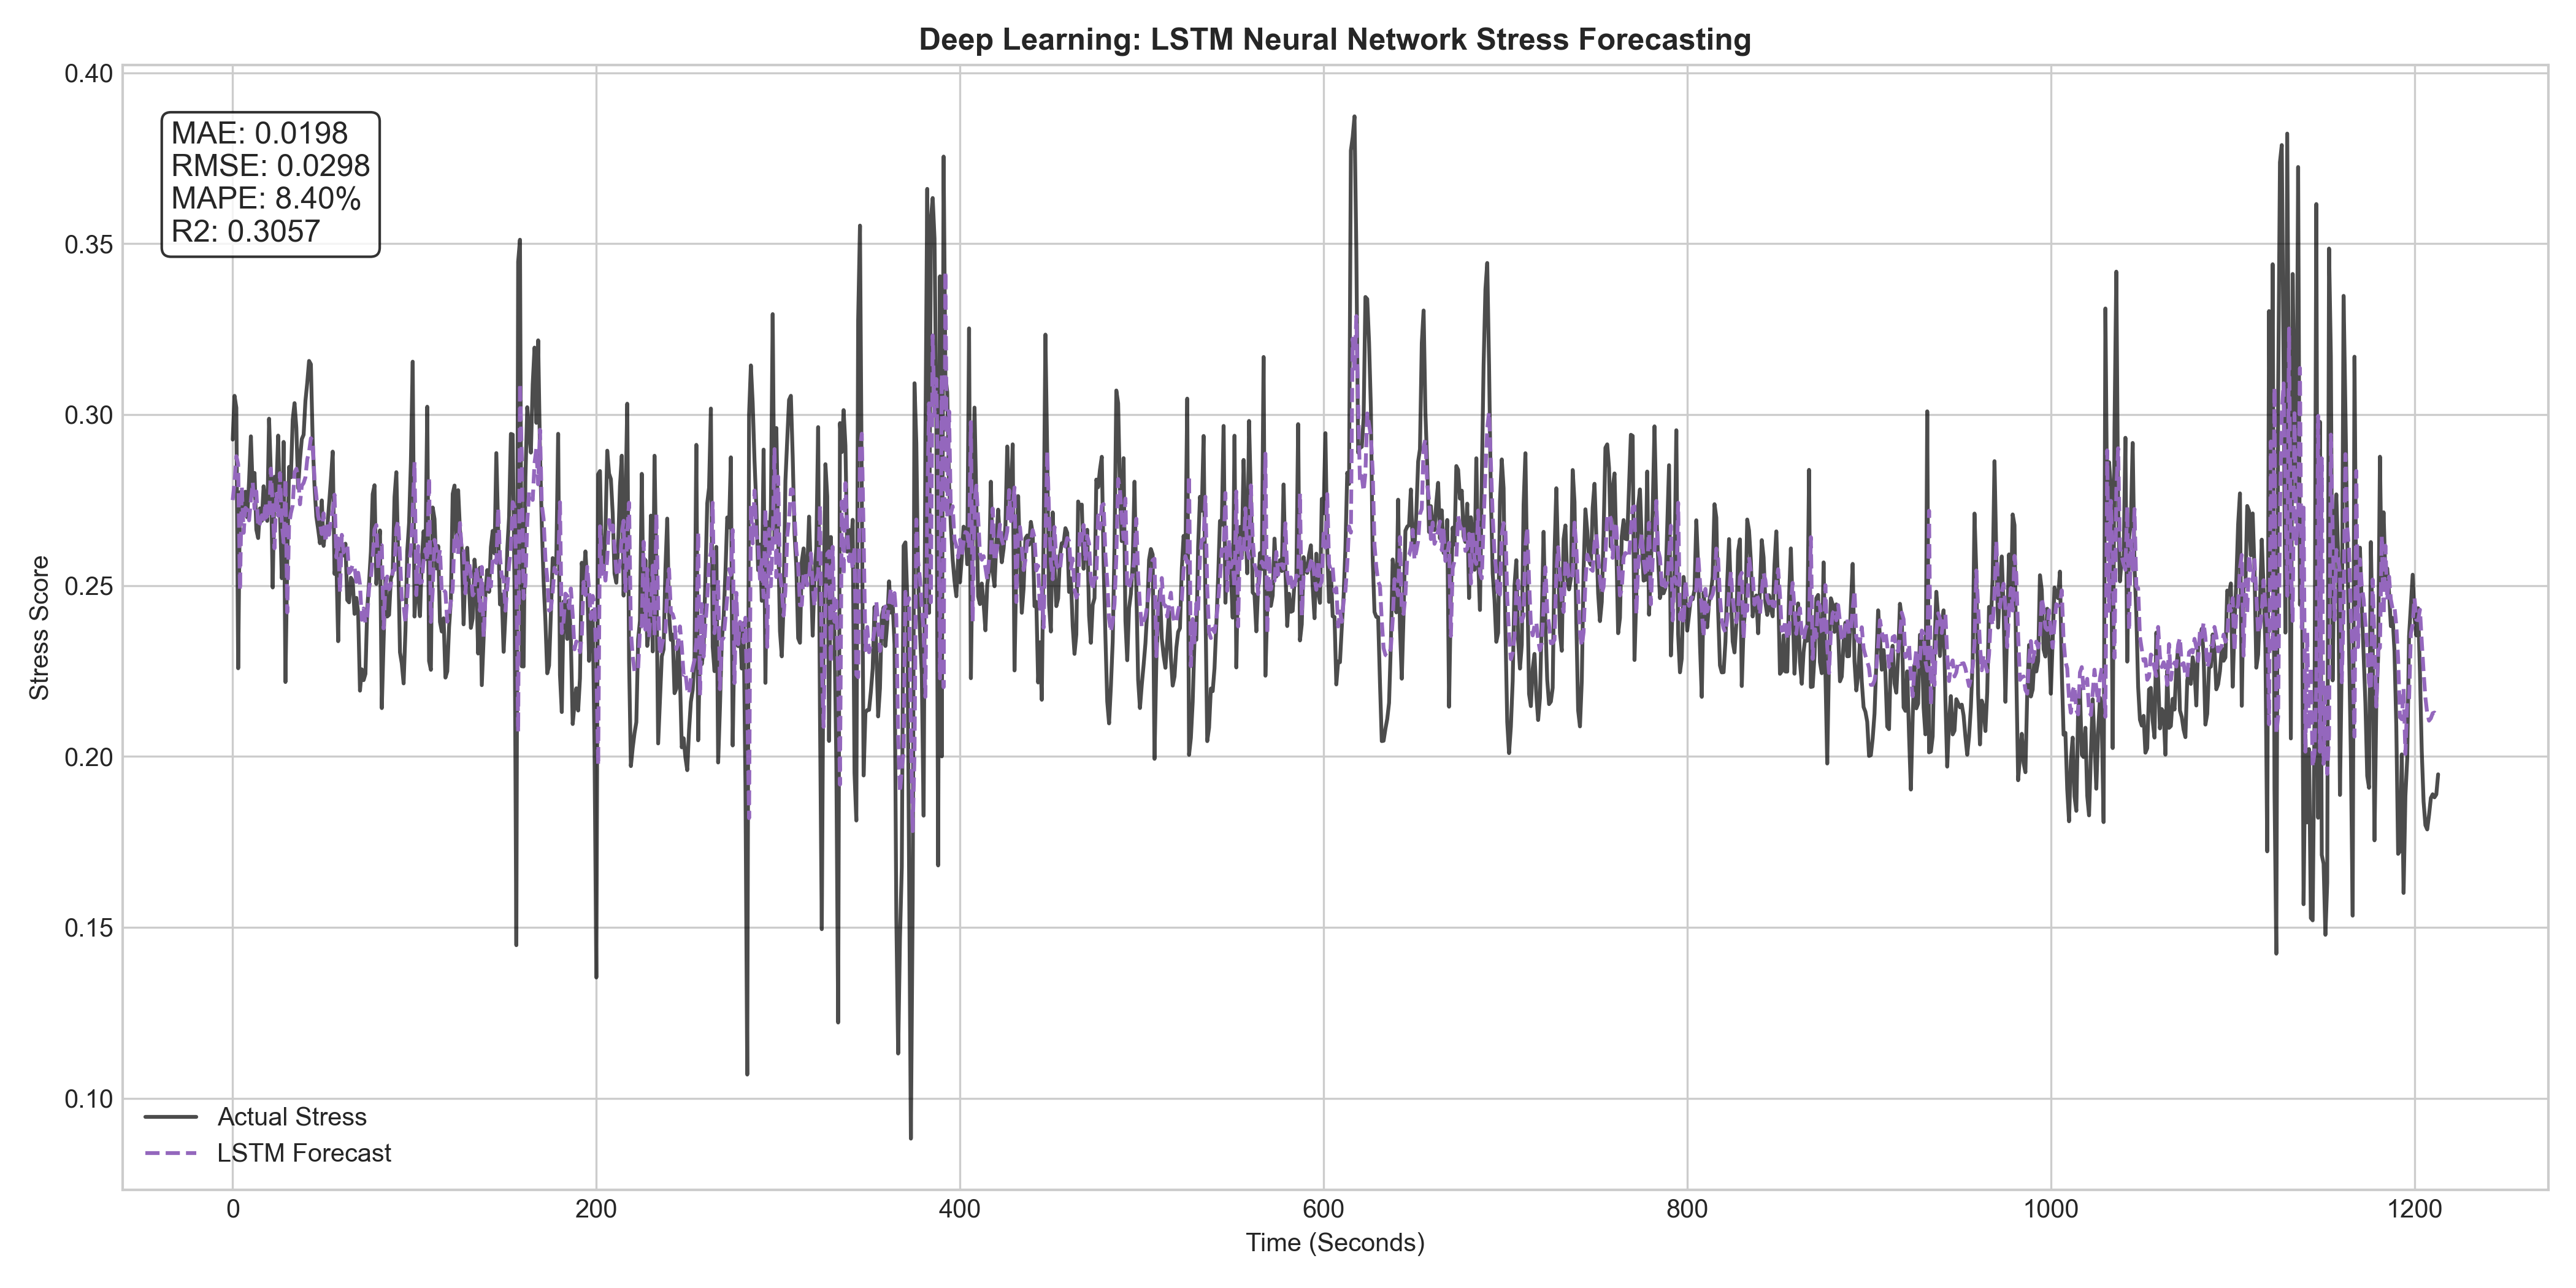
\includegraphics[width=1.0\textwidth]{Forecasting_Graphs/10_LSTM_Forecast.png}
    \end{column}
    \begin{column}{0.3\textwidth}
        \textbf{Theory:}\\
        Recurrent memory cells bypass the vanishing gradient, capturing 10-second temporal sequences.\\[0.4cm]
        \slidemetrics{LSTM}{0.0198}{0.0298}{8.40}{0.3057}
    \end{column}
\end{columns}
\end{frame}

\begin{frame}{Model 11: Support Vector Regression (SVR)}
\begin{columns}
    \begin{column}{0.65\textwidth}
        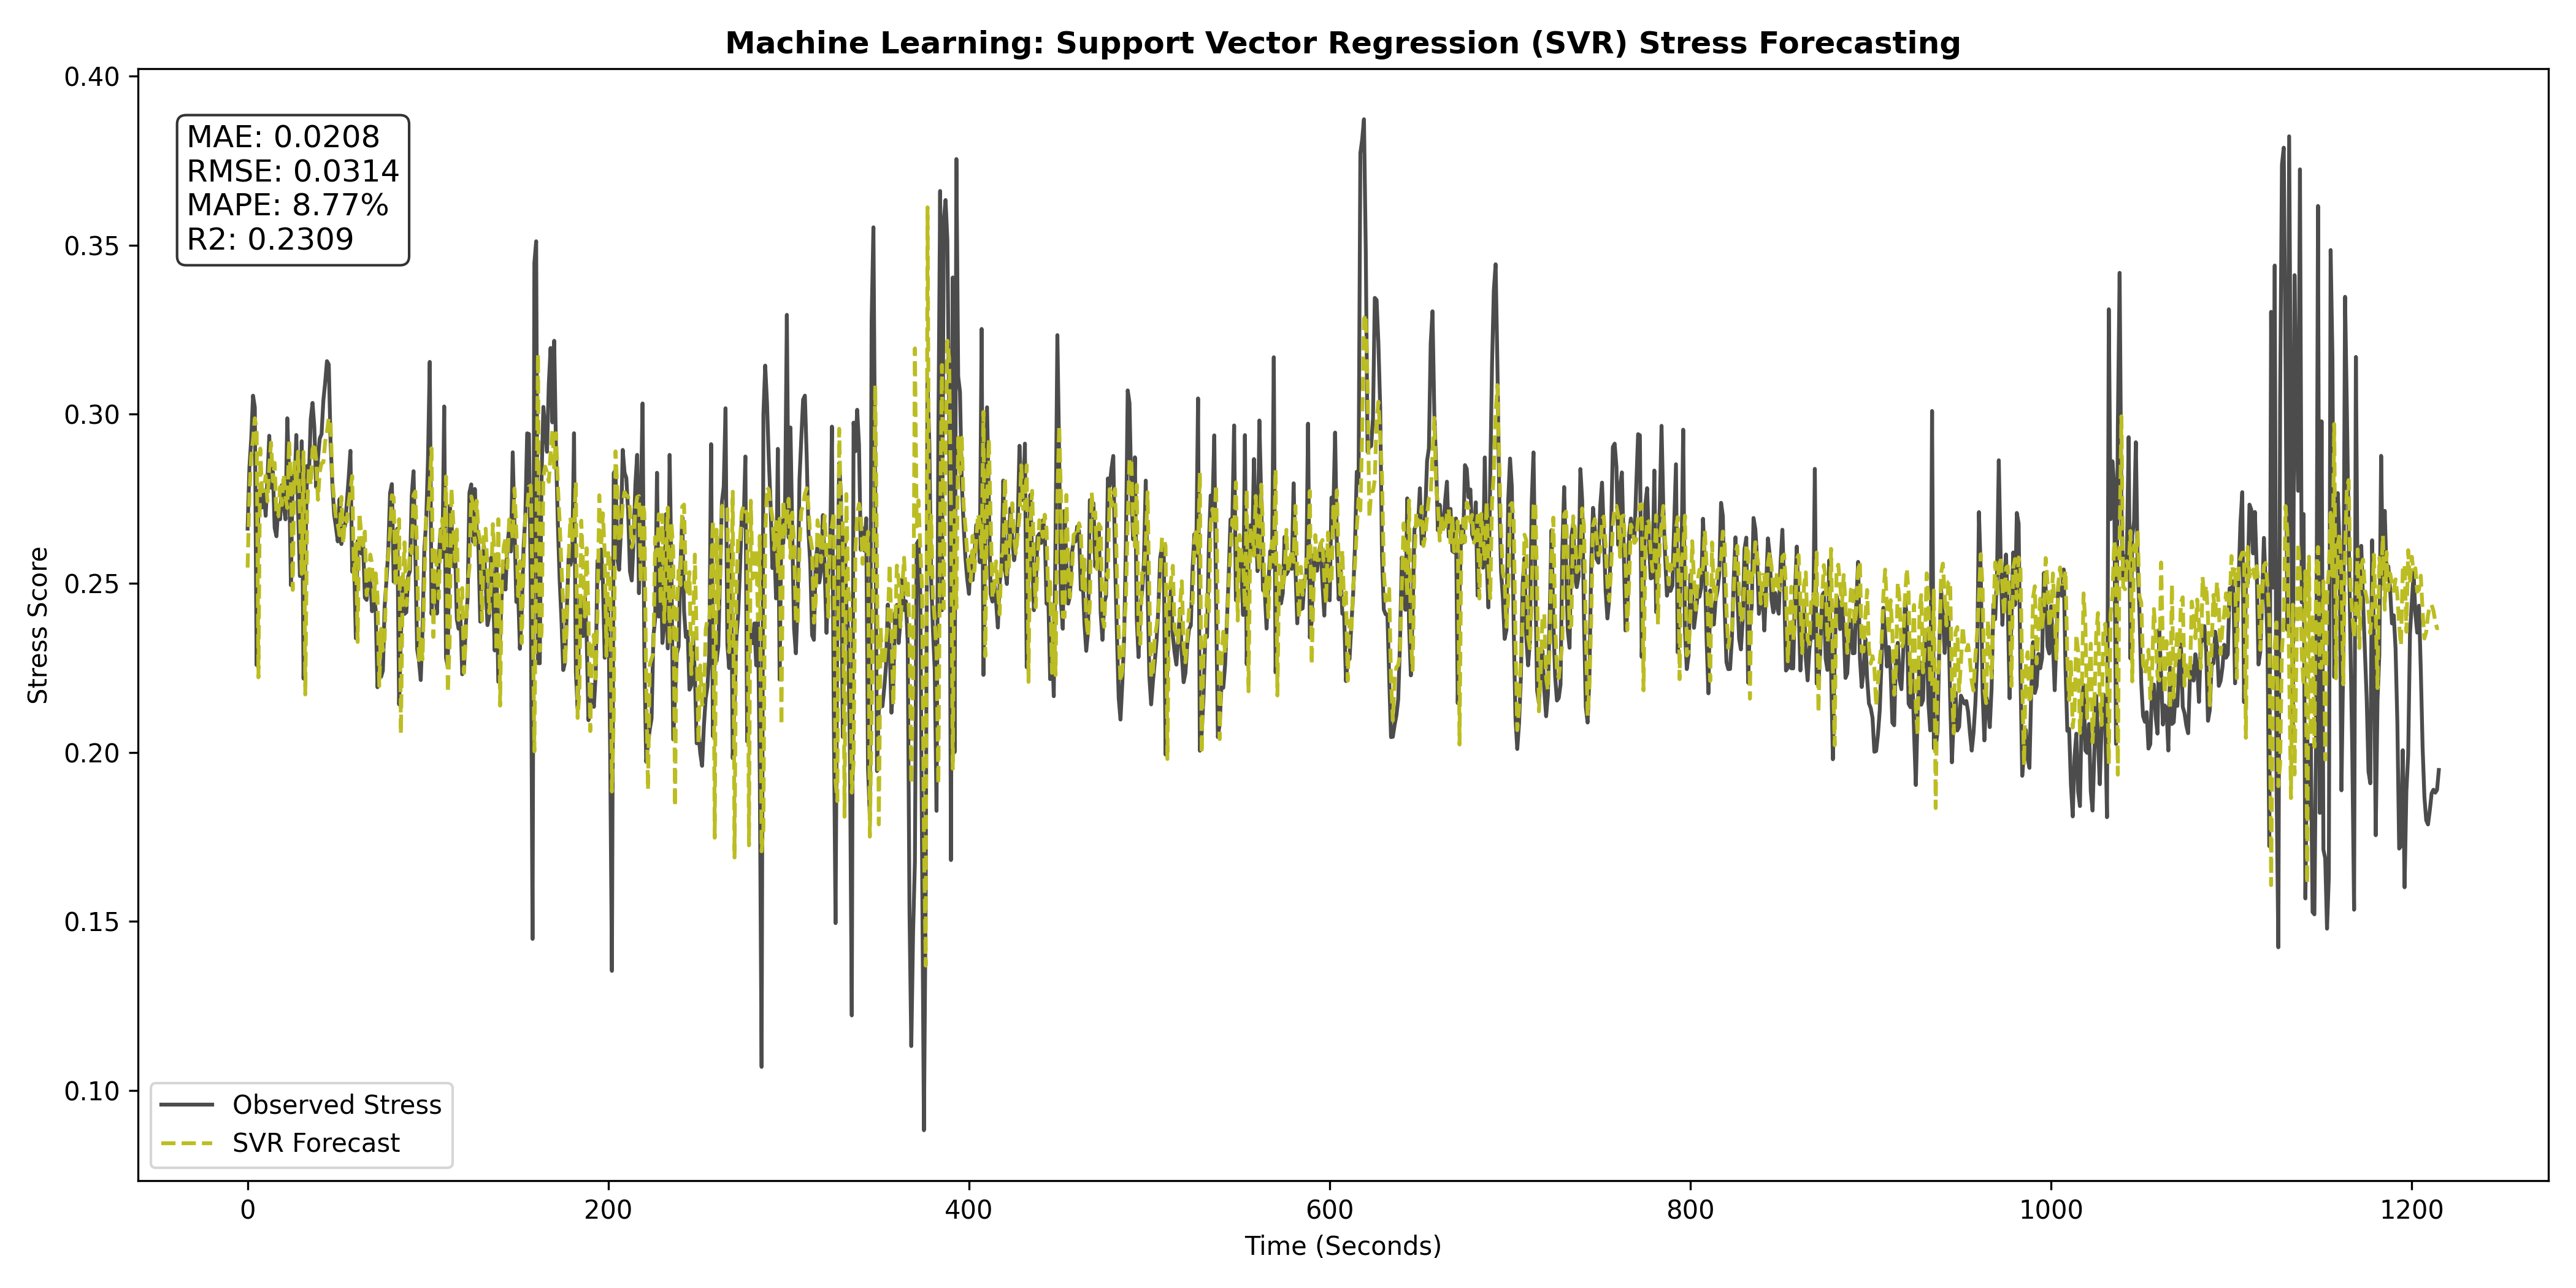
\includegraphics[width=1.0\textwidth]{Forecasting_Graphs/11_SVR_Forecast.png}
    \end{column}
    \begin{column}{0.3\textwidth}
        \textbf{Theory:}\\
        Uses RBF kernels to project inputs into higher dimensions, finding clean margins.\\[0.4cm]
        \slidemetrics{SVR}{0.0208}{0.0314}{8.77}{0.2309}
    \end{column}
\end{columns}
\end{frame}

\begin{frame}{Model 12: GRU Neural Network}
\begin{columns}
    \begin{column}{0.65\textwidth}
        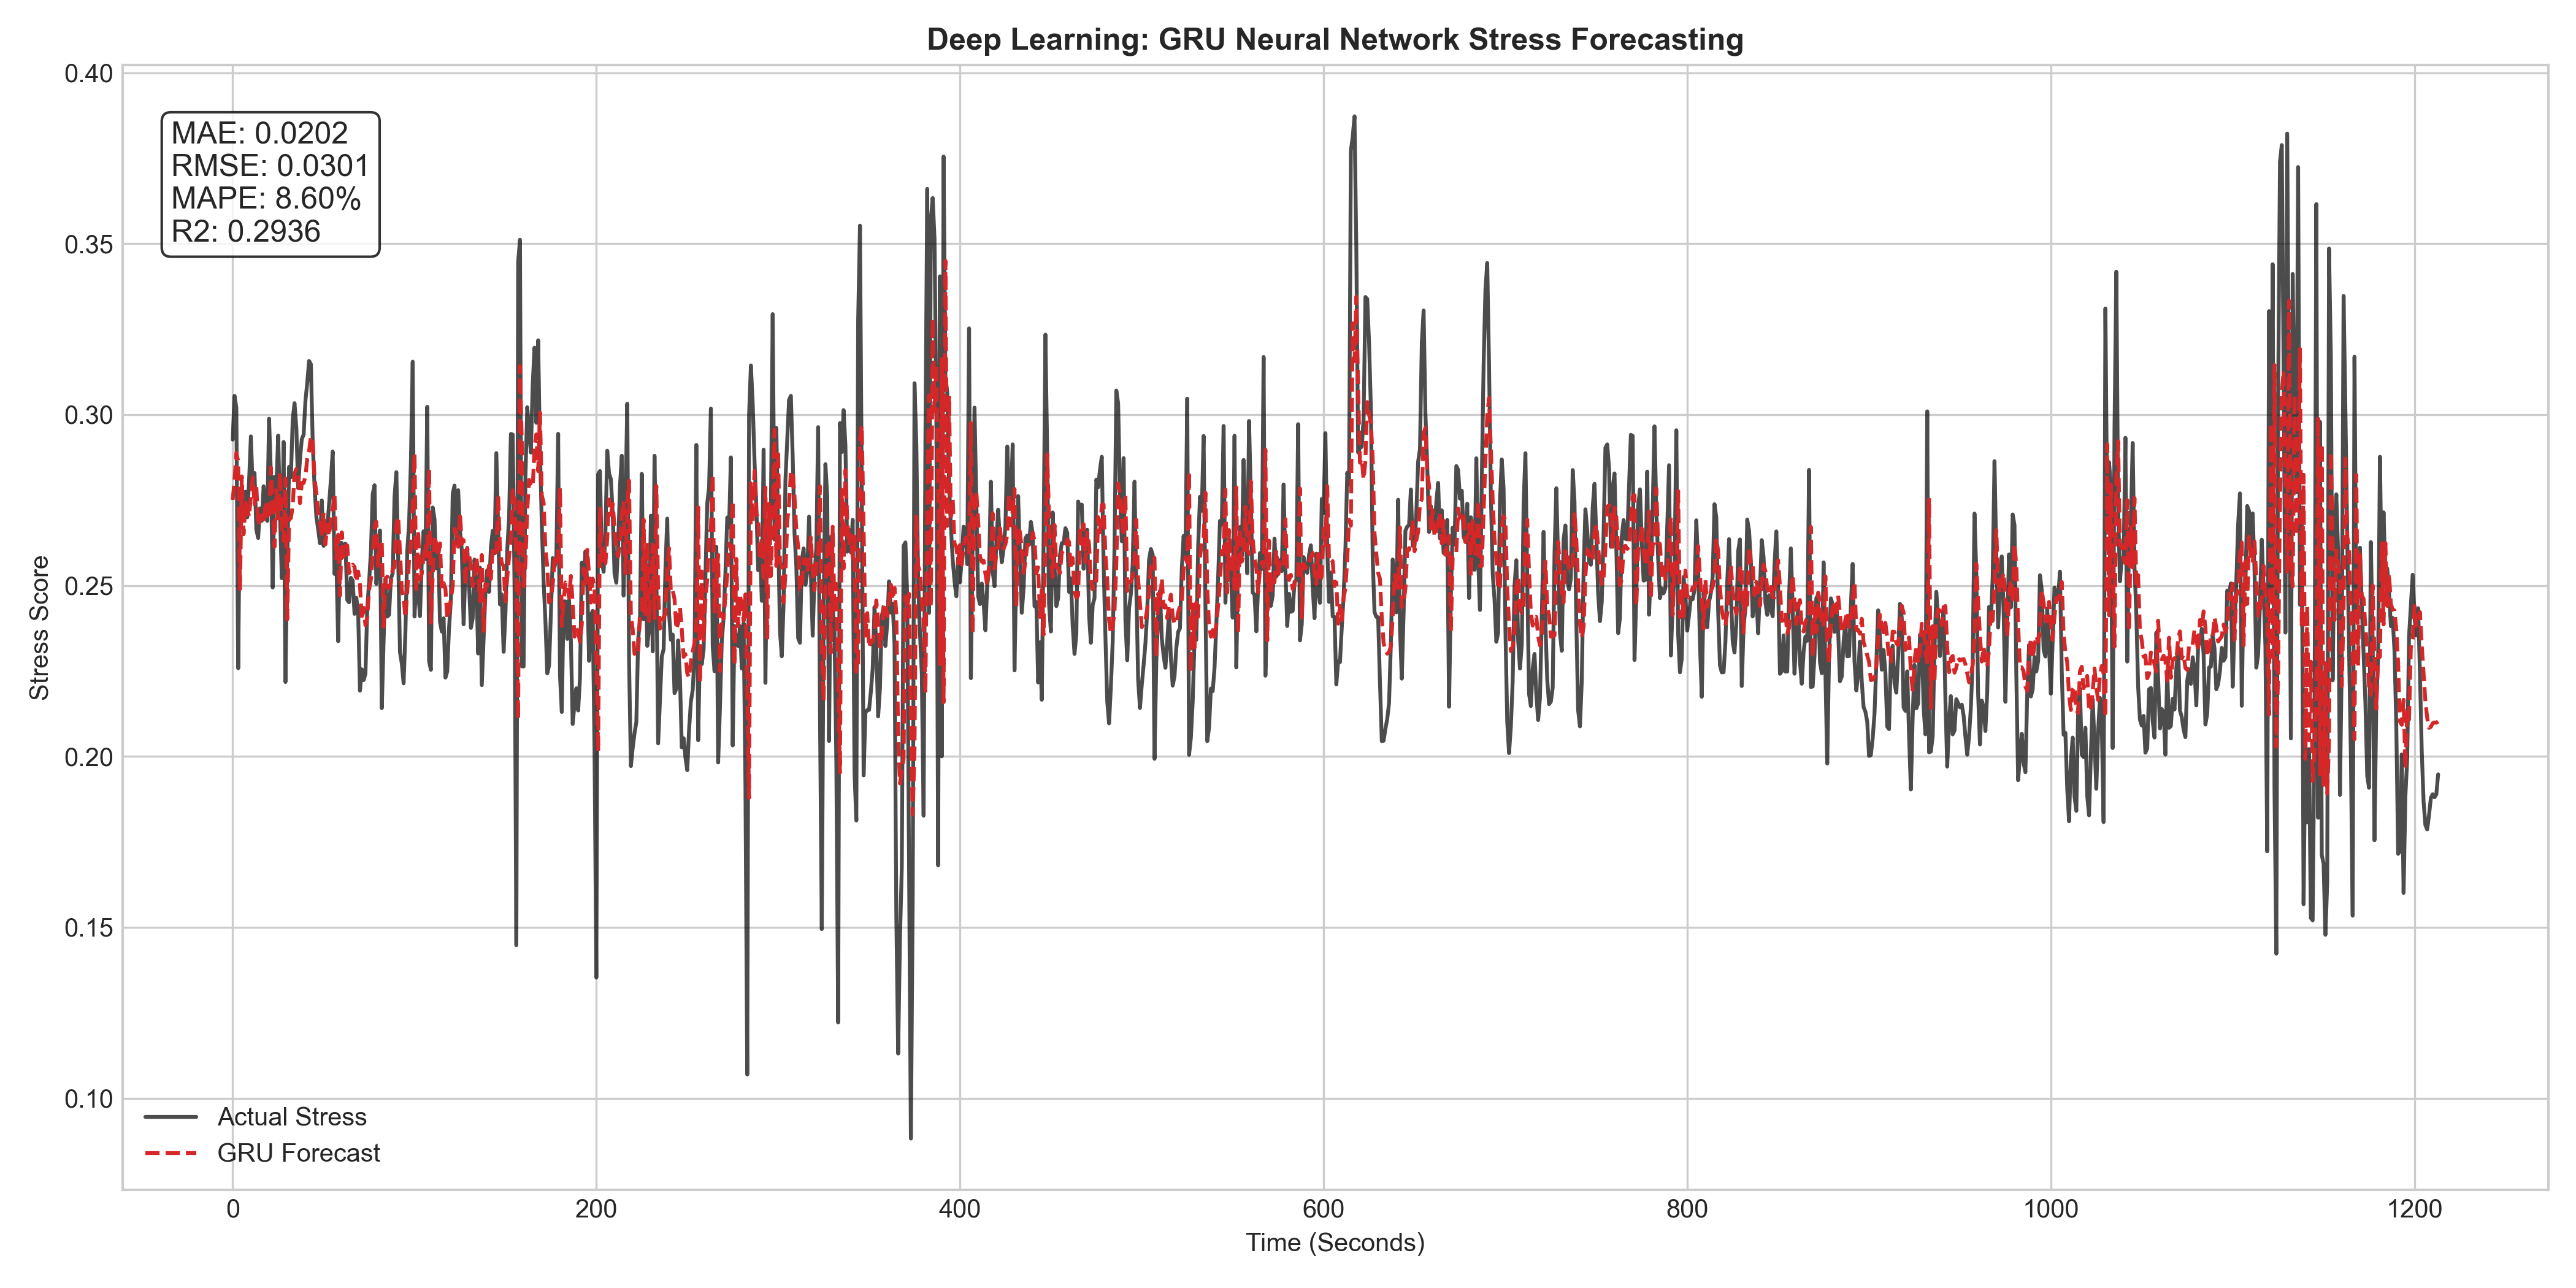
\includegraphics[width=1.0\textwidth]{Forecasting_Graphs/12_GRU_Forecast.png}
    \end{column}
    \begin{column}{0.3\textwidth}
        \textbf{Theory:}\\
        A streamlined LSTM with fewer gates. Highly efficient for high-frequency signal processing.\\[0.4cm]
        \slidemetrics{GRU}{0.0202}{0.0301}{8.60}{0.2936}
    \end{column}
\end{columns}
\end{frame}

\begin{frame}{Model 13: Risk Boundaries (Quantile Regression)}
\begin{columns}
    \begin{column}{0.65\textwidth}
        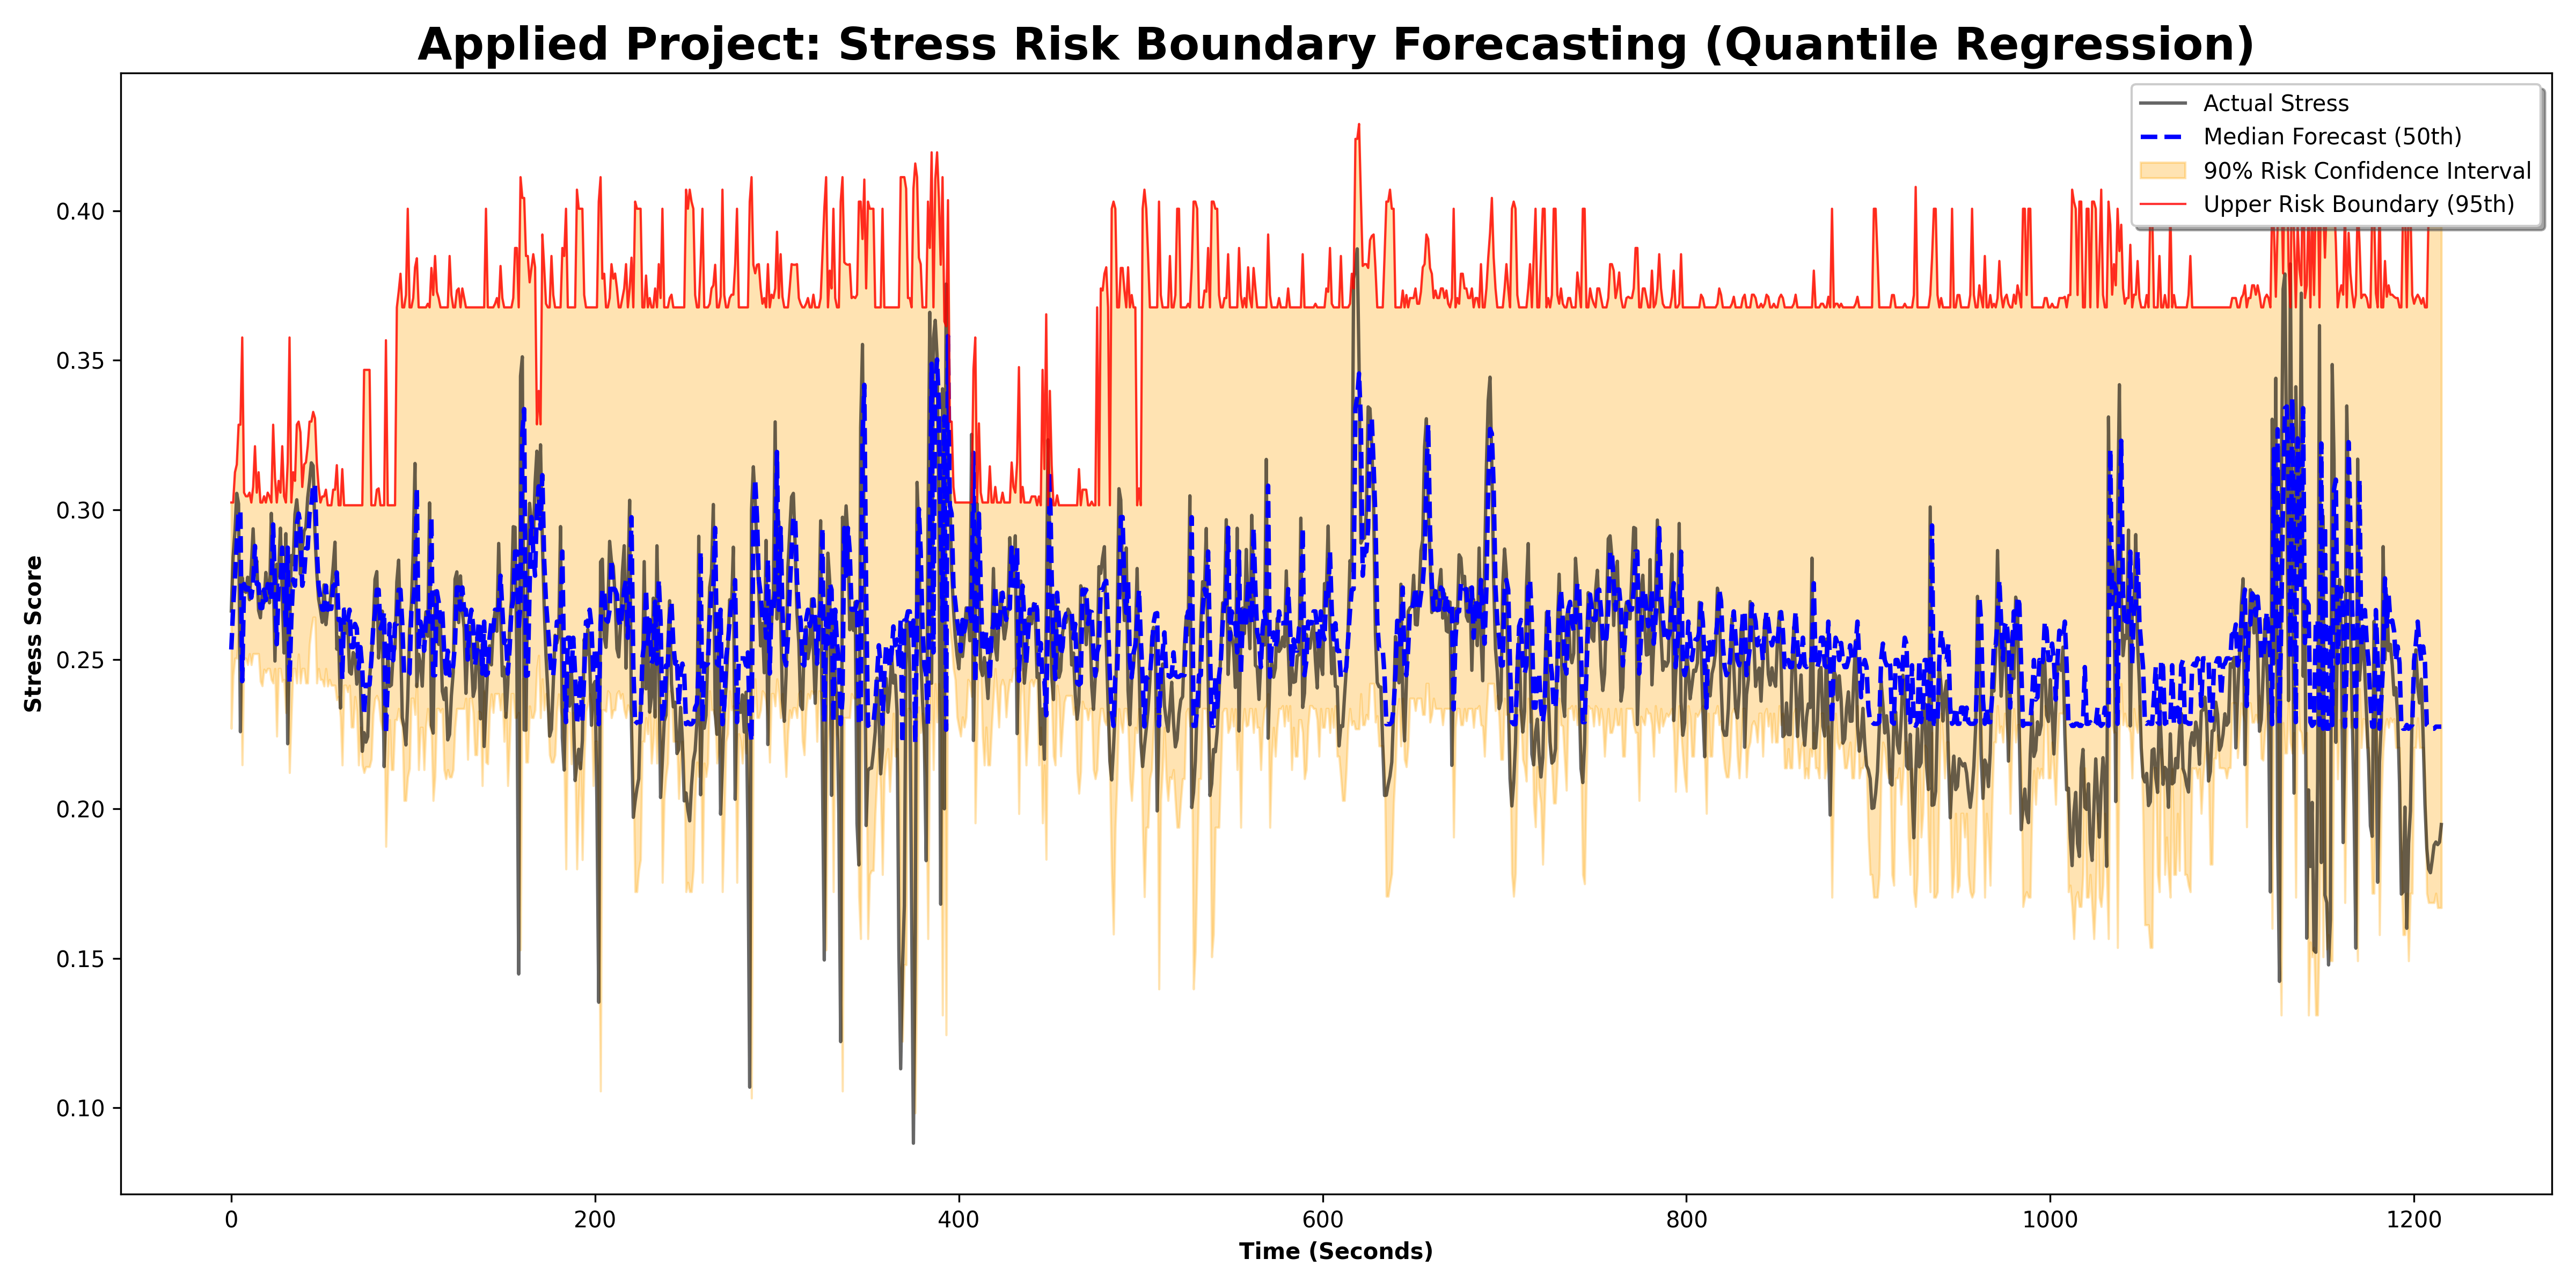
\includegraphics[width=1.0\textwidth]{Forecasting_Graphs/13_Quantile_Risk_Boundaries.png}
    \end{column}
    \begin{column}{0.3\textwidth}
        \textbf{Theory:}\\
        Minimizes \textbf{Pinball Loss} to forecast the 95th Percentile. Provides a crucial safety margin.\\[0.4cm]
        \slidemetrics{Quantile}{0.0241}{N/A}{N/A}{N/A}
    \end{column}
\end{columns}
\end{frame}

% ==========================================
% ANALYTICAL DEPTH
% ==========================================

\begin{frame}{Analytical Depth: Feature Ablation Study}
\textbf{Question:} Does adding wearable sensors (HR/EDA) actually improve predictions over just looking at past stress?
\begin{columns}
    \begin{column}{0.5\textwidth}
        \centering
        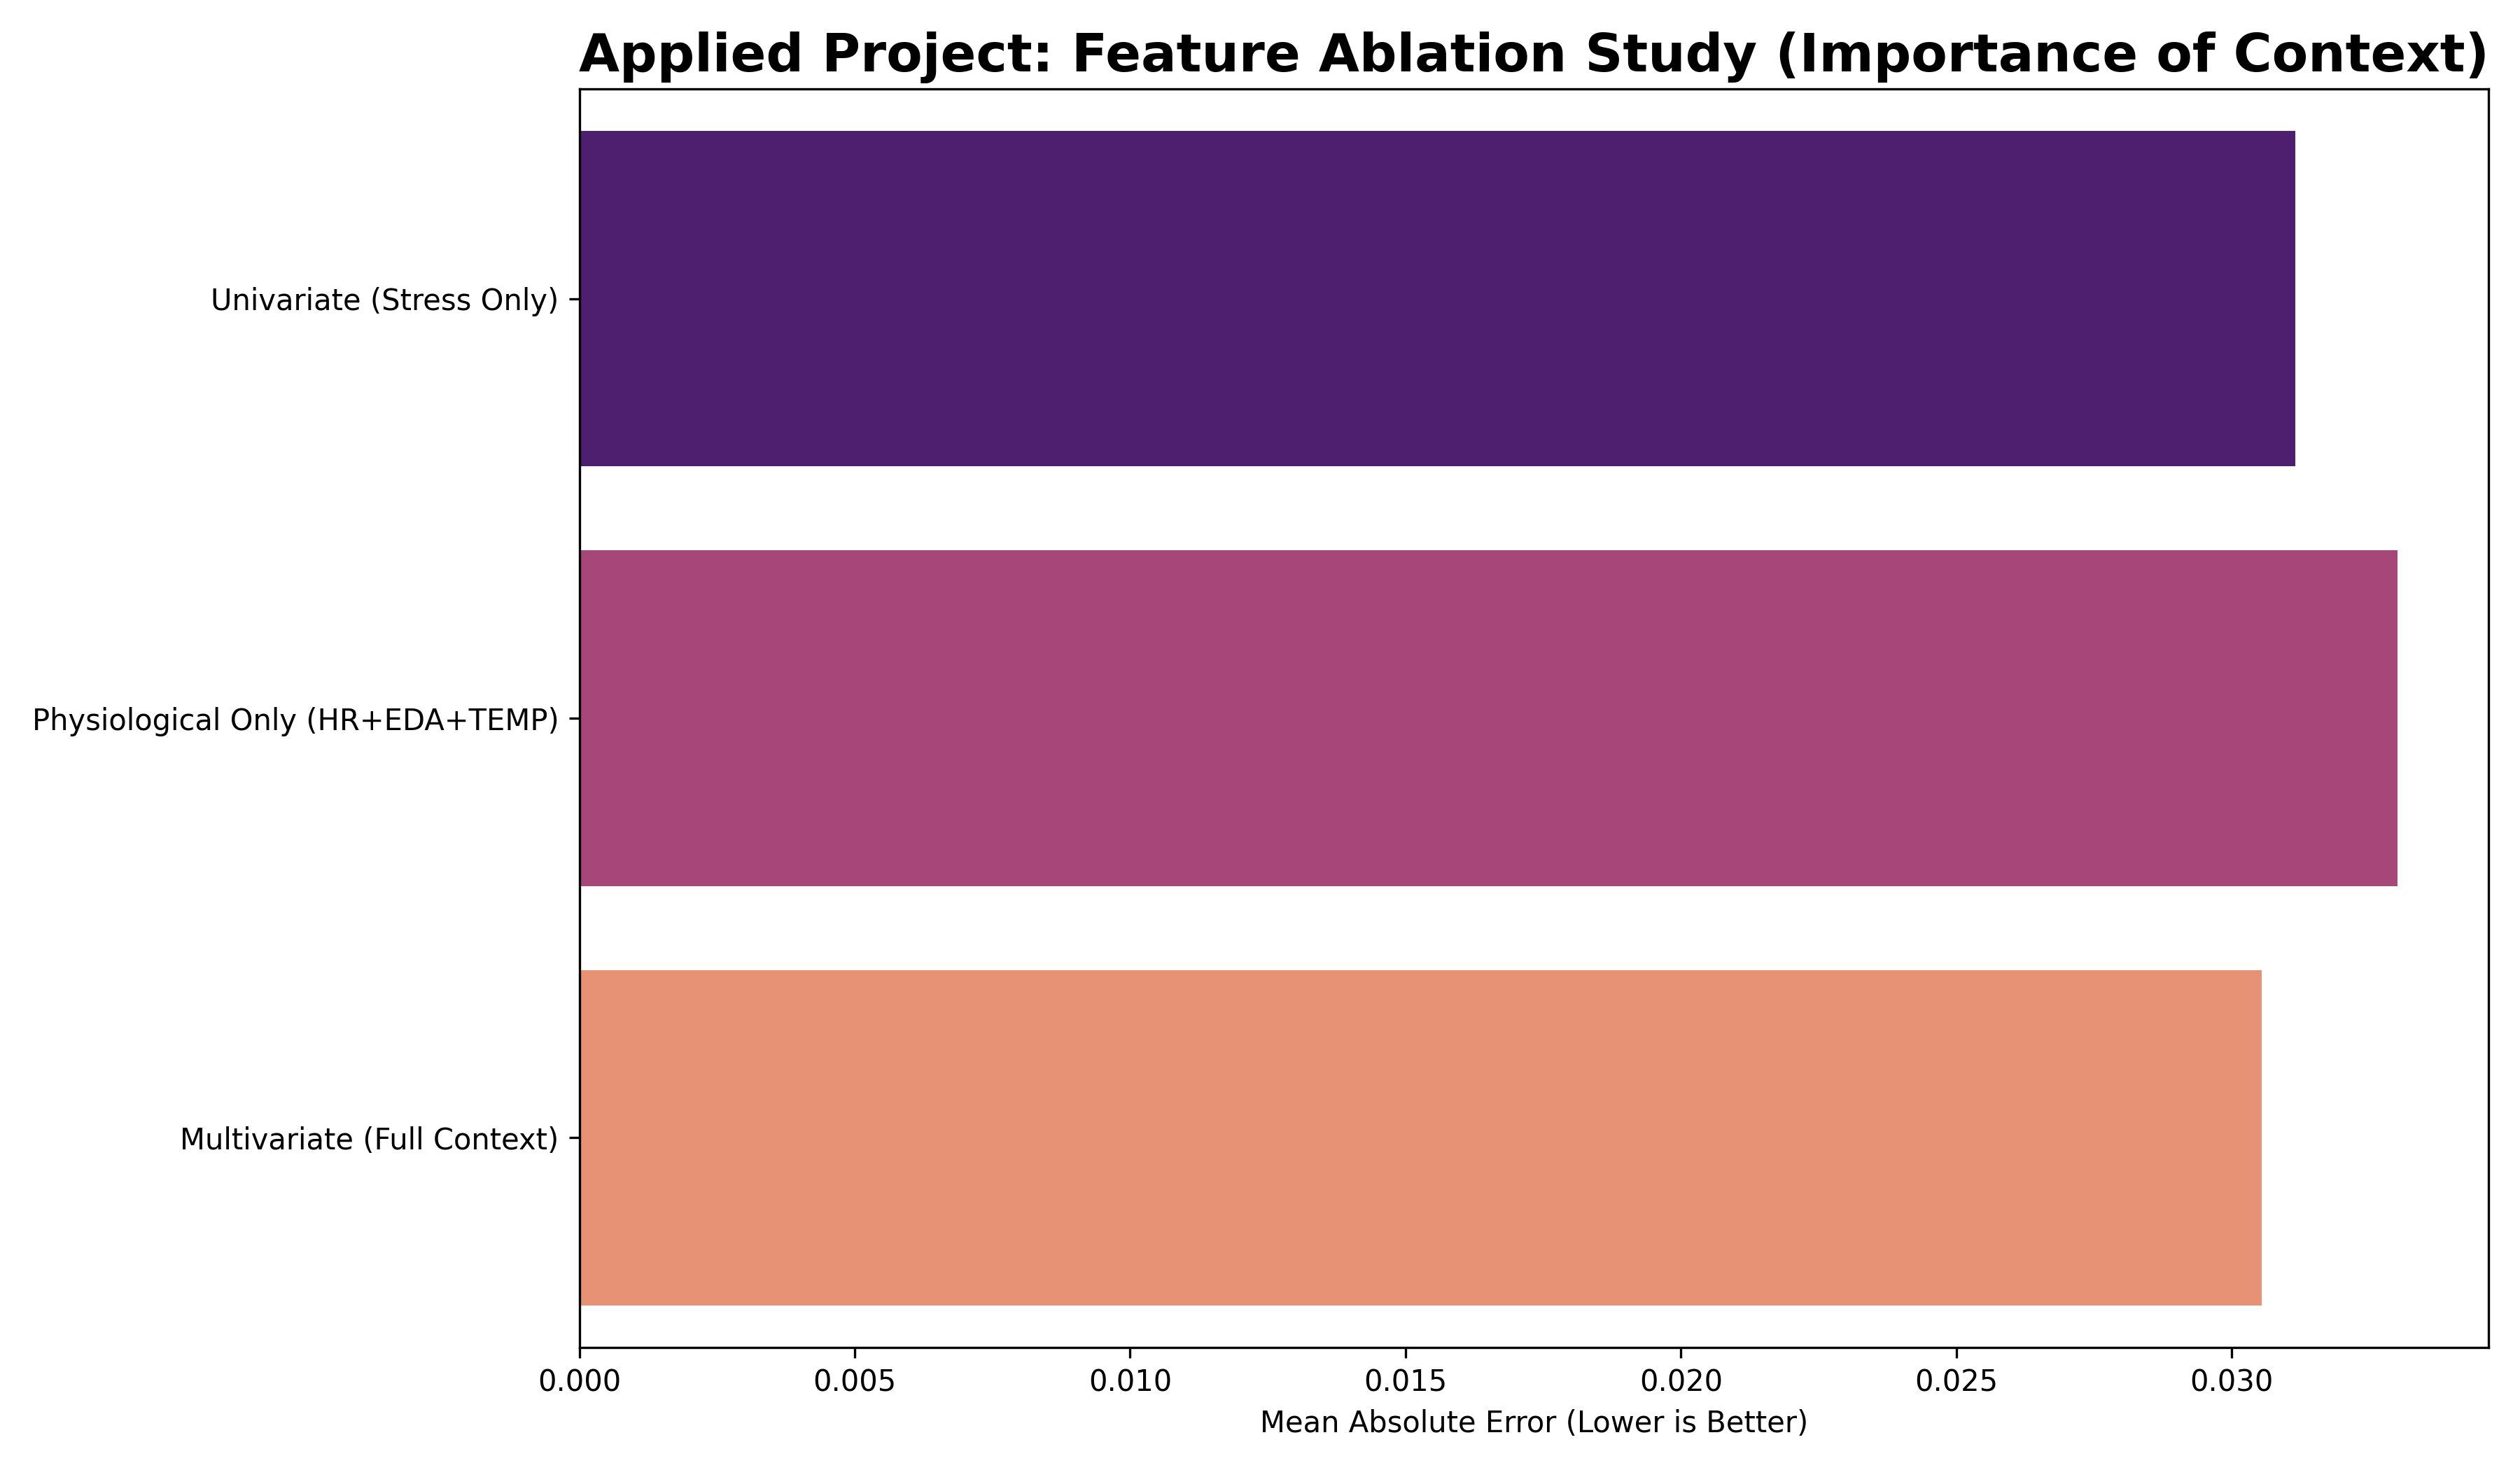
\includegraphics[width=1.0\textwidth]{EDA_Graphs/14_Feature_Ablation_Study.png}
    \end{column}
    \begin{column}{0.45\textwidth}
        \textbf{Findings:}\\[0.2cm]
        \begin{itemize}
            \item \textbf{Univariate:} MAE 0.0311
            \item \textbf{Sensors Only:} MAE 0.0330
            \item \textbf{\color{Emerald}Full Context:} MAE 0.0305
        \end{itemize}
        \vspace{0.2cm}
        Combining both history and physiological data provides the ultimate predictive edge.
    \end{column}
\end{columns}
\end{frame}

\begin{frame}{Analytical Depth: Forecast Horizon Decay}
\textbf{Question:} How far into the future can we predict before the error becomes unacceptable?
\begin{columns}
    \begin{column}{0.5\textwidth}
        \centering
        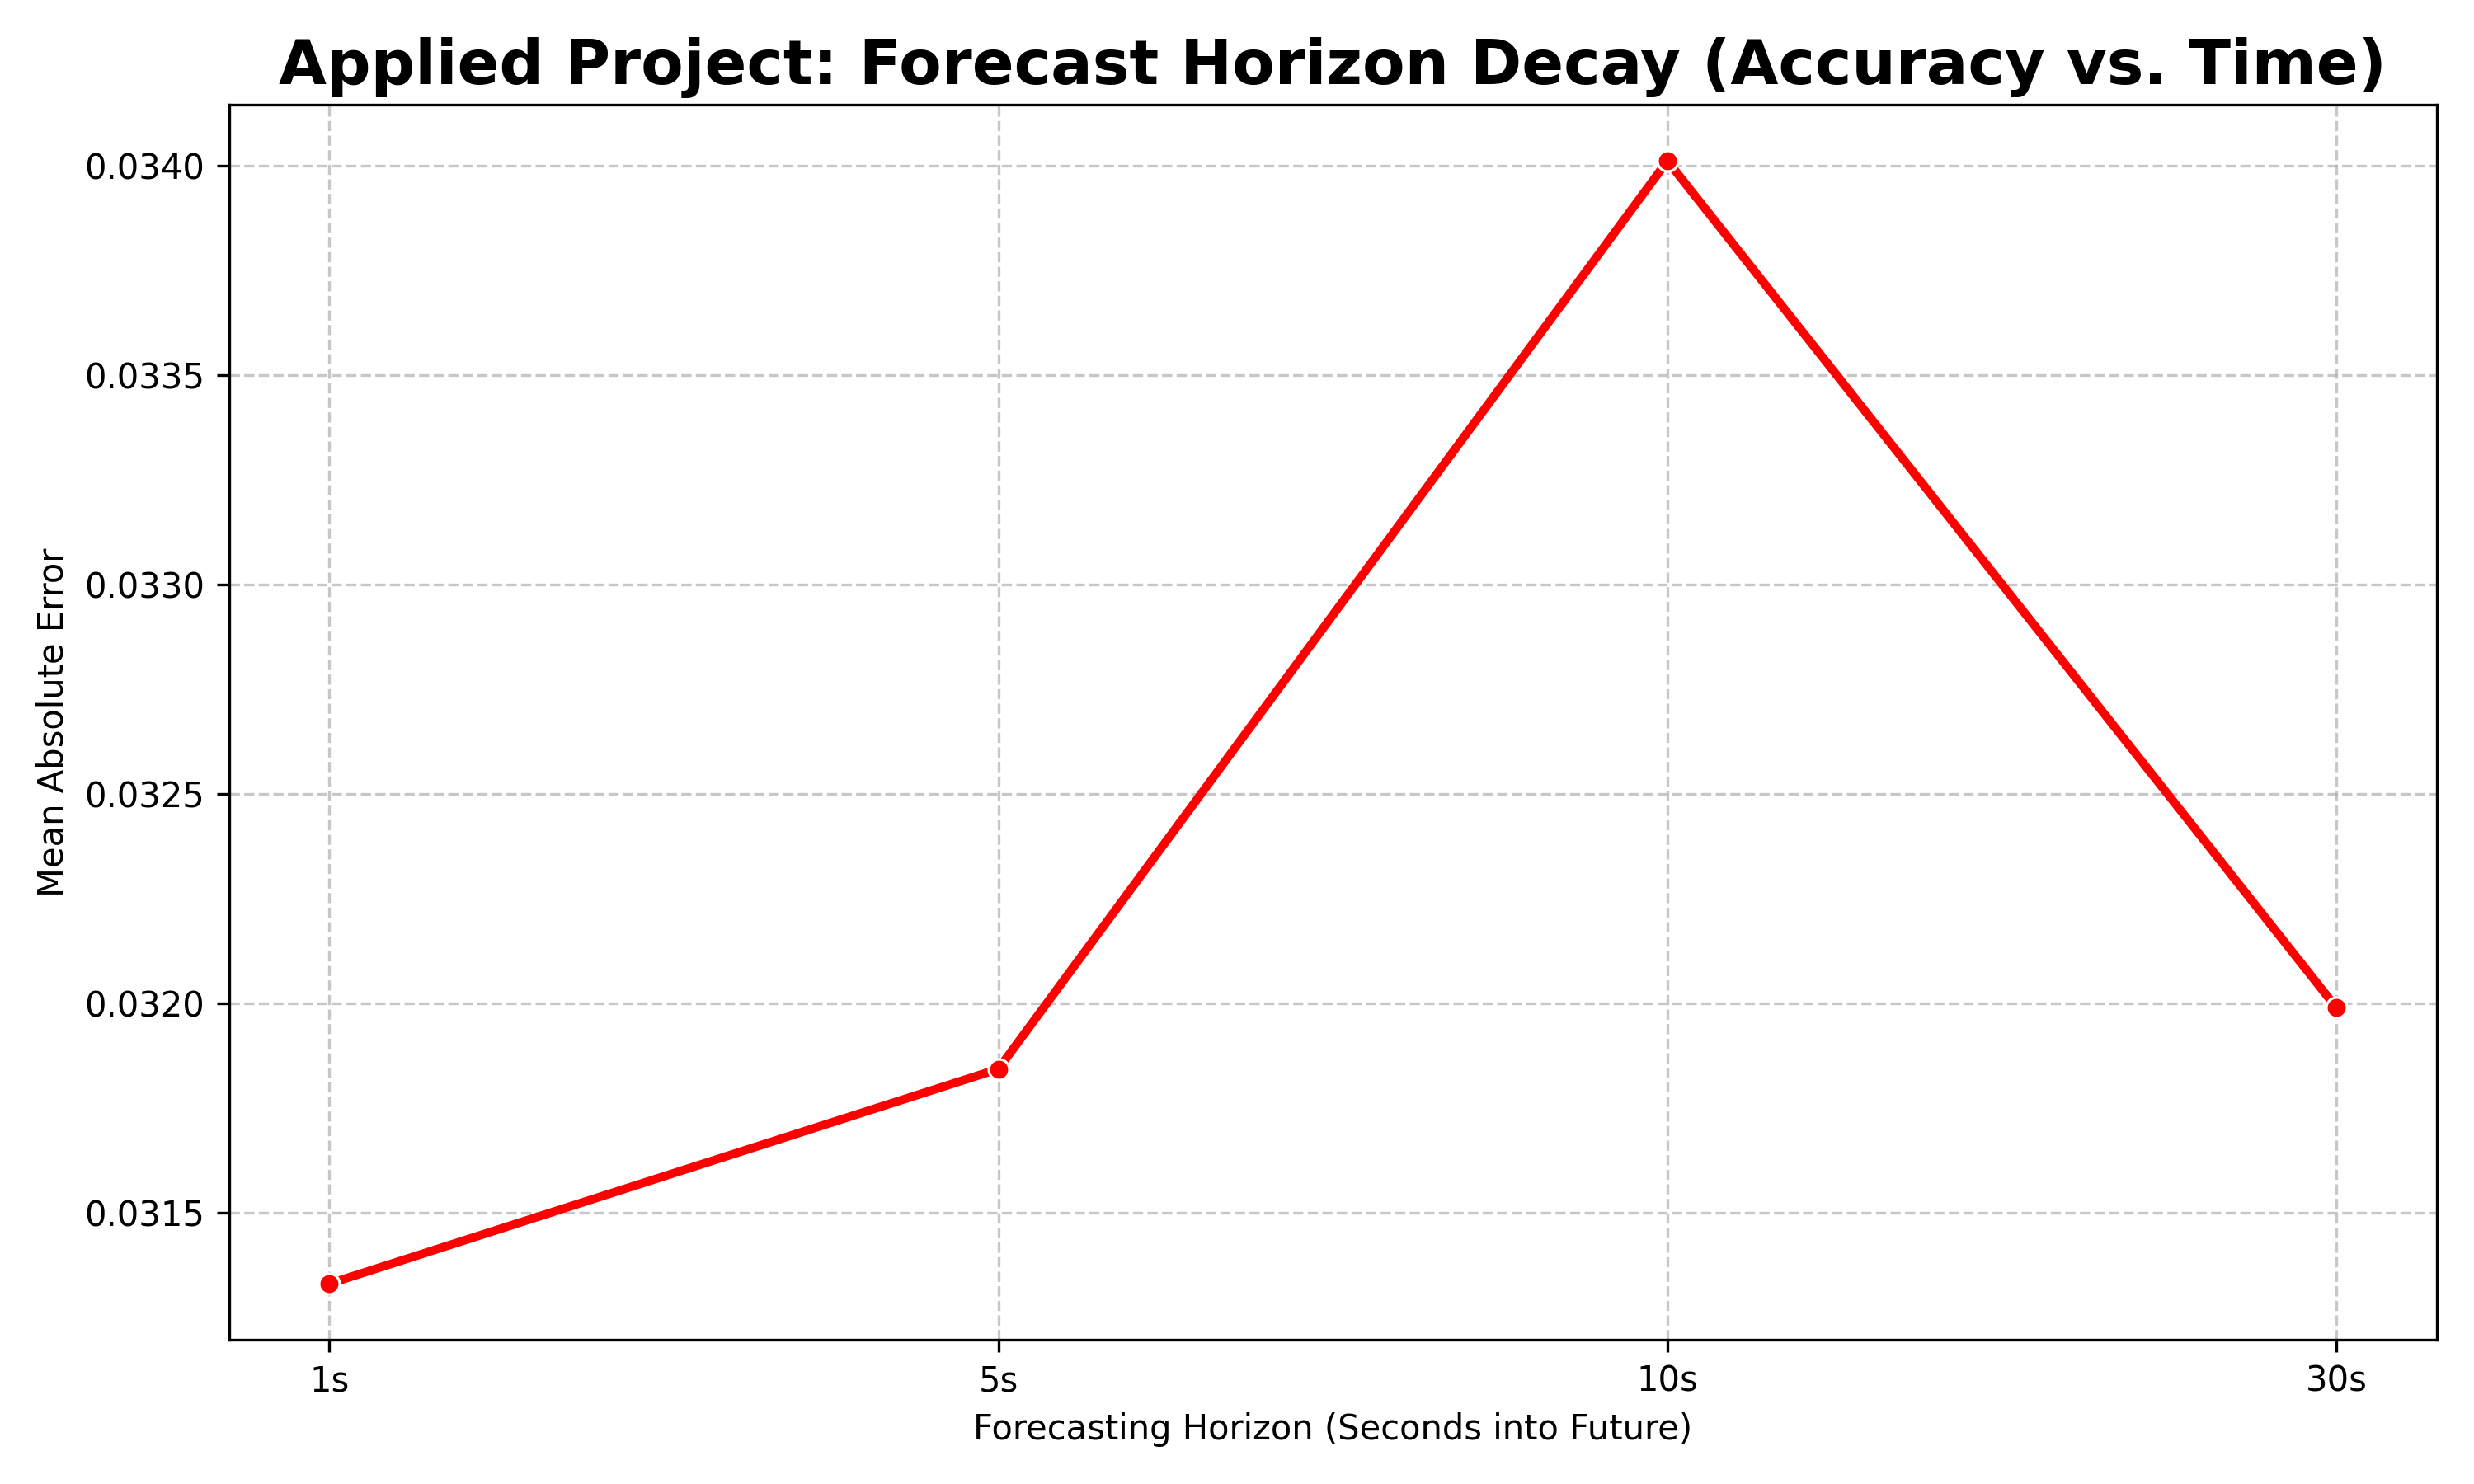
\includegraphics[width=1.0\textwidth]{EDA_Graphs/15_Horizon_Decay_Analysis.png}
    \end{column}
    \begin{column}{0.45\textwidth}
        \textbf{Findings:}\\[0.2cm]
        \begin{itemize}
            \item Performance remains remarkably stable up to \textbf{30 seconds} ahead.
            \item \textbf{Reason:} Physiological inertia. Once skin conductance begins to rise, the trajectory is highly deterministic.
        \end{itemize}
    \end{column}
\end{columns}
\end{frame}

\begin{frame}{Analytical Depth: Residual Diagnostics}
\textbf{Question:} Are the errors of our best models random (Gaussian), or are we systematically missing something?
\begin{columns}
    \begin{column}{0.6\textwidth}
        \centering
        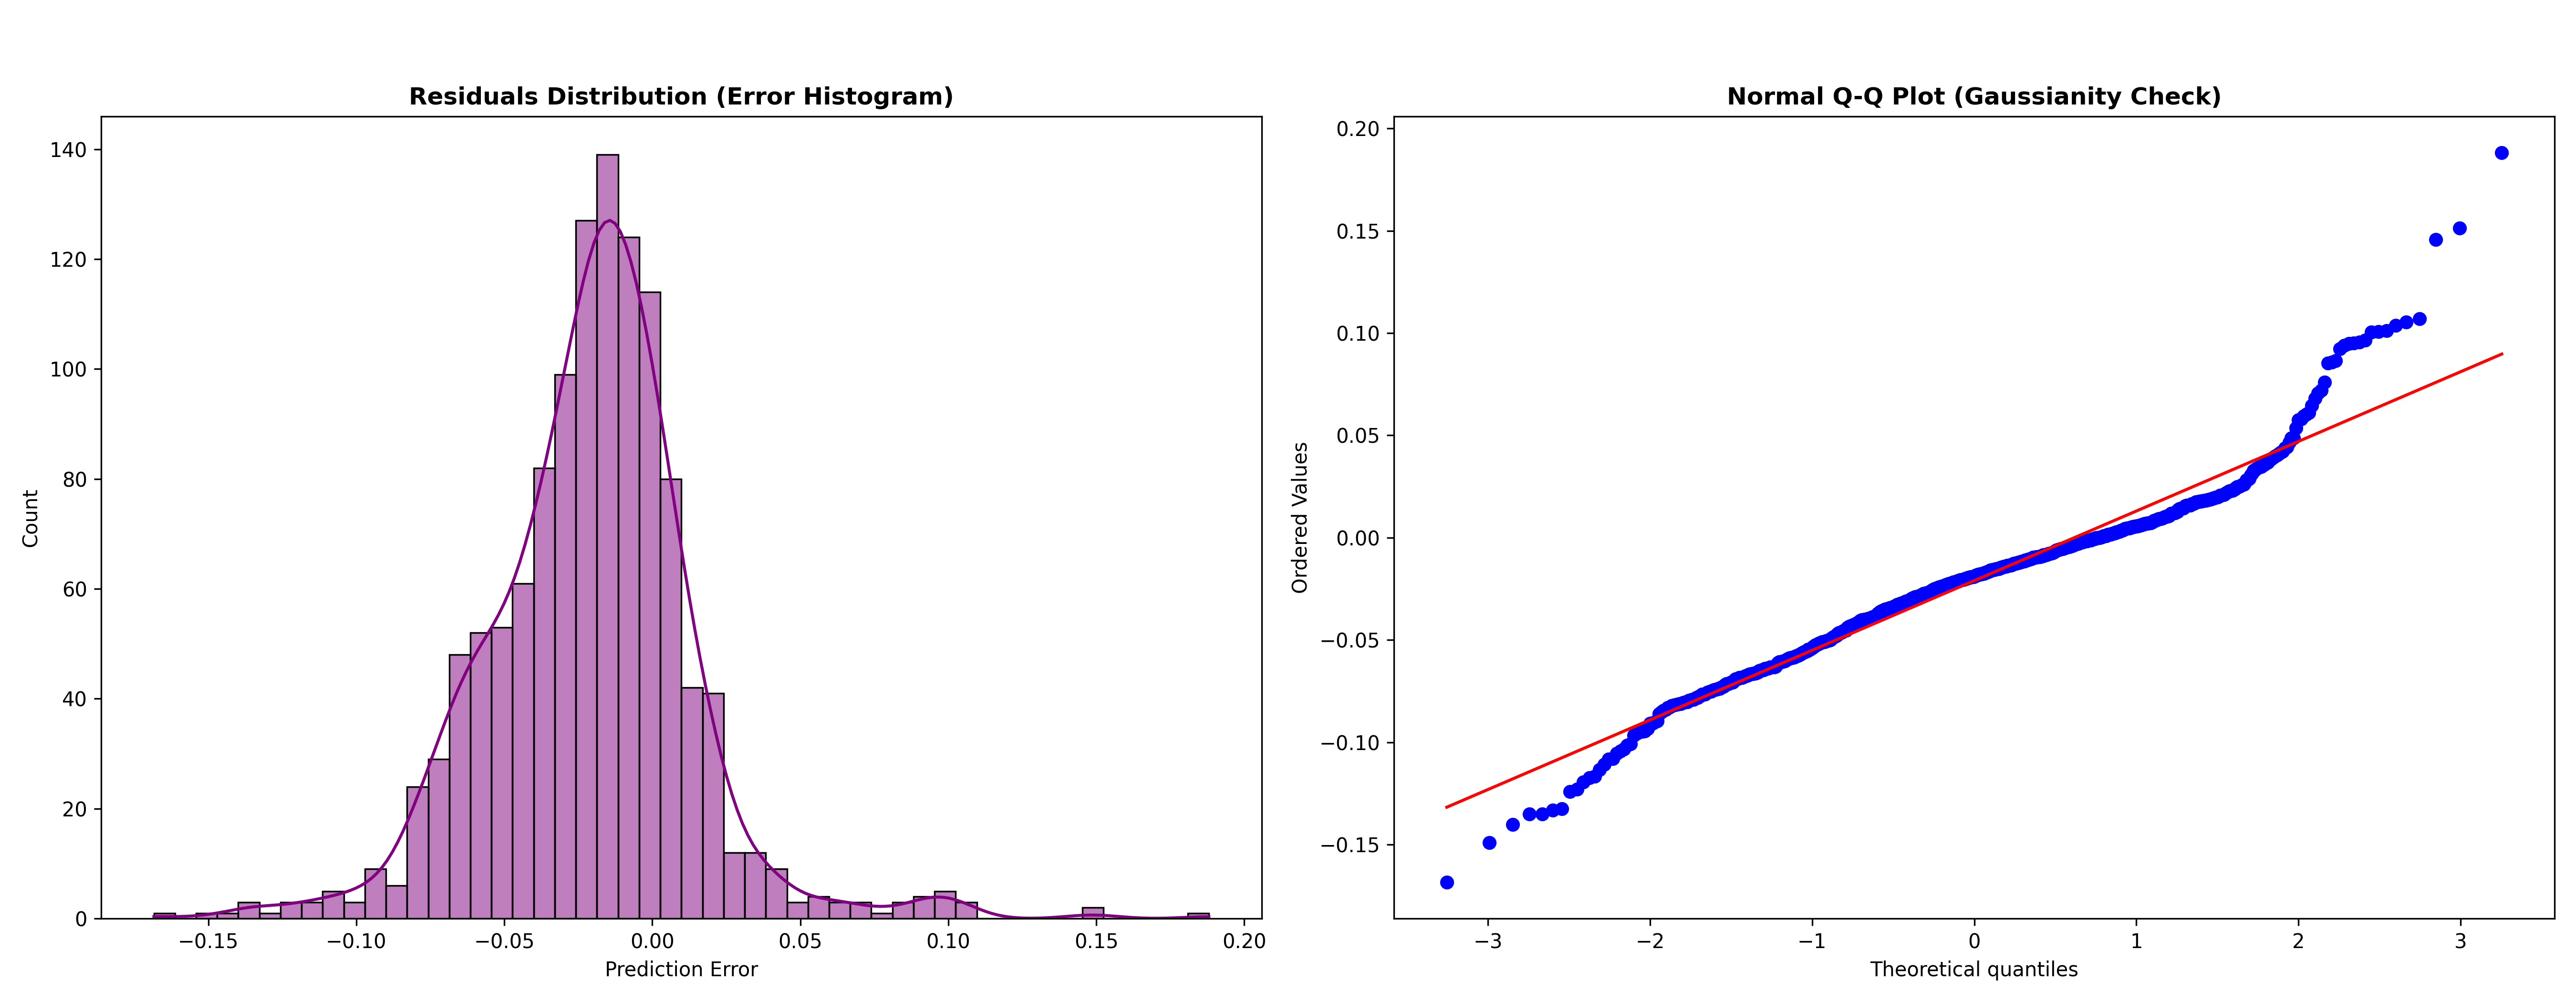
\includegraphics[width=1.0\textwidth]{EDA_Graphs/16_Residual_Analysis.png}
    \end{column}
    \begin{column}{0.35\textwidth}
        \textbf{Findings:}\\[0.2cm]
        The Q-Q plot confirms normal distribution near the mean, but shows "heavy tails". Models occasionally fail to capture abrupt, non-linear stress spikes.
    \end{column}
\end{columns}
\end{frame}

\begin{frame}{Analytical Depth: Cross-Subject Generalization}
\textbf{Question:} Can a model trained on Subject S2 be deployed blindly on Subject S3?
\begin{columns}
    \begin{column}{0.5\textwidth}
        \centering
        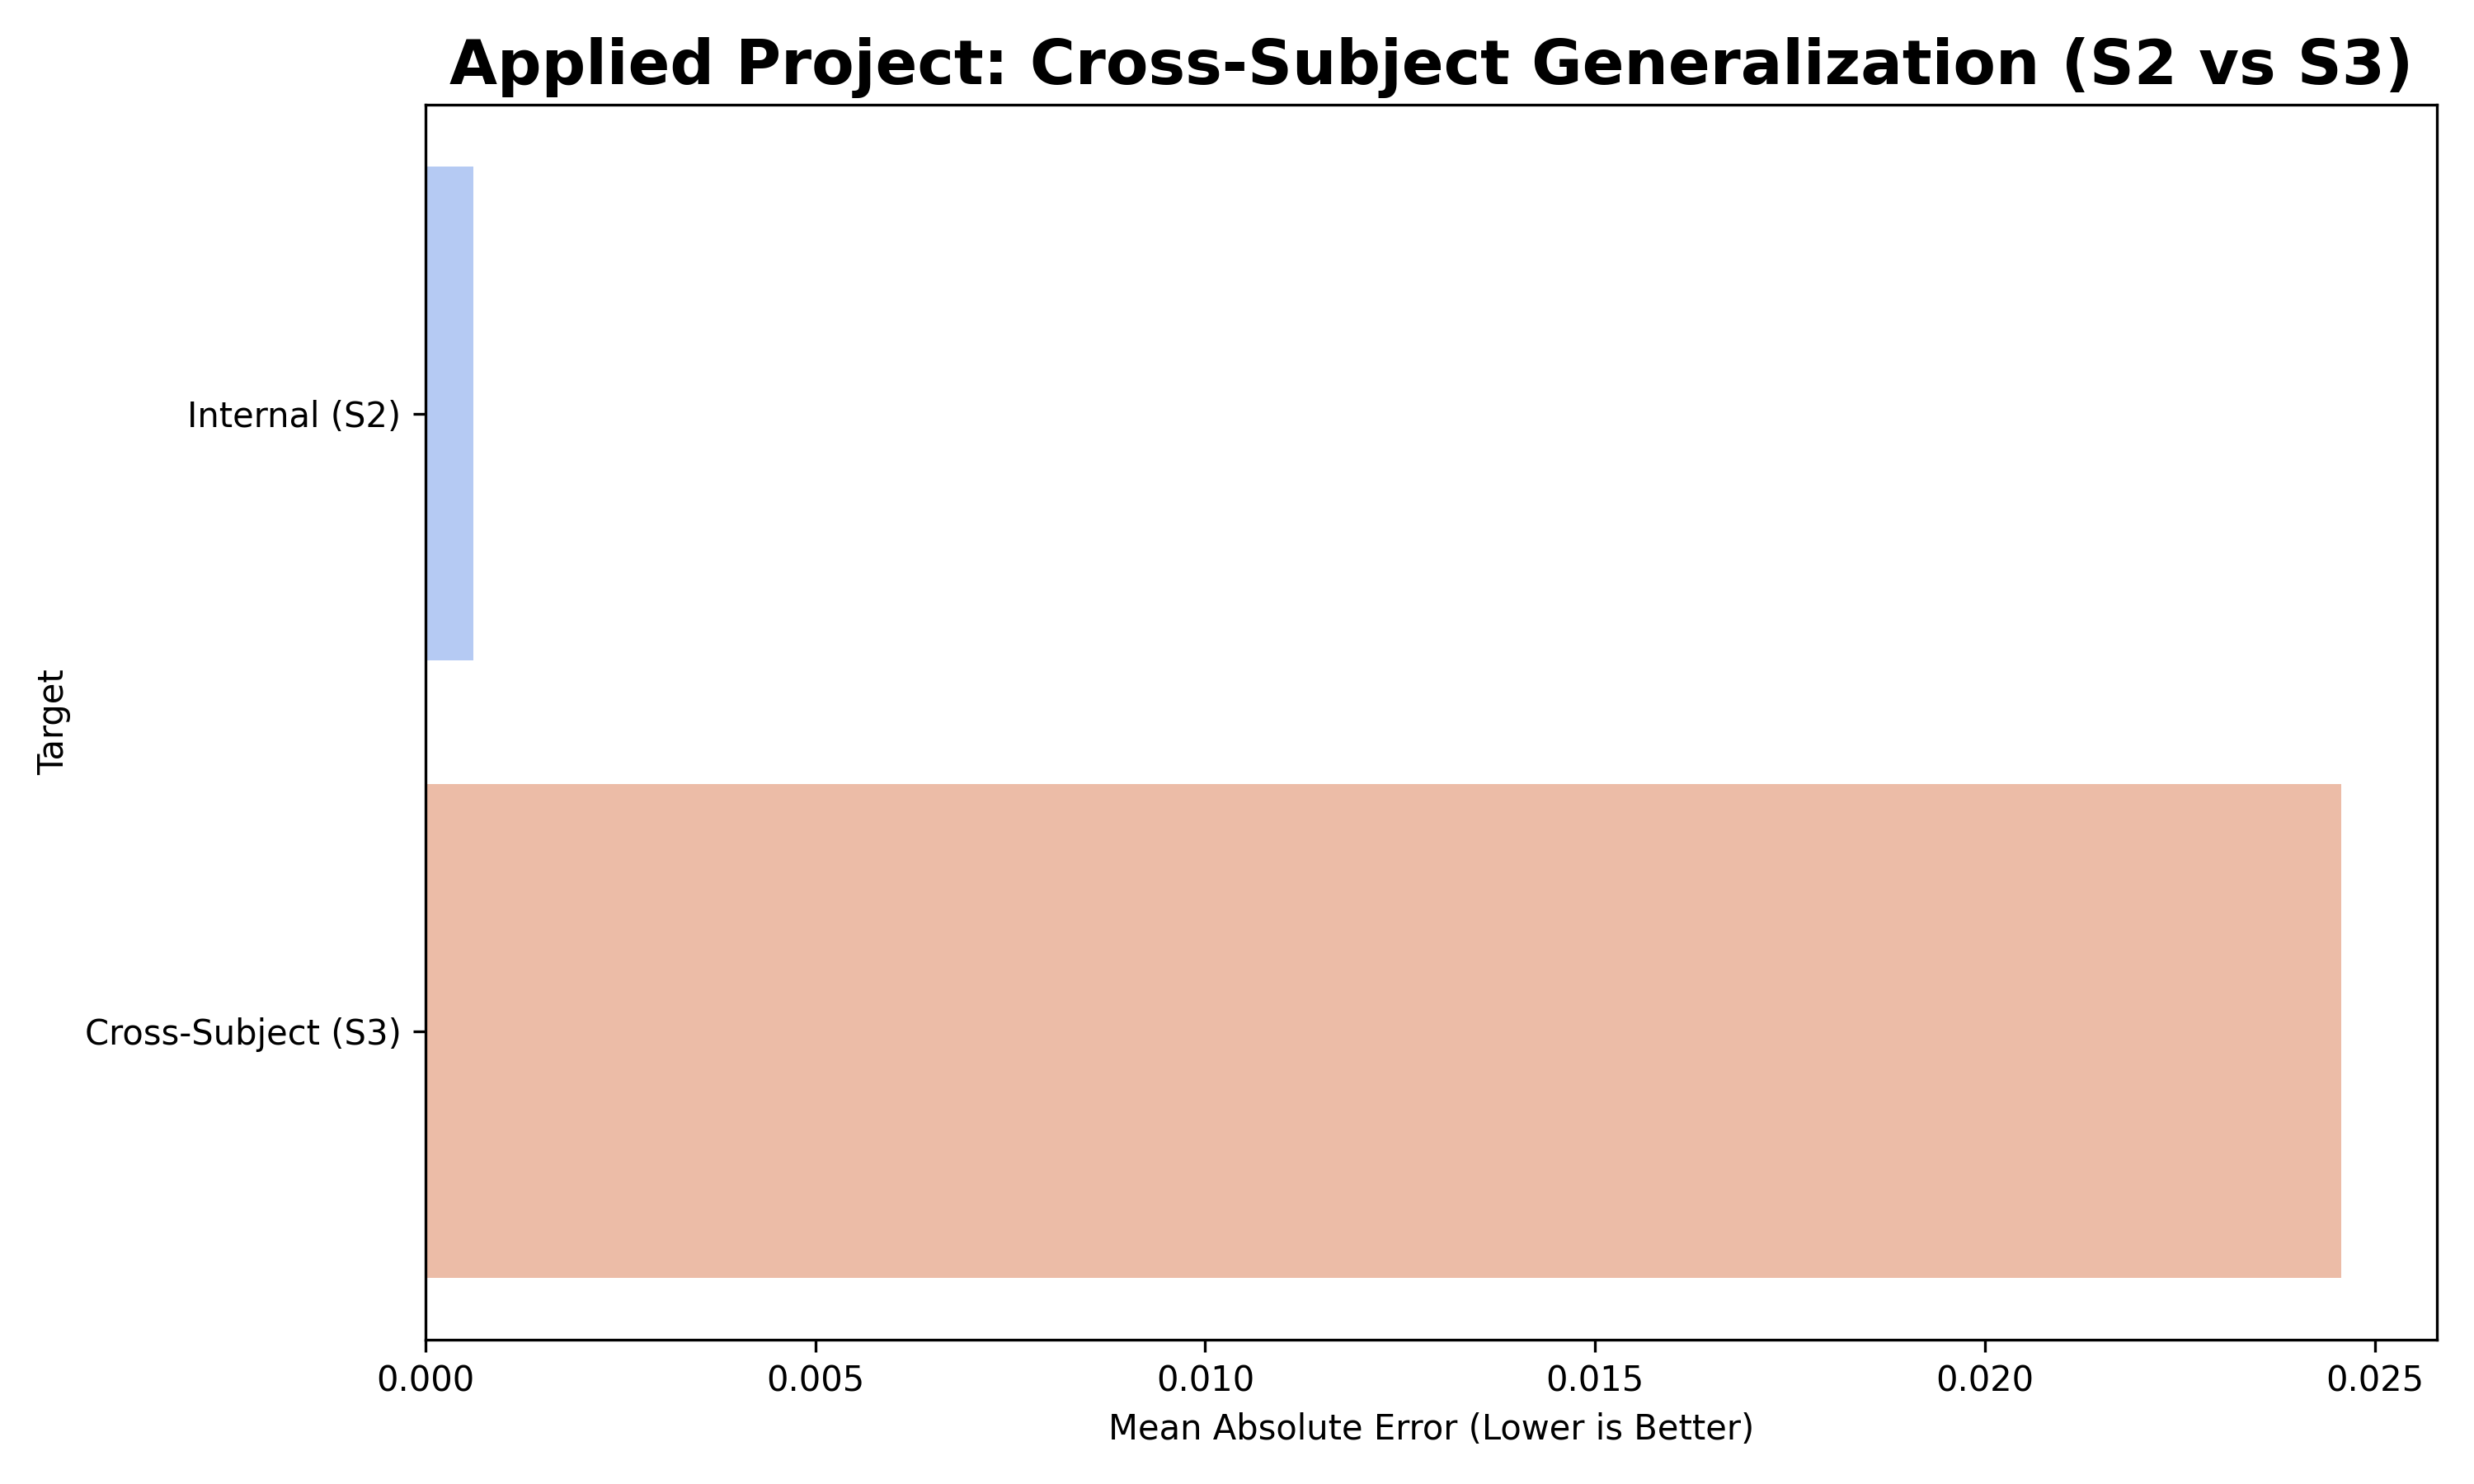
\includegraphics[width=1.0\textwidth]{EDA_Graphs/17_Generalization_Test.png}
    \end{column}
    \begin{column}{0.45\textwidth}
        \textbf{Findings:}\\[0.2cm]
        \begin{itemize}
            \item \textbf{Internal MAE:} 0.0006
            \item \textbf{S3 Transfer MAE:} 0.0246
        \end{itemize}
        \vspace{0.2cm}
        Stress signatures are highly personalized. Real-world deployment requires user-specific calibration (Transfer Learning).
    \end{column}
\end{columns}
\end{frame}

% ==========================================
% FINAL LEADERBOARD
% ==========================================
\begin{frame}{Final Leaderboard: Ranked by MAPE}
\begin{center}
\renewcommand{\arraystretch}{1.2}
\small
\begin{tabular}{clcccc}
    \toprule
    \rowcolor{Navy!10} \textbf{Rank} & \textbf{Model} & \textbf{MAPE} & \textbf{MAE} & \textbf{RMSE} & \textbf{R$^2$} \\
    \midrule
    \rowcolor{Emerald!20} \textbf{1} & \textbf{LSTM (Deep Learning)} & \textbf{8.40\%} & \textbf{0.0198} & \textbf{0.0298} & \textbf{0.3057} \\
    2 & ARMA (2,3) & 8.60\% & 0.0206 & 0.0316 & 0.2204 \\
    3 & GRU (Deep Learning) & 8.60\% & 0.0202 & 0.0301 & 0.2936 \\
    4 & AR (p=2) & 8.66\% & 0.0210 & 0.0342 & 0.0840 \\
    5 & Naive Baseline & 8.68\% & 0.0211 & 0.0345 & 0.0673 \\
    6 & MA (q=3) & 8.72\% & 0.0209 & 0.0335 & 0.1236 \\
    7 & SVR (Machine Learning) & 8.77\% & 0.0208 & 0.0314 & 0.2309 \\
    8 & SARIMA & 9.55\% & 0.0230 & 0.0348 & 0.0537 \\
    9 & SMA-10 & 9.62\% & 0.0229 & 0.0326 & 0.1716 \\
    10 & XGBoost & 10.06\% & 0.0230 & 0.0323 & 0.1840 \\
    \bottomrule
\end{tabular}
\end{center}
\end{frame}

% ==========================================
% DASHBOARD
% ==========================================
\begin{frame}{Performance Dashboard}
\centering
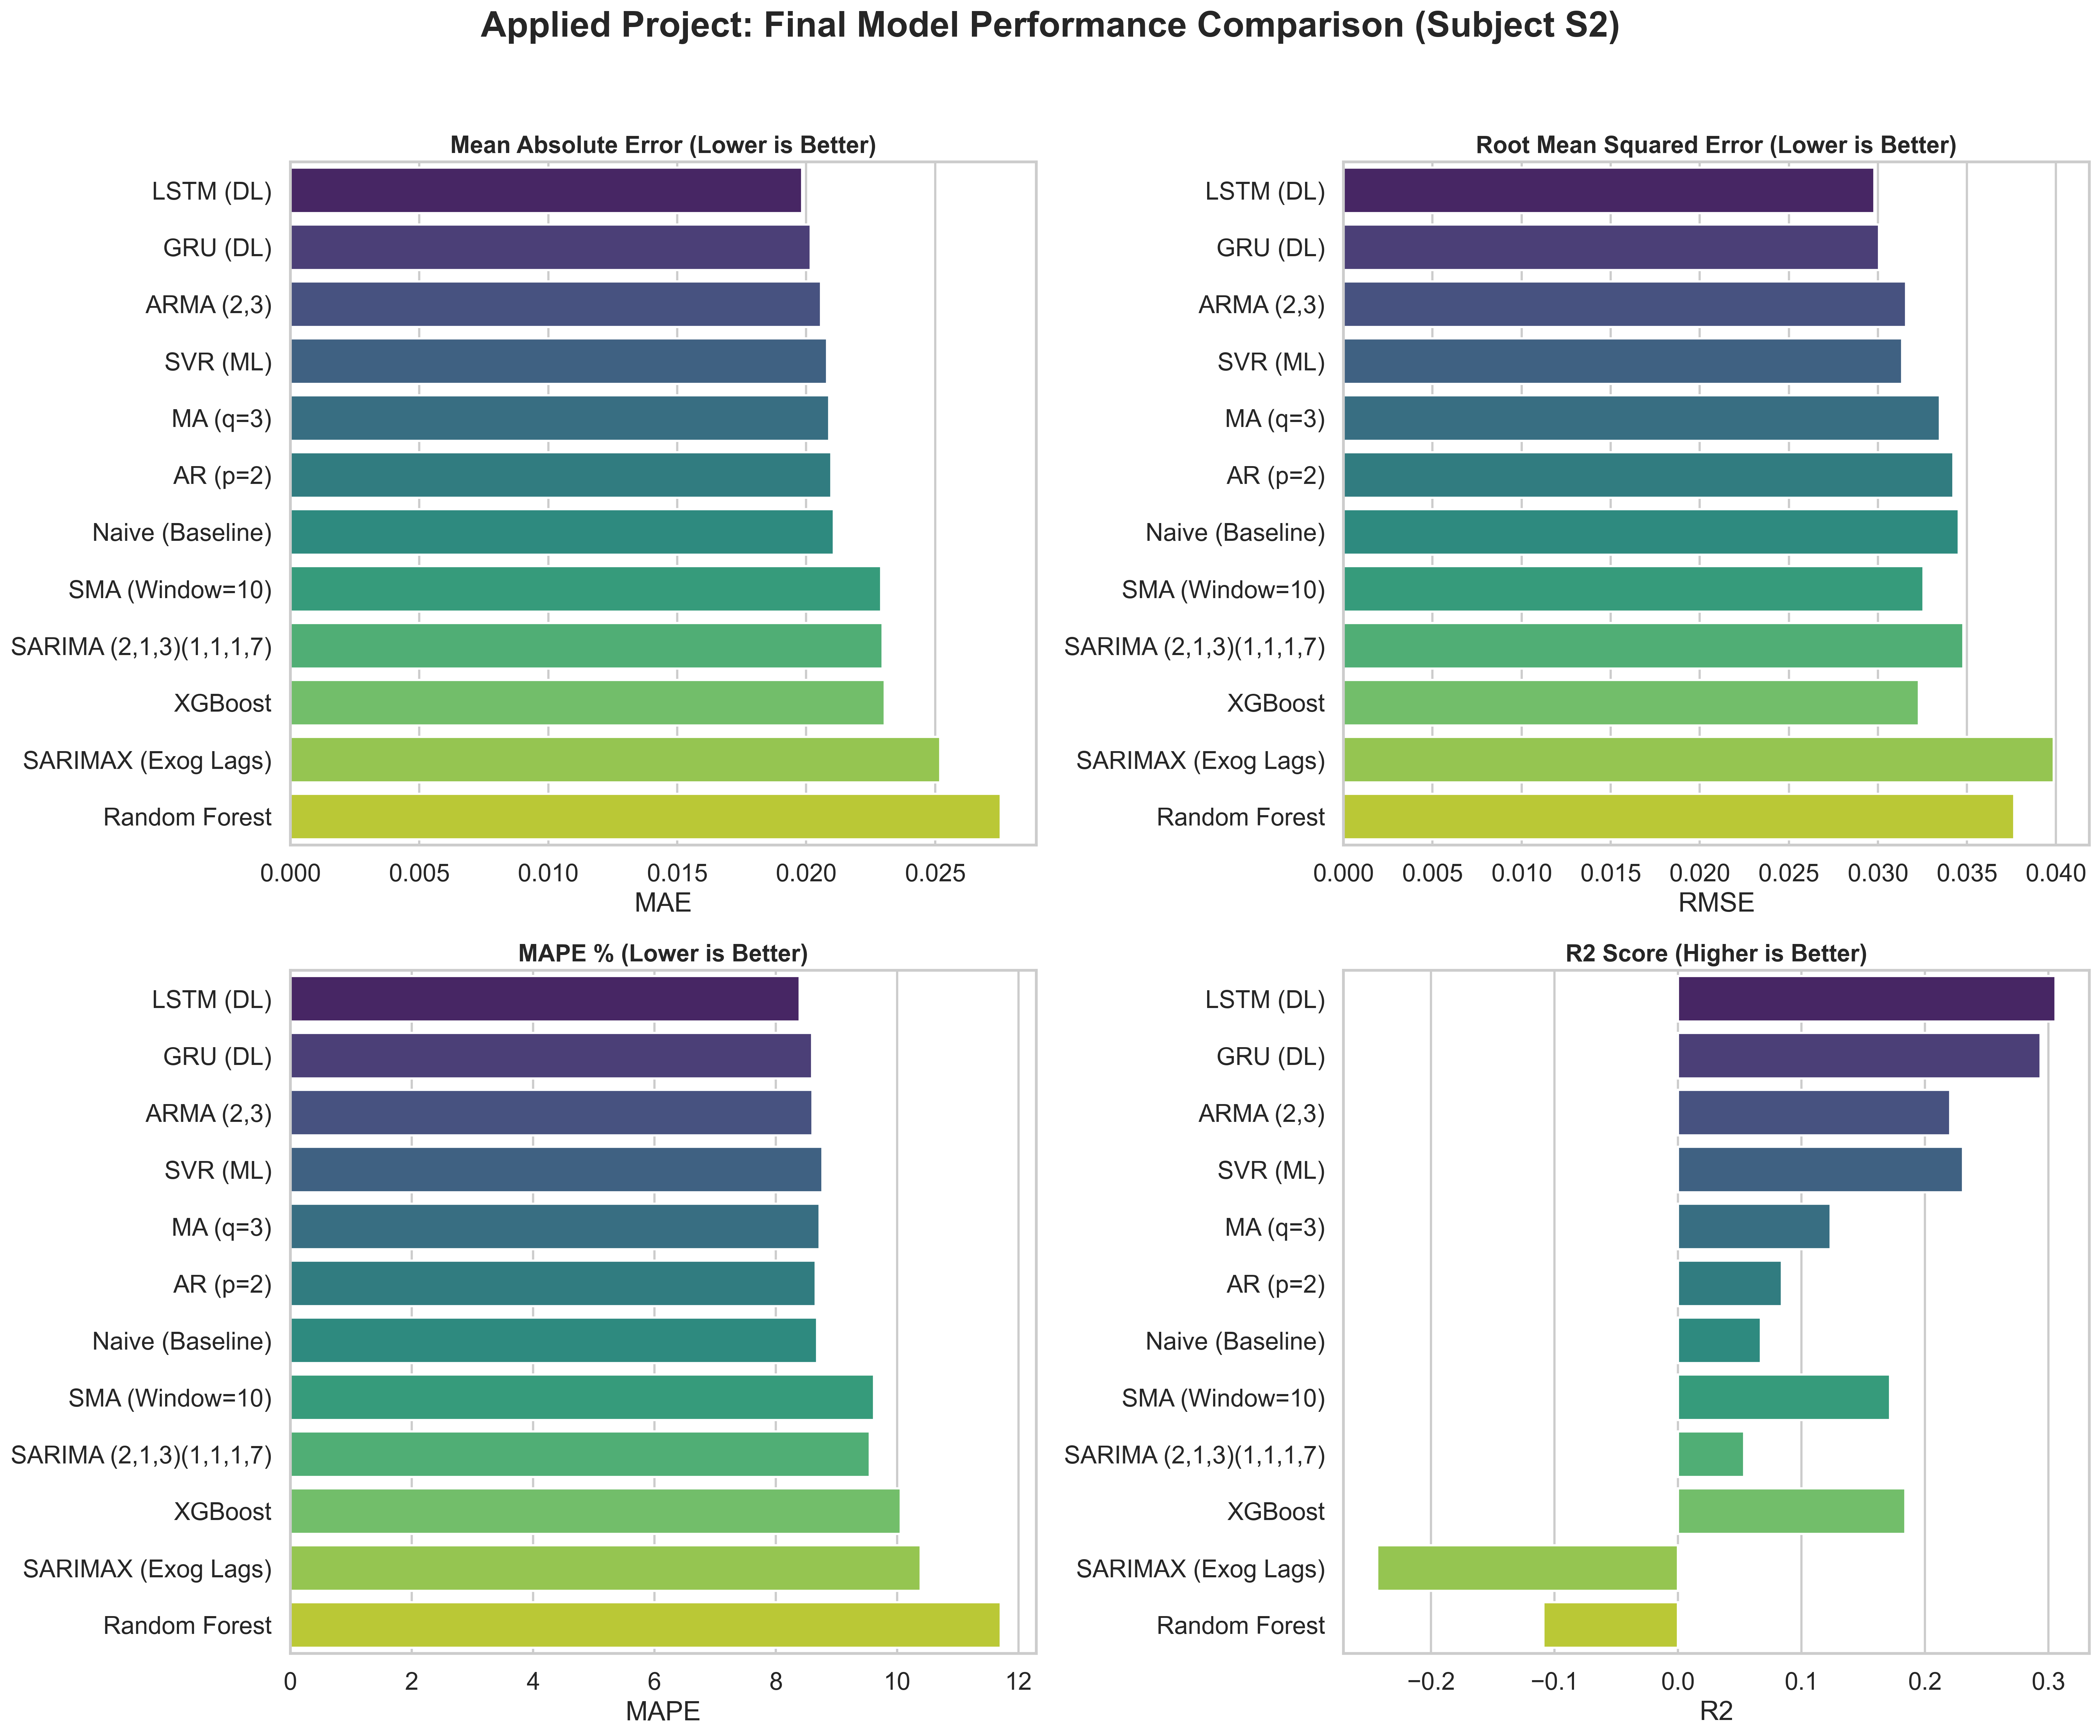
\includegraphics[width=0.9\textwidth]{Forecasting_Graphs/99_Final_Model_Comparison.png}
\end{frame}

% ==========================================
% CONCLUSION & Q&A
% ==========================================
\begin{frame}[plain]

\begin{tikzpicture}[remember picture, overlay]
    \fill[Navy] (current page.north west) rectangle (current page.south east);
    \fill[Emerald] (current page.south west) -- ($(current page.south west) + (3,0)$) -- ($(current page.north west) + (0, 3)$) -- cycle;

    \node[anchor=center, white] at (current page.center) {
        \begin{minipage}{\textwidth}
            \centering
            {\fontsize{40}{48}\selectfont \textbf{Thank You!}}\\[1cm]
            {\color{Emerald}\large \textbf{Questions \& Technical Discussion}}\\[1.5cm]
            {\color{LightGray!70}\small Applied Forecasting Methods}\\[0.2cm]
            {\color{LightGray!70}\scriptsize DHIRUBHAI AMBANI INSTITUTE (DA-IICT)}
        \end{minipage}
    };
\end{tikzpicture}
\end{frame}

\end{document}
